\begin{frame}
\begin{center}
\Huge Four \textcolor{mygreen}{methods} to compute the air pollution \textcolor{mypurple}{health damage}
\end{center}
\end{frame}
%------------------------------------------------


% Value of Statistical Life %------------------------------------------------%------------------------------------------------%------------------------------------------------
\begin{frame}{Value of Statistical Life (VSL)}
% It is the local trade-off rate between fatality risk and money. When
% the trade-off values are derived from choices in market contexts, the VSL serves
% as both a measure of the population’s willingness to pay for risk reduction and the
% marginal cost of enhancing safety. This equation contains an elasticity constant,
% which its choice derives uncertainty as well
$$VSL_{i,t} = VSL_{R10EUROPE,2005} \cdot \left(\frac{\tikzmark{GDPpc}GDPpc_{i,t}}{GDPpc_{R10EUROPE,2005}} \right) ^ \alpha\tikzmark{aa}, \; \; \alpha \in \{0.8, 1, 1.2\}$$
\begin{equation*}
    \hspace{10000pt minus 1fil} i \in \{\text{region}\} \hfilneg
\end{equation*}
\begin{equation*}
    \hspace{10000pt minus 1fil} t \in \{\text{year}\} \hfilneg
\end{equation*}
\begin{tikzpicture}[remember picture,overlay]
% GDP per capita
\onslide<2>{\draw[<-] 
  ([shift={(16pt,15pt)}]pic cs:GDPpc) |- ([shift={(26pt,23pt)}]pic cs:GDPpc) 
  node[anchor=west] {$\scriptstyle \text{GDP per capita}$}; 
% elasticity
\draw[<-] 
  ([shift={(-4pt,18pt)}]pic cs:aa) |- ([shift={(6pt,23pt)}]pic cs:aa) 
  node[anchor=west] {$\scriptstyle \text{elasticity}$}; 
  }
\end{tikzpicture}
\vfill \hfill \cite{oecd_publishing_and_organisation_for_economic_co-operation_and_development_mortality_2012,roy_economic_2015,reis_internalising_2022}
\end{frame}

\begin{frame}{Value of Statistical Life (VSL)}
  \centering
  \begin{table}[]
    \begin{tabular}{llll}
    \textbf{region}    & \textbf{year} & \begin{tabular}[c]{@{}l@{}}\textbf{GDP}\\ \textbf{{[}billion US$\$$2010/yr{]}}\end{tabular} & \begin{tabular}[c]{@{}l@{}}\textbf{population}\\ \textbf{{[}nº people{]}}\end{tabular} \\ \hline
    R10AFRICA          & 2030          & 6690.474                                                                                  & 1690667000                                                                             \\
    R10CHINA+          & 2030          & 38588.497                                                                                 & 1416996000                                                                             \\
    R10EUROPE          & 2030          & 21838.421                                                                                 & 500700000                                                                              \\
    R10INDIA+          & 2030          & 14680.280                                                                                 & 1593797000                                                                             \\
    R10LATIN\_AM       & 2030          & 13126.332                                                                                 & 693664000                                                                              \\
    R10MIDDLE\_EAST NZ & 2030          & 9314.170                                                                                  & 576311000                                                                              \\
    R10NORTH\_AM       & 2030          & 24351.917                                                                                 & 424540000                                                                              \\
    R10PAC\_OECD       & 2030          & 7567.581                                                                                  & 210367000                                                                              \\
    R10REF\_ECON       & 2030          & 6518.265                                                                                  & 320831000                                                                              \\
    R10REST\_ASIA      & 2030          & 13674.476                                                                                 & 1411653000                                                                              \\
    R10EUROPE          & 2005          & 16598.317                                                                                 & 512050000                                                          
    \end{tabular}
    \end{table}
    $VSL_{R10EUROPE,2005} = 0.00342$
\end{frame}

\begin{frame}{Value of Statistical Life (VSL)}
\centering
\begin{tikzpicture}
  \centering
  \node[draw=white,rectangle,rounded corners] at (0,0) (northAm_VSL) {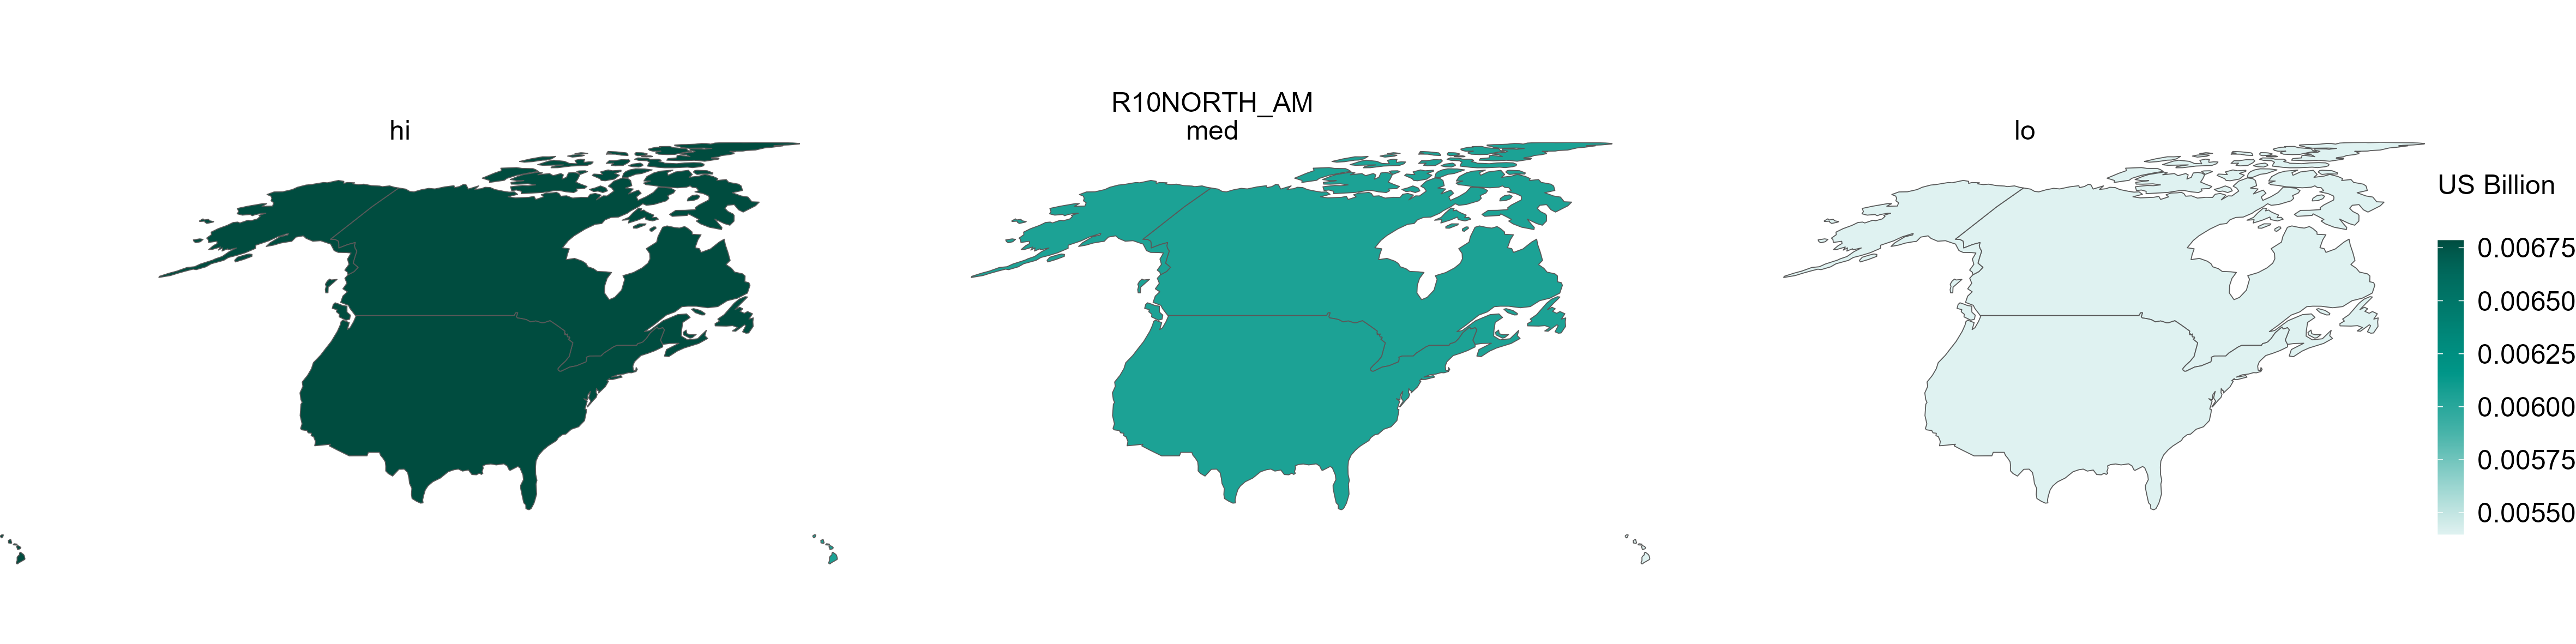
\includegraphics[width=11.5cm]{"Images_meth/damage_NZ/vsl/map_vsl_R10NORTH_AM.png"}};
  \node[draw=white,rectangle,rounded corners] (india_VSL) [below = of northAm_VSL, yshift = 1cm] {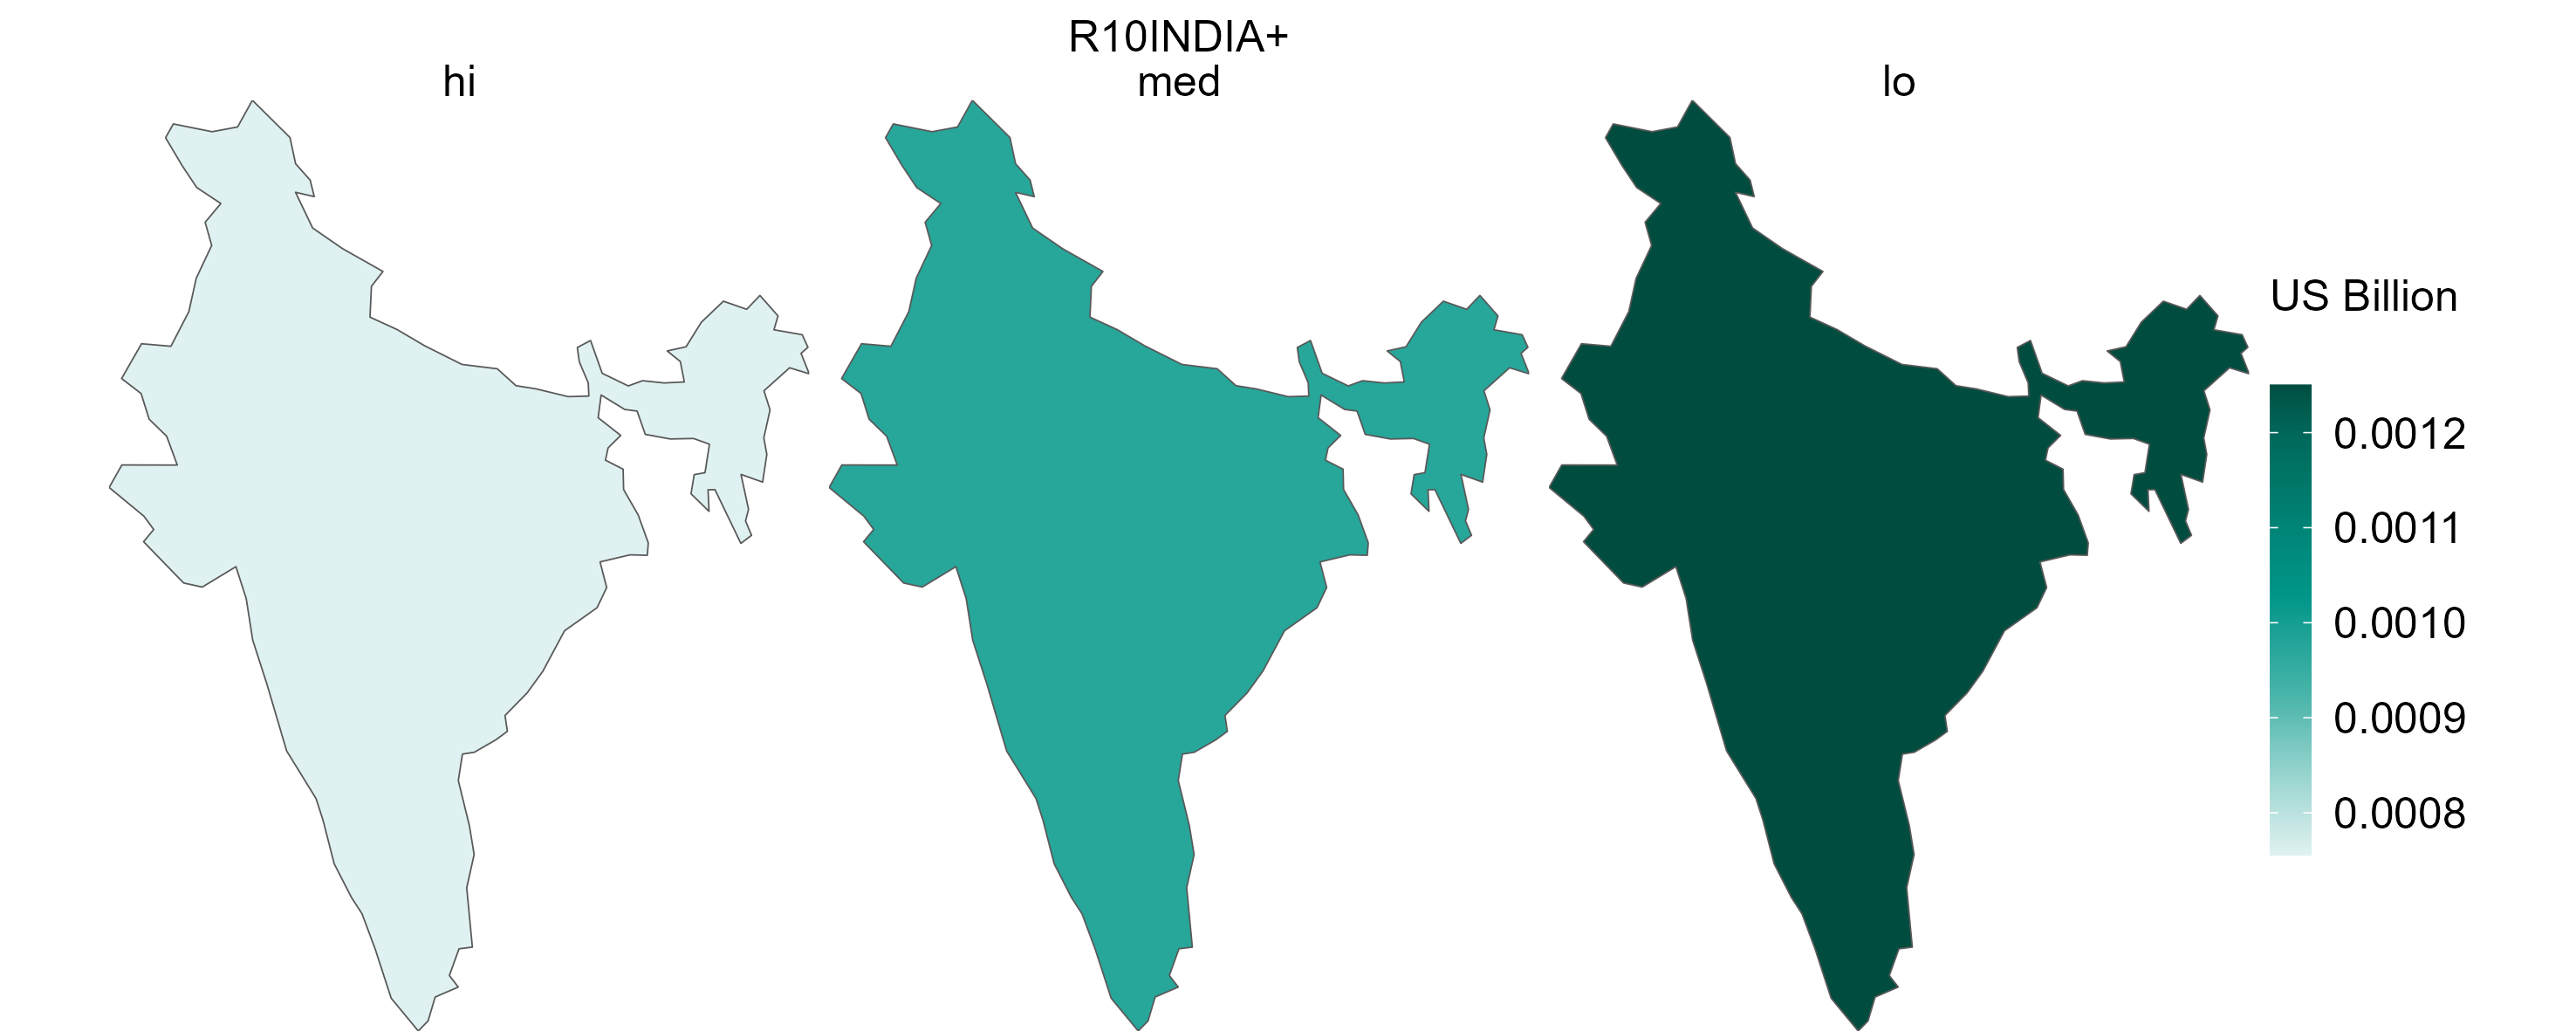
\includegraphics[width=11cm, height=3cm, keepaspectratio=FALSE]{"Images_meth/damage_NZ/vsl/map_vsl_R10INDIA+.png"}};
  \node[draw=white,rectangle,rounded corners] (eqVSLfigs) [above = of northAm_VSL, yshift = -1cm]  {\scalebox{0.7}{$VSL_{i,t} = VSL_{R10EUROPE,2005} \cdot \left(\frac{GDPpc_{i,t}}{GDPpc_{R10EUROPE,2005}} \right) ^ \alpha$}};
\end{tikzpicture}
\end{frame}

\begin{frame}{Value of Statistical Life (VSL)}
  $AvoidedDamage_{i,t,p} = (VSL_{i,t,p} \cdot \tikzmark{premMortVSL} \Delta Mort_{i,t,p}) - (VSL_{i,t,REF} \cdot \Delta Mort_{i,t,REF})$
  \begin{equation*}
    \hspace{10000pt minus 1fil} i \in \{\text{region}\}, t \in \{\text{year}\}, p \in \{\text{policy}\} \hfilneg
  \end{equation*}
  \begin{tikzpicture}[remember picture,overlay]
    \onslide<2->{
    % premature mortality
    \draw[<-] 
      ([shift={(7pt,15pt)}]pic cs:premMortVSL) |- ([shift={(17pt,23pt)}]pic cs:premMortVSL) 
      node[anchor=west] {$\scriptstyle \text{Premature Mortality}$}; 
    \draw[] 
      ([shift={(7pt,15pt)}]pic cs:premMortVSL)  ([shift={(17pt,15pt)}]pic cs:premMortVSL) 
      node[anchor=west] {$\scriptstyle \text{due to \pmm\ \& \oo}$}; }
  \end{tikzpicture}
\end{frame}  

\begin{frame}{Value of Statistical Life (VSL)}
  \centering
  \begin{tikzpicture}
    \centering
    \node[draw=white,rectangle,rounded corners] at (0,0) (northAm_VSL) {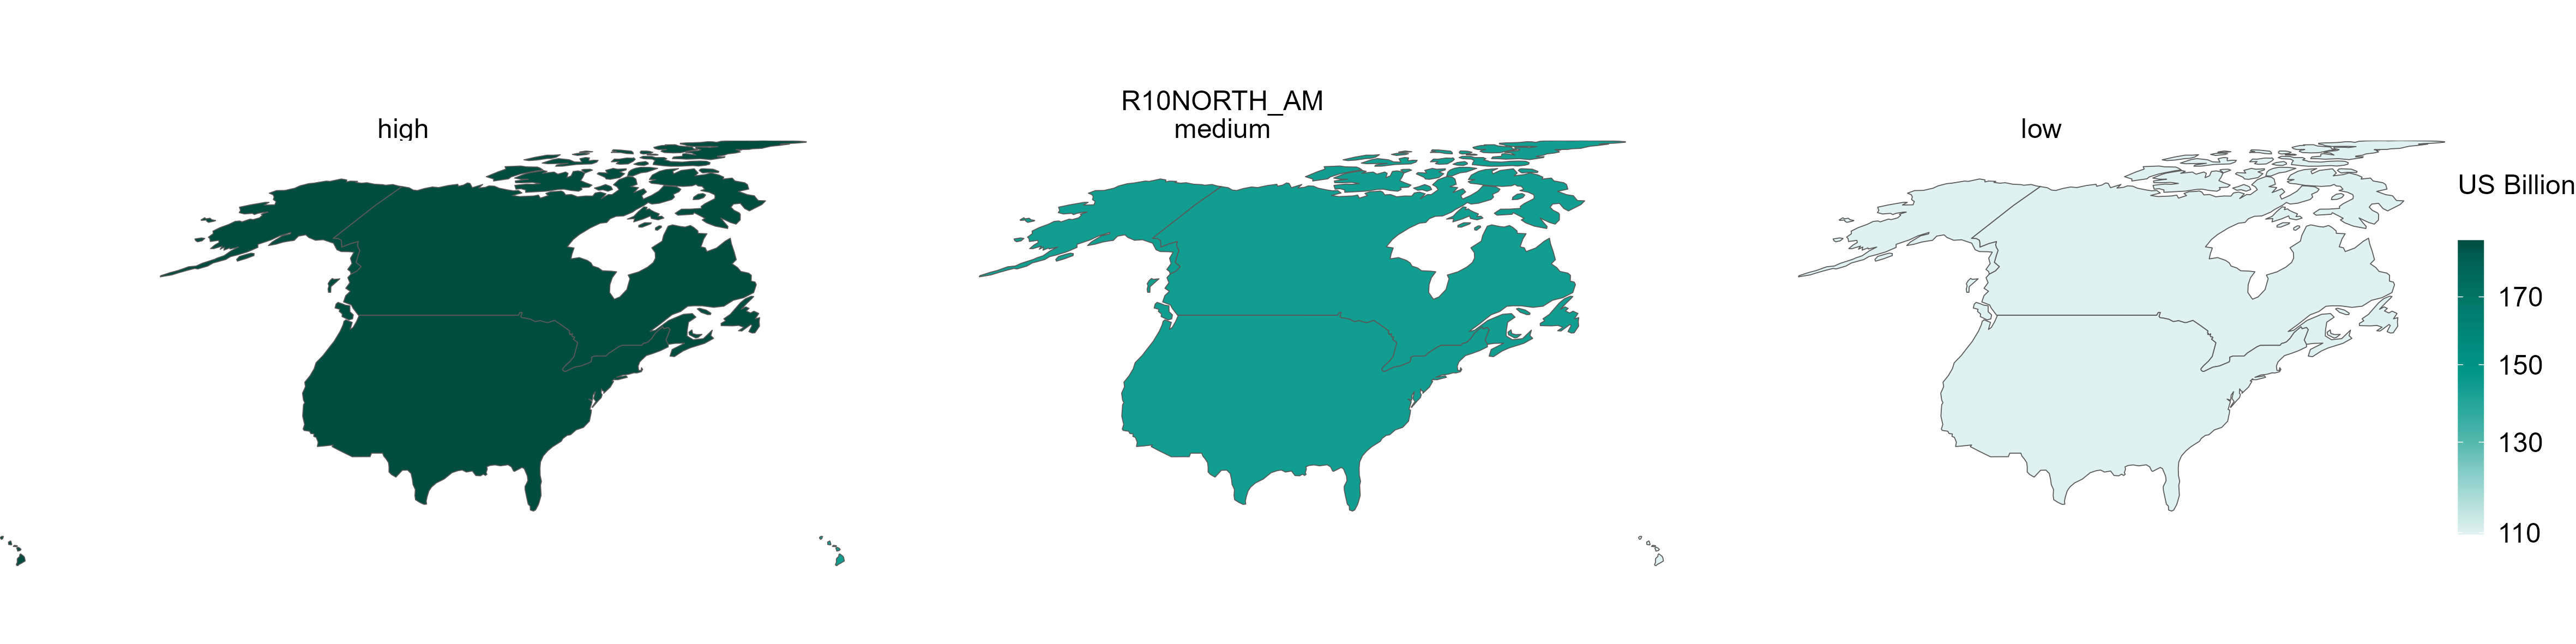
\includegraphics[width=11.5cm]{"Images_meth/damage_NZ/vsl_NZ_median/map_vsl_NZ_median_R10NORTH_AM.png"}};
    \node[draw=white,rectangle,rounded corners] (india_VSL) [below = of northAm_VSL, yshift = 1cm] {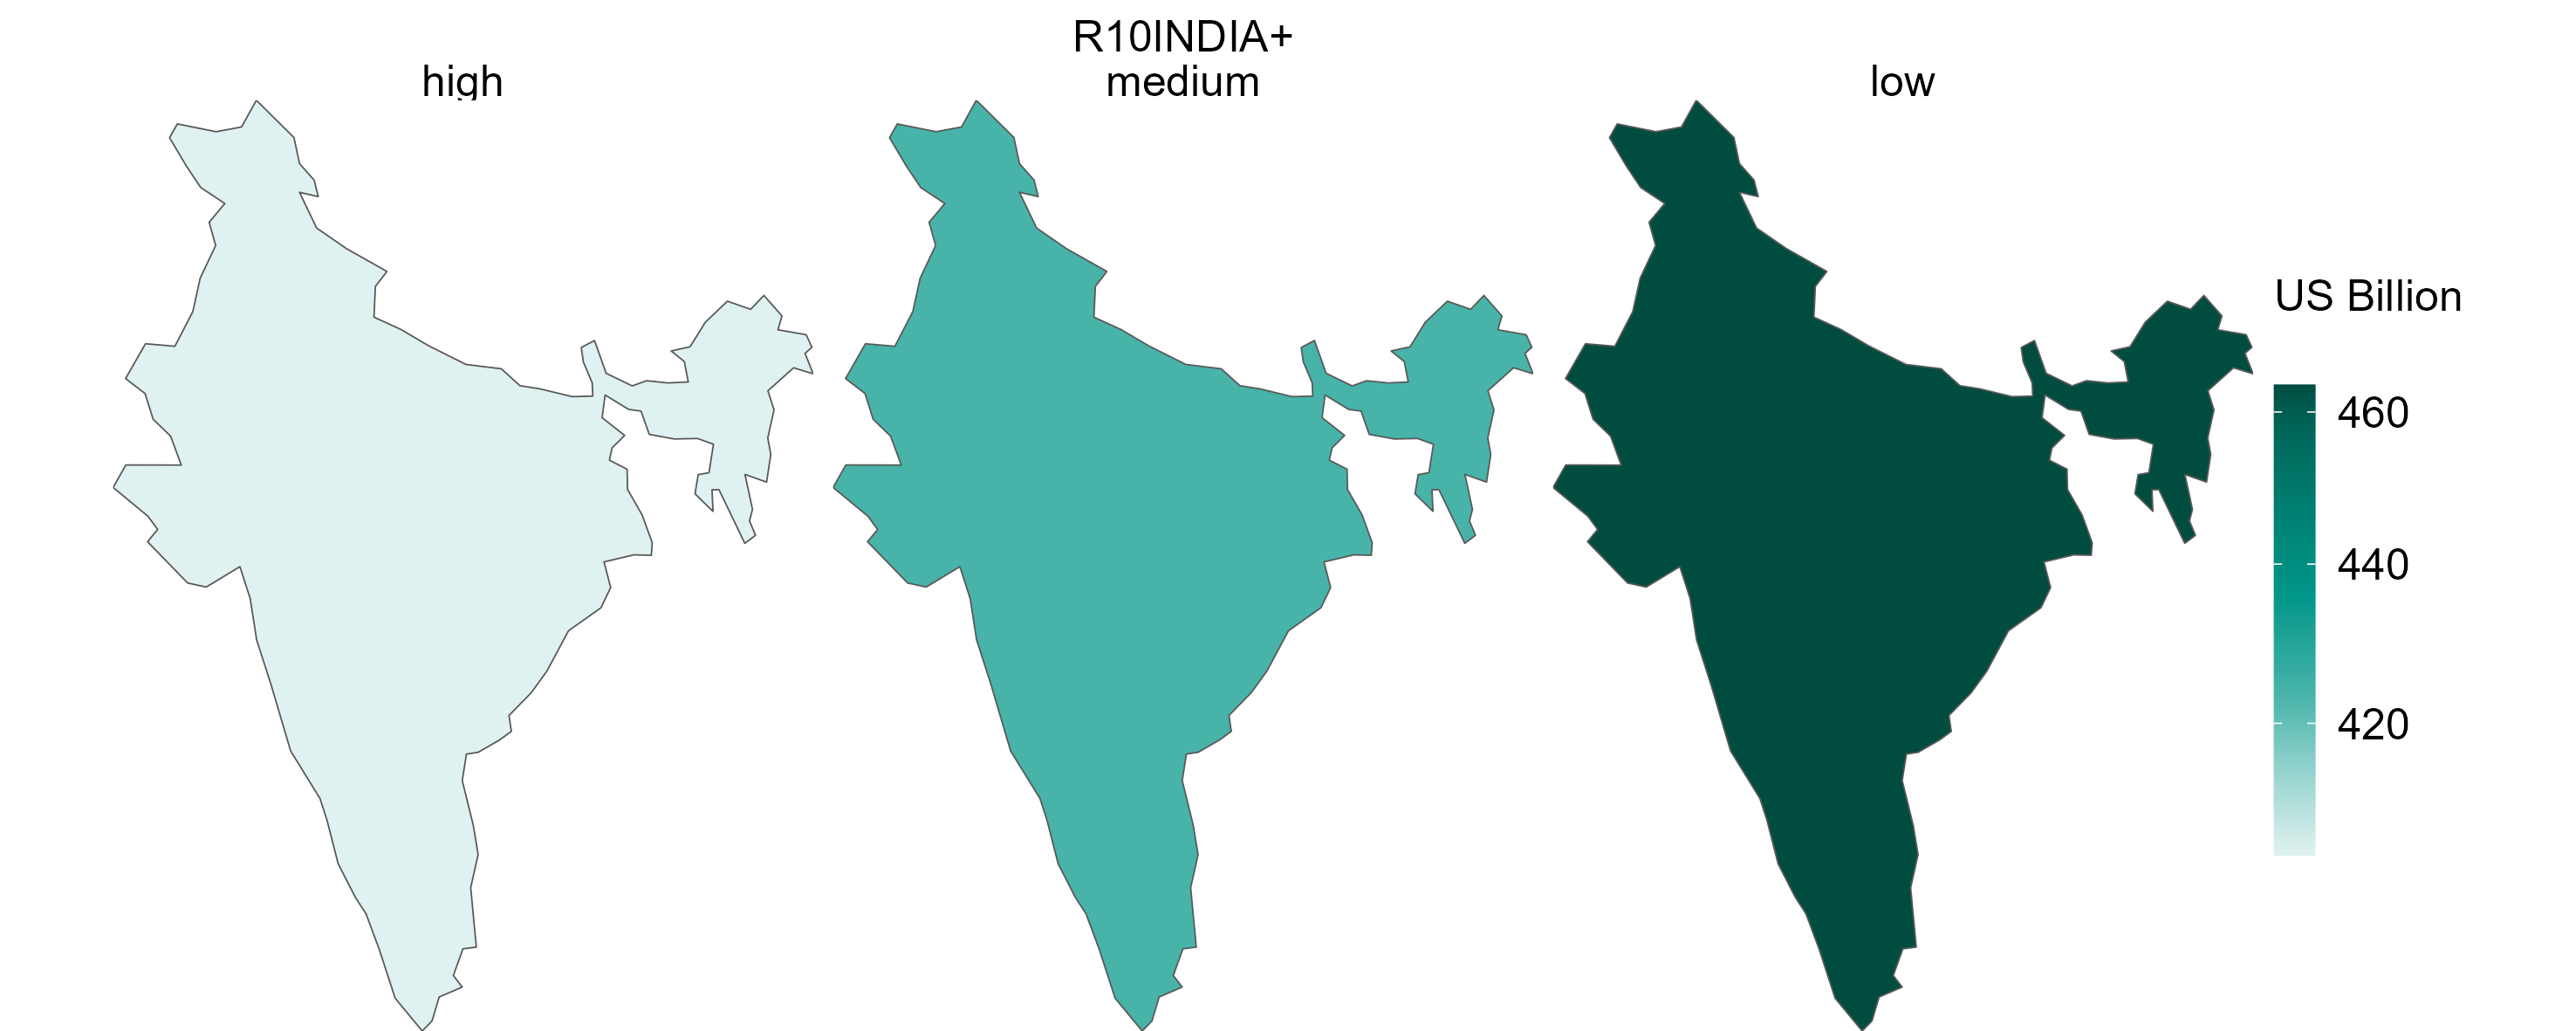
\includegraphics[width=11cm, height=3cm, keepaspectratio=FALSE]{"Images_meth/damage_NZ/vsl_NZ_median/map_vsl_NZ_median_R10INDIA+.png"}};
    \node[draw=white,rectangle,rounded corners] (eqVSLfigs) [above = of northAm_VSL, yshift = -1cm]  {\scalebox{0.7}{$AvoidedDamage_{i,t,p} = (VSL_{i,t,p} \cdot \tikzmark{premMortVSL} \Delta Mort_{i,t,p}) - (VSL_{i,t,REF} \cdot \Delta Mort_{i,t,REF})$}};
  \end{tikzpicture}
\end{frame}
  

\begin{frame}{Value of Statistical Life (VSL)}
  \centering
  \begin{tikzpicture}
    \centering
    \node[draw=white,rectangle,rounded corners] at (0,0) (northAm_VSL2) {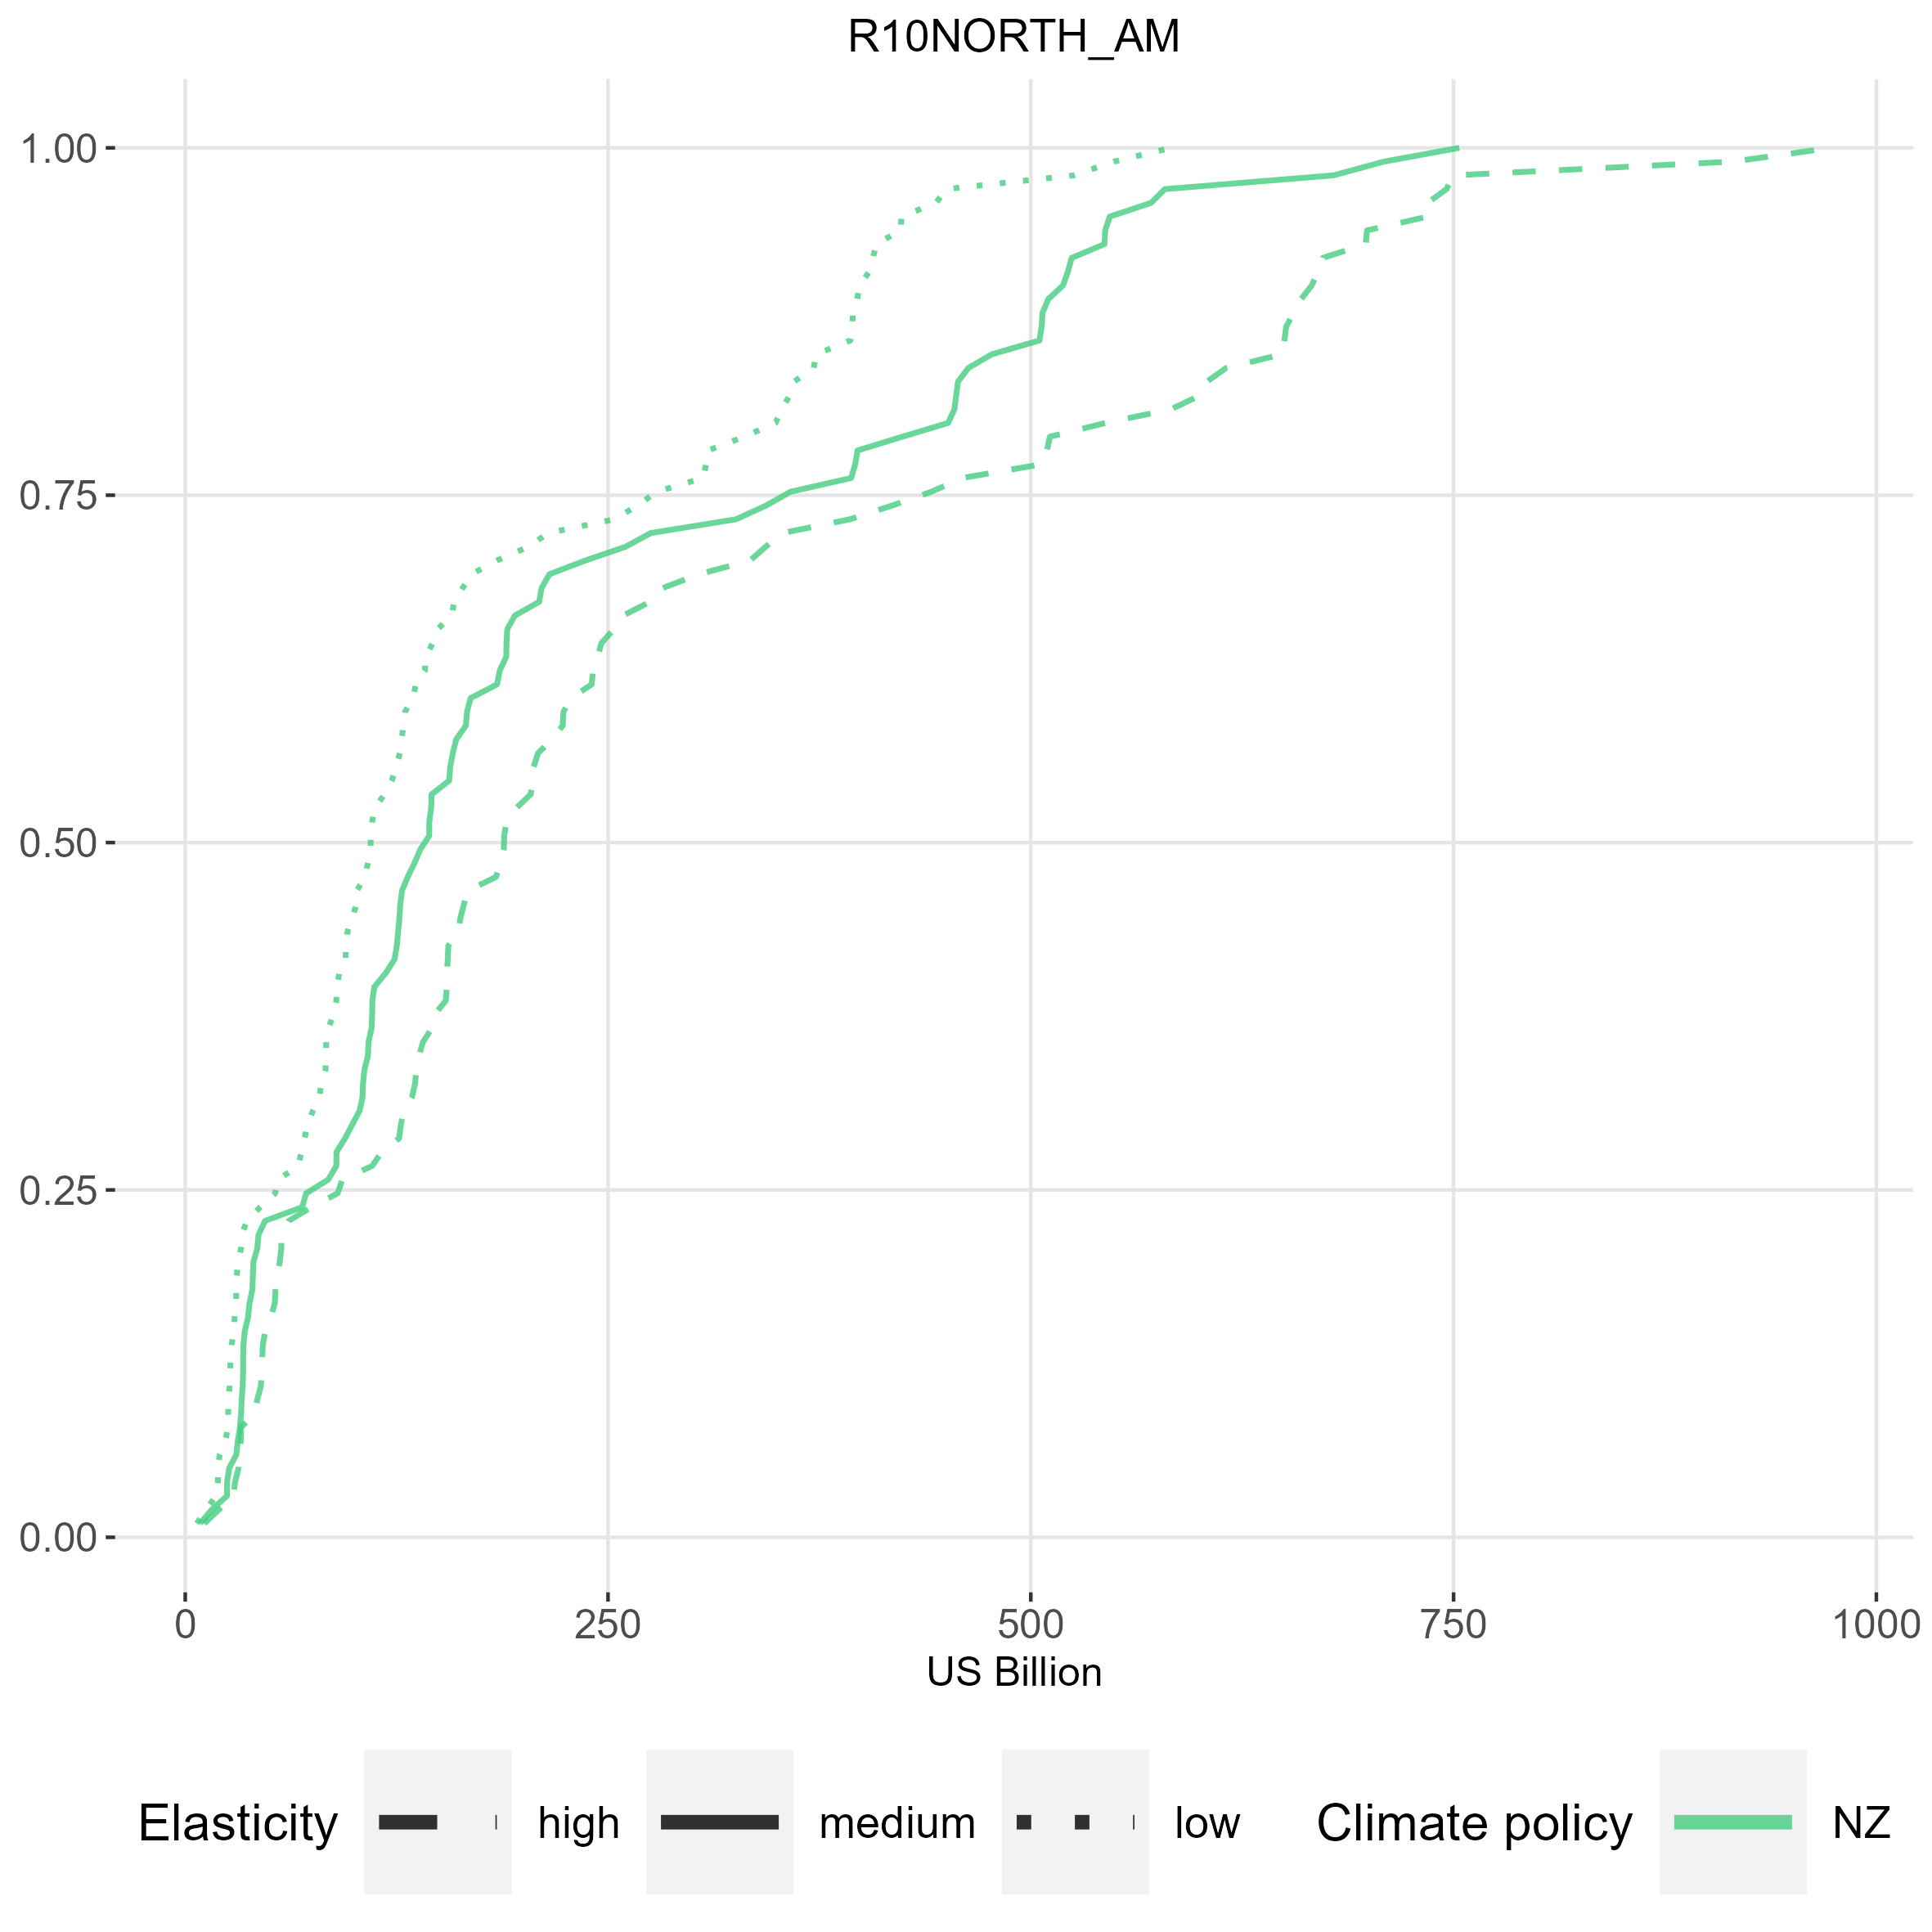
\includegraphics[width=5cm]{"Images_meth/damage_NZ/vsl_NZ_median/cum_freq_vsl_NZ_median_R10NORTH_AM.png"}};
    \node[draw=white,rectangle,rounded corners] (india_VSL2) [right = of northAm_VSL2] {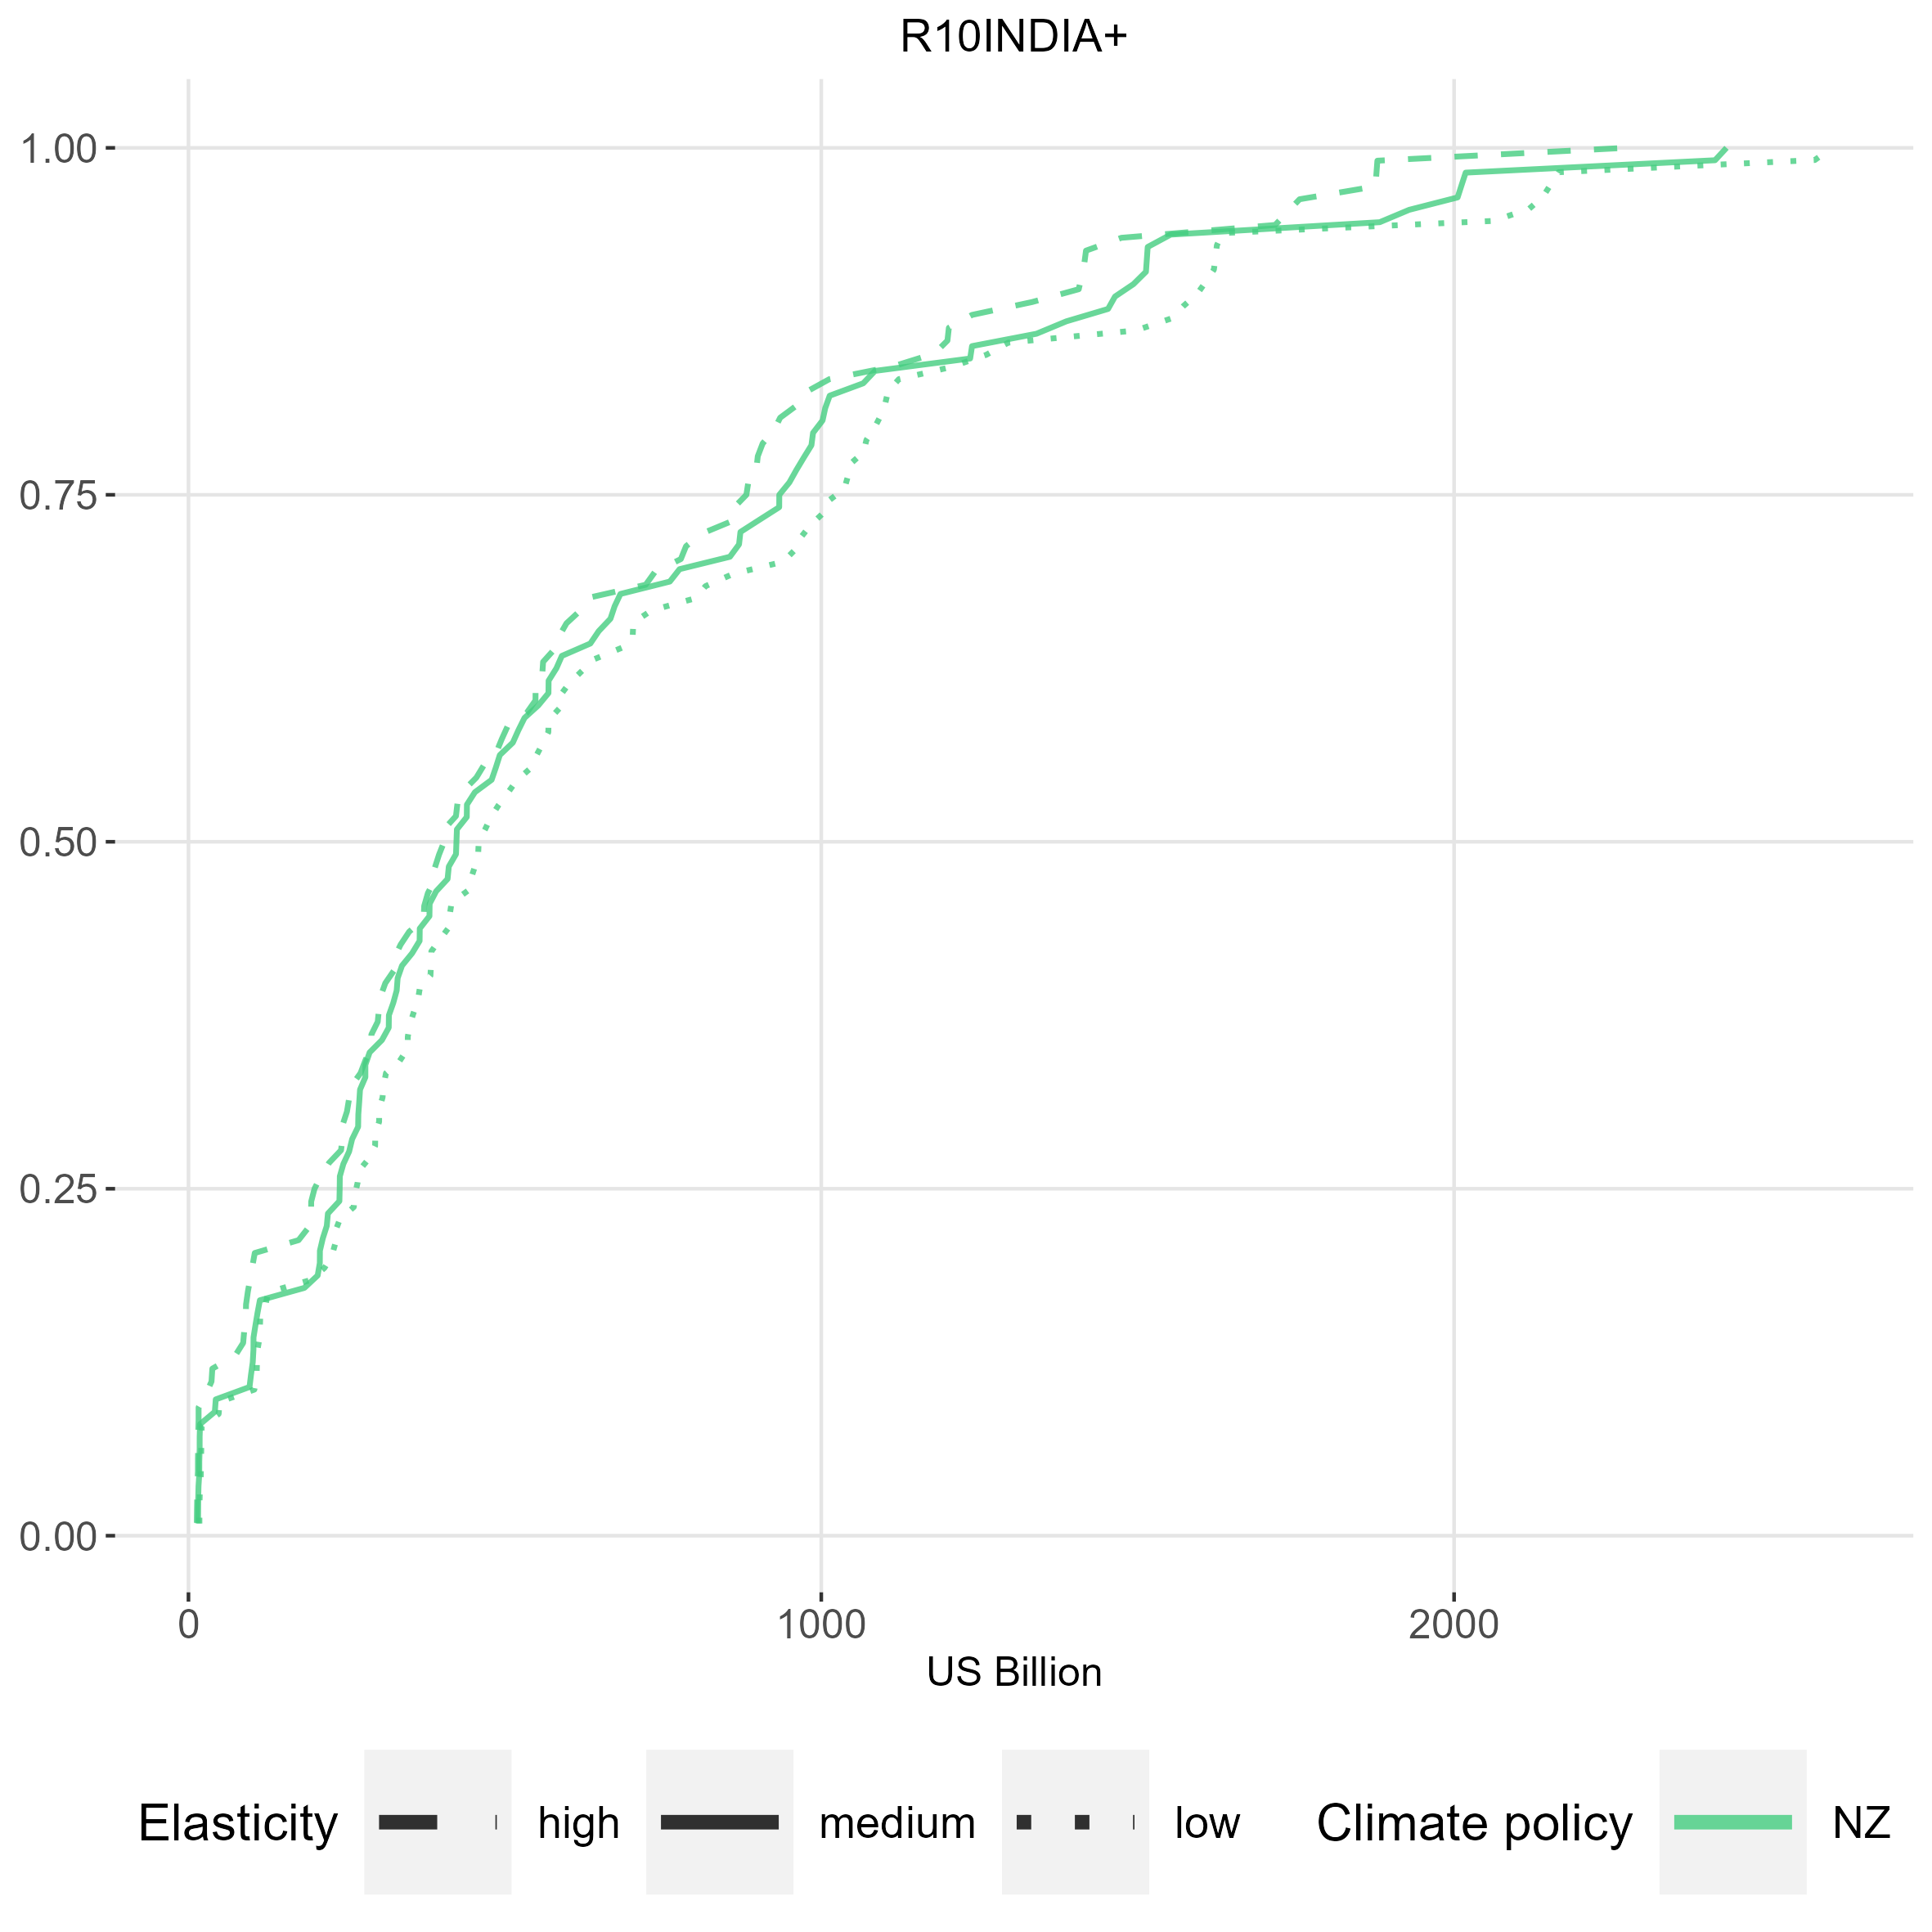
\includegraphics[width=5cm]{"Images_meth/damage_NZ/vsl_NZ_median/cum_freq_vsl_NZ_median_R10INDIA+.png"}};
    \node[draw=white,rectangle,rounded corners] (eqVSLfigs) [above = of northAm_VSL2, xshift = 3cm, yshift = -1cm]  {\scalebox{0.7}{$AvoidedDamage_{i,t,p} = (VSL_{i,t,p} \cdot \tikzmark{premMortVSL} \Delta Mort_{i,t,p}) - (VSL_{i,t,REF} \cdot \Delta Mort_{i,t,REF})$}};
  \end{tikzpicture}
\end{frame}
  
% Human Capital Loss %------------------------------------------------%------------------------------------------------%------------------------------------------------
\begin{frame}{Human Capital Loss (HCL)}
% It refers to the loss of human capital
% due to severe illness or premature death due to PM2.5 pollution
$$HCL_{i,t} = \tikzmark{hc1}HC_{i,t} \cdot \tikzmark{delta}\Delta Mort_{i,t}$$
\onslide<3->{
where,
$$\tikzmark{hc}HC_{i,t} = \sum_{i=1}^t GDP_{i,t} \cdot \left(\frac{1+\tikzmark{gamma}\gamma}{1+\tikzmark{alpha}\alpha}\right), \; \; \alpha \in \{0.6, 0.8, 1\}$$
\begin{equation*}
    \hspace{10000pt minus 1fil} i \in \{\text{region}\} \hfilneg
\end{equation*}
\begin{equation*}
    \hspace{10000pt minus 1fil} t \in \{\text{year}\} \hfilneg
\end{equation*}
}
\begin{tikzpicture}[remember picture,overlay]
% human capital
\onslide<2->{
\draw[<-] 
  ([shift={(5pt,15pt)}]pic cs:hc1) |- ([shift={(15pt,23pt)}]pic cs:hc1) 
  node[anchor=west] {$\scriptstyle \text{Human}$}; 
\draw[] 
  ([shift={(5pt,15pt)}]pic cs:hc1)  ([shift={(15pt,15pt)}]pic cs:hc1) 
  node[anchor=west] {$\scriptstyle \text{Capital}$}; 
% premature mortality
\draw[<-] 
  ([shift={(20pt,15pt)}]pic cs:delta) |- ([shift={(30pt,23pt)}]pic cs:delta) 
  node[anchor=west] {$\scriptstyle \text{Premature Mortality}$}; 
\draw[] 
  ([shift={(20pt,15pt)}]pic cs:delta)  ([shift={(30pt,15pt)}]pic cs:delta) 
  node[anchor=west] {$\scriptstyle \text{due to \pmm,\ adults}$}; }
% GDP annual growth
\onslide<4->{
\draw[<-] 
  ([shift={(4.5pt,8pt)}]pic cs:gamma) |- ([shift={(16pt,16pt)}]pic cs:gamma) 
  node[anchor=west] {$\scriptstyle \text{GDP annual growth}$}; 
% elasticity
\draw[<-] 
  ([shift={(4.5pt,-6pt)}]pic cs:alpha) |- ([shift={(16pt,-14pt)}]pic cs:alpha) 
  node[anchor=west] {$\scriptstyle \text{elasticity}$}; 
% human capital
\draw[<-] 
  ([shift={(8pt,-10pt)}]pic cs:hc) |- ([shift={(8pt,-20pt)}]pic cs:hc) 
  node[anchor=north] {$\scriptstyle \text{Human Capital}$}; 
  }
\end{tikzpicture}
\vfill \hfill \cite{liu_monitoring_2011,zhao_impact_2022}
\end{frame}

\begin{frame}{Human Capital Loss (HCL)}
  $AvoidedDamage_{i,t,p} = (GDP_{i,t,REF} - HCL_{i,t,REF}) - (GDP_{i,t,p} - HCL_{i,t,p})$
  \begin{equation*}
    \hspace{10000pt minus 1fil} i \in \{\text{region}\}, t \in \{\text{year}\}, p \in \{\text{policy}\} \hfilneg
  \end{equation*}
\end{frame}

\begin{frame}{Human Capital Loss (HCL)}
  \centering
  \begin{tikzpicture}
    \centering
    \node[draw=white,rectangle,rounded corners] at (0,0) (northAm_hcl) {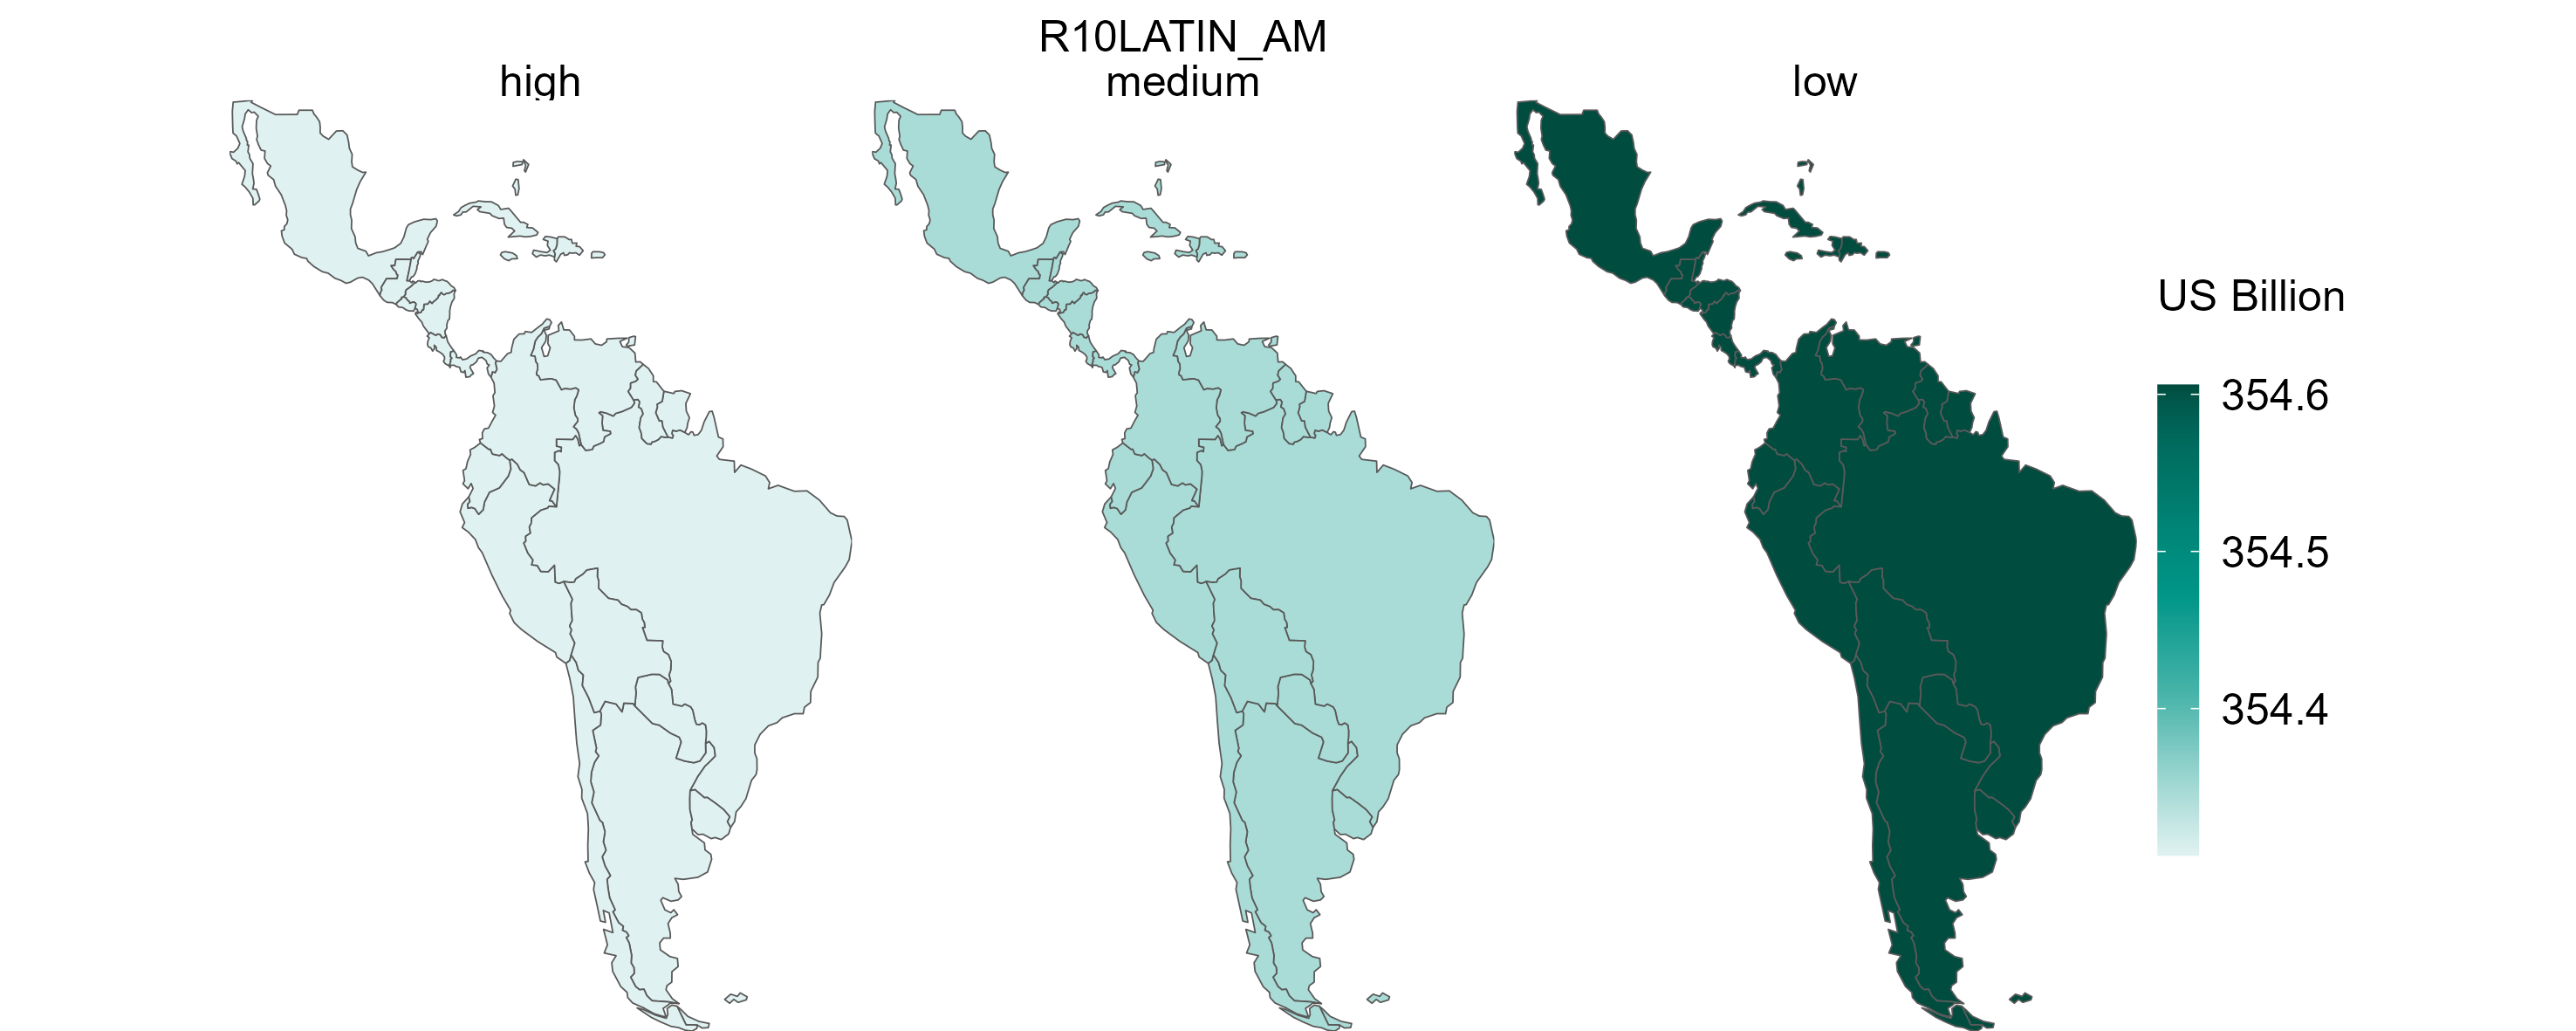
\includegraphics[width=13cm, height=3cm, keepaspectratio=FALSE]{"Images_meth/damage_NZ/hcl_NZ_median/map_hcl_NZ_median_R10LATIN_AM.png"}};
    \node[draw=white,rectangle,rounded corners] (india_hcl) [below = of northAm_hcl, yshift = 1cm] {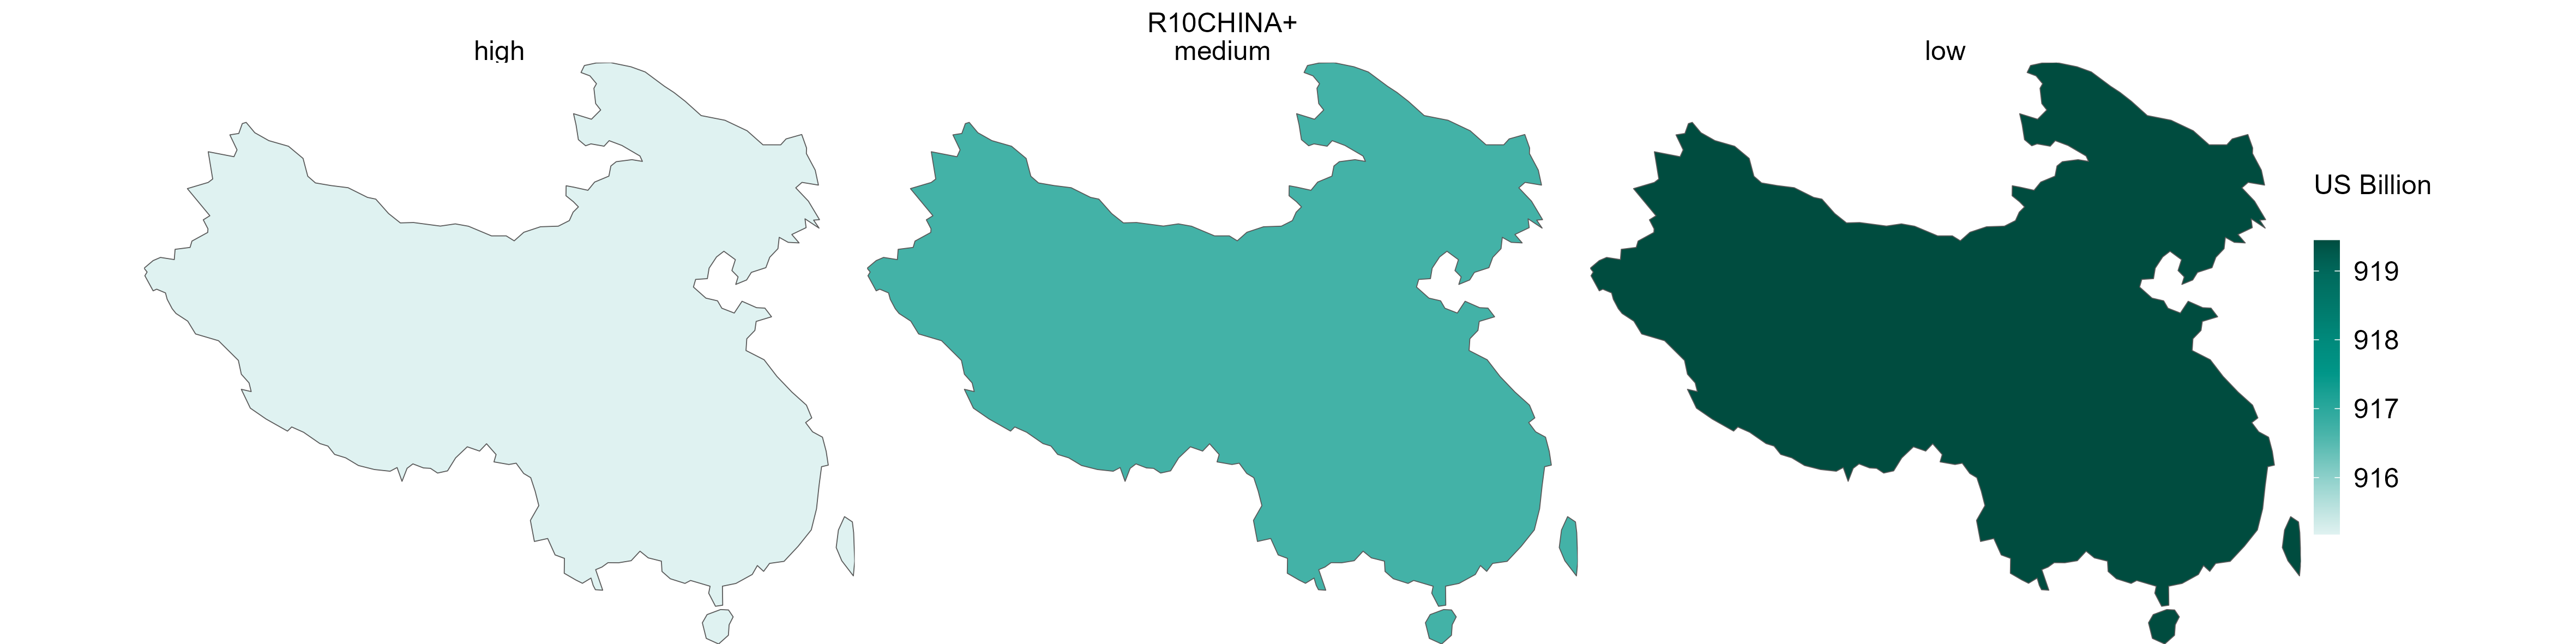
\includegraphics[width=11cm]{"Images_meth/damage_NZ/hcl_NZ_median/map_hcl_NZ_median_R10CHINA+.png"}};
    \node[draw=white,rectangle,rounded corners] (eqhclfigs) [above = of northAm_hcl, yshift = -0.5cm]  {\scalebox{0.7}{$AvoidedDamage_{i,t,p} = (GDP_{i,t,REF} - HCL_{i,t,REF}) - (GDP_{i,t,p} - HCL_{i,t,p})$}};
  \end{tikzpicture}
  \end{frame}
  
  \begin{frame}{Human Capital Loss (HCL)}
    \centering
    \begin{tikzpicture}
      \centering
      \node[draw=white,rectangle,rounded corners] at (0,0) (northAm_hcl2) {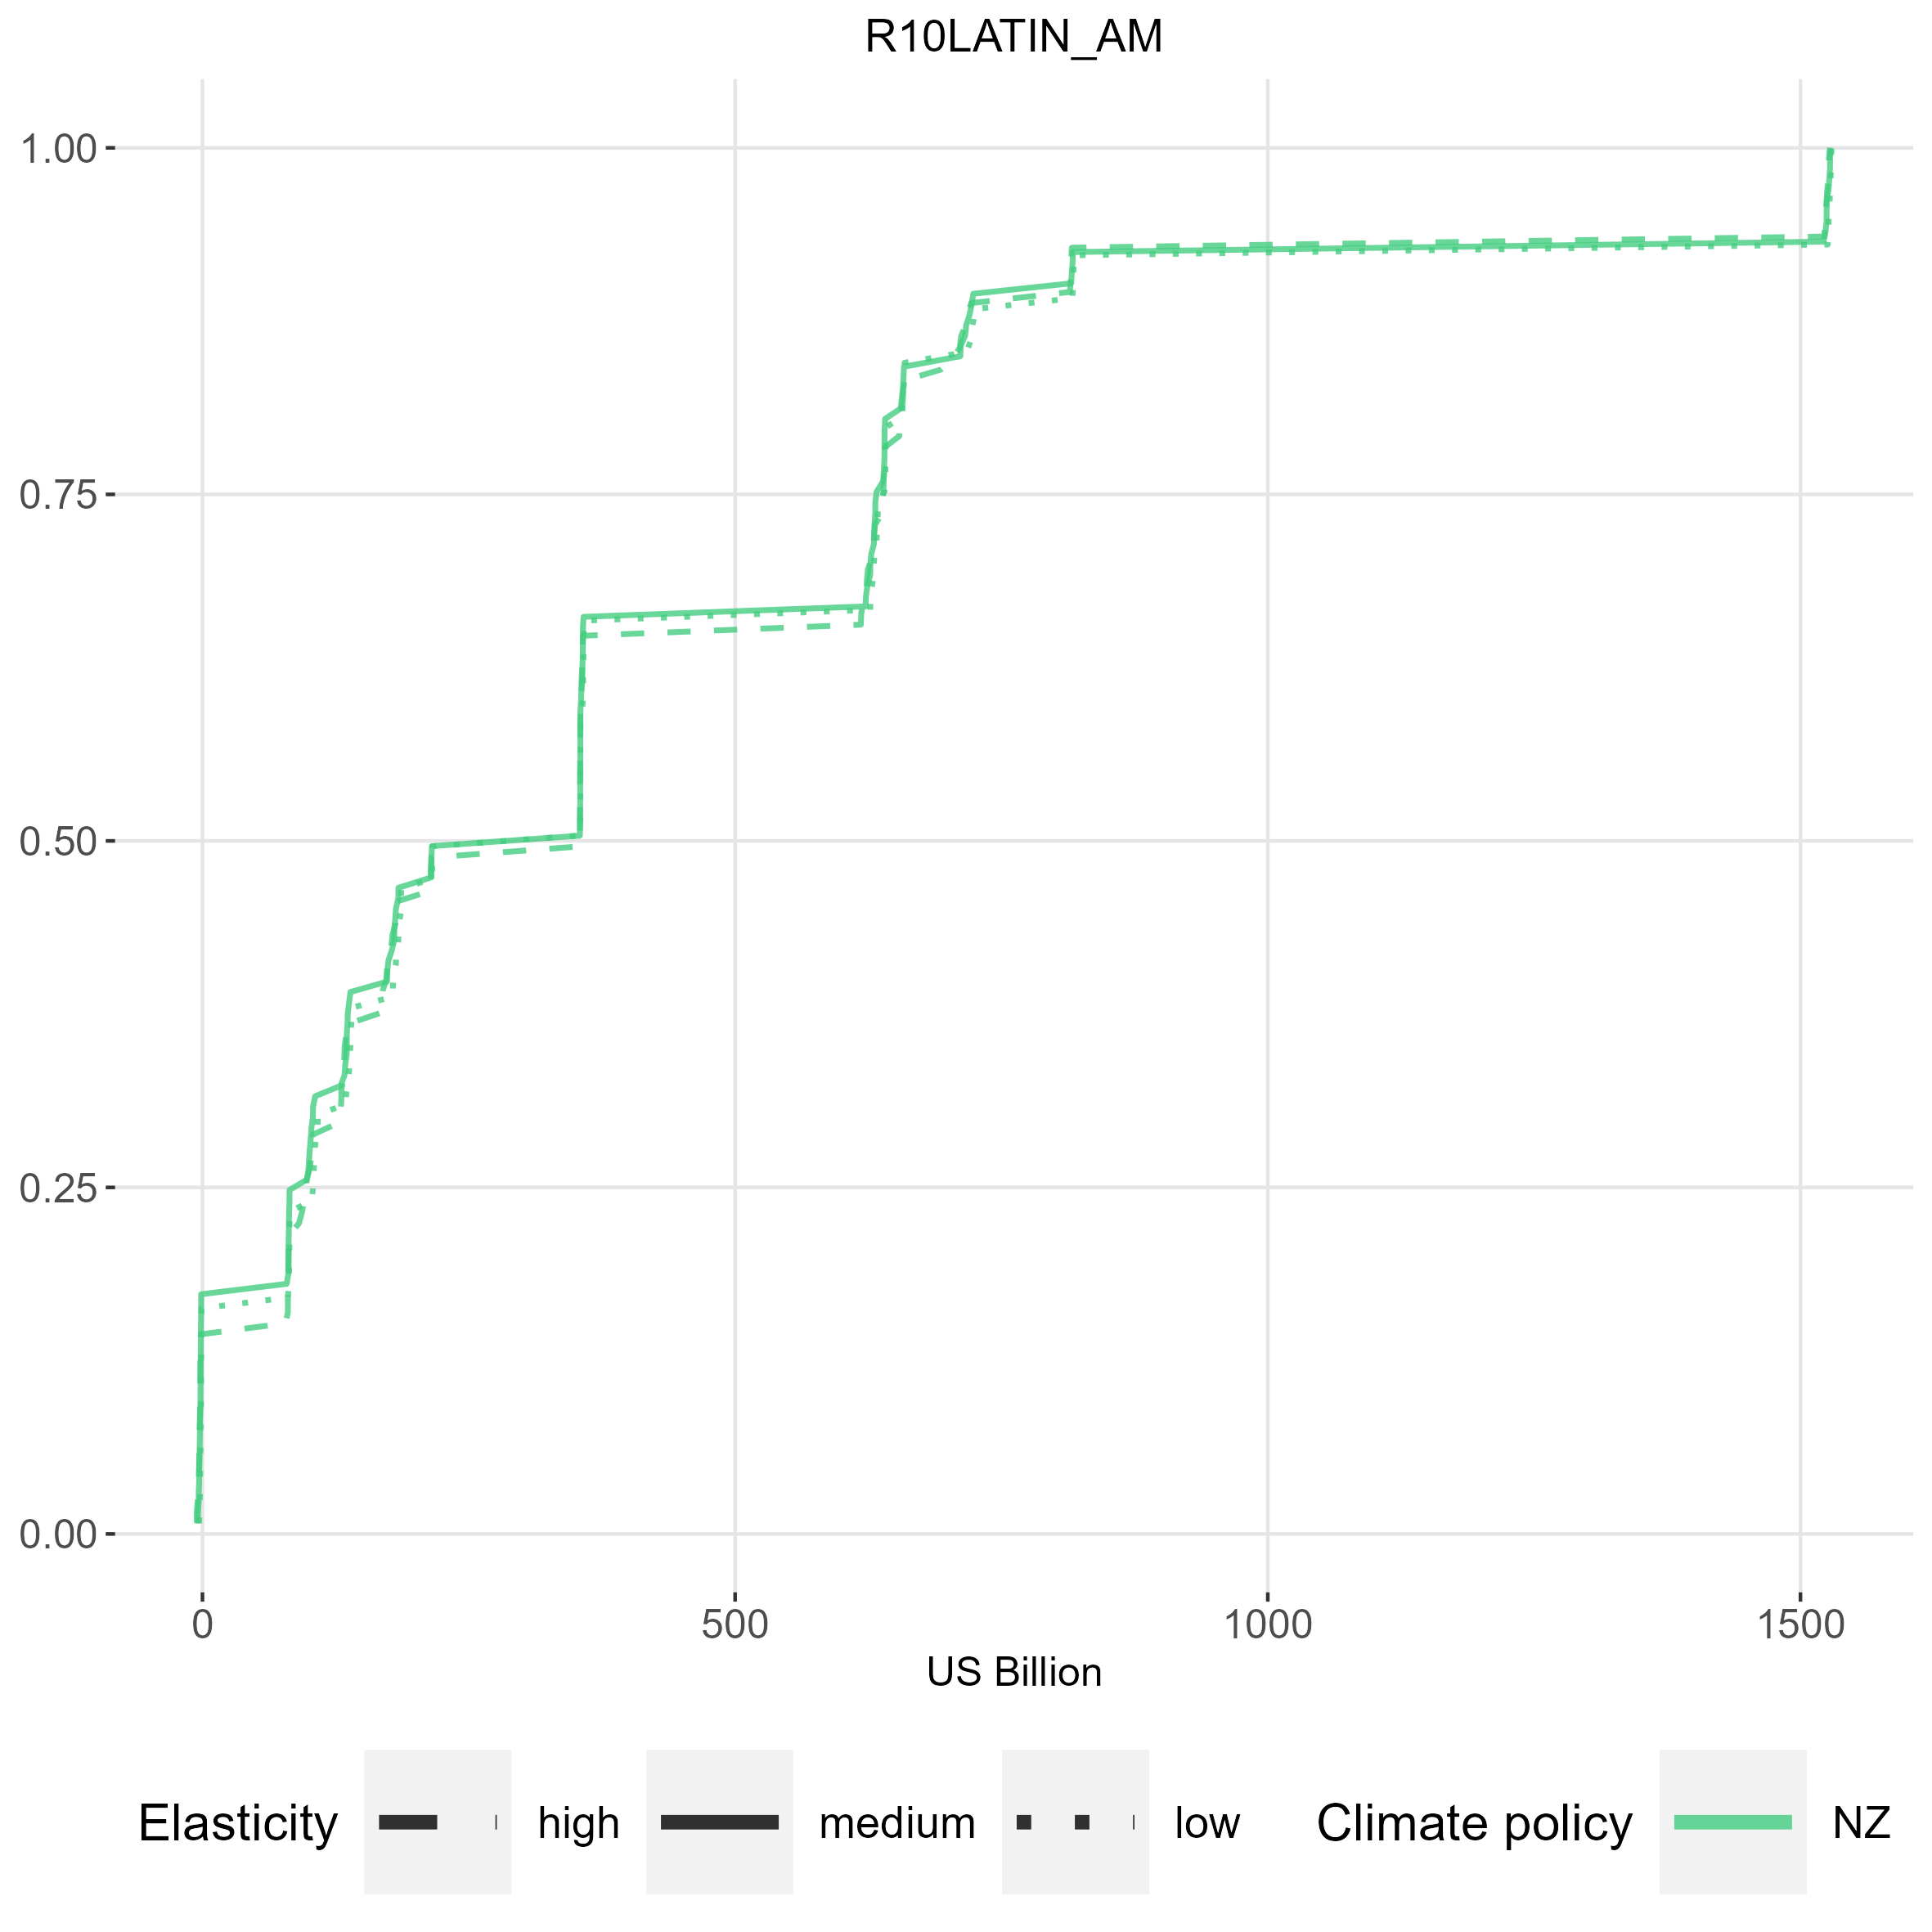
\includegraphics[width=5cm]{"Images_meth/damage_NZ/hcl_NZ_median/cum_freq_hcl_NZ_median_R10LATIN_AM.png"}};
      \node[draw=white,rectangle,rounded corners] (india_hcl2) [right = of northAm_hcl2] {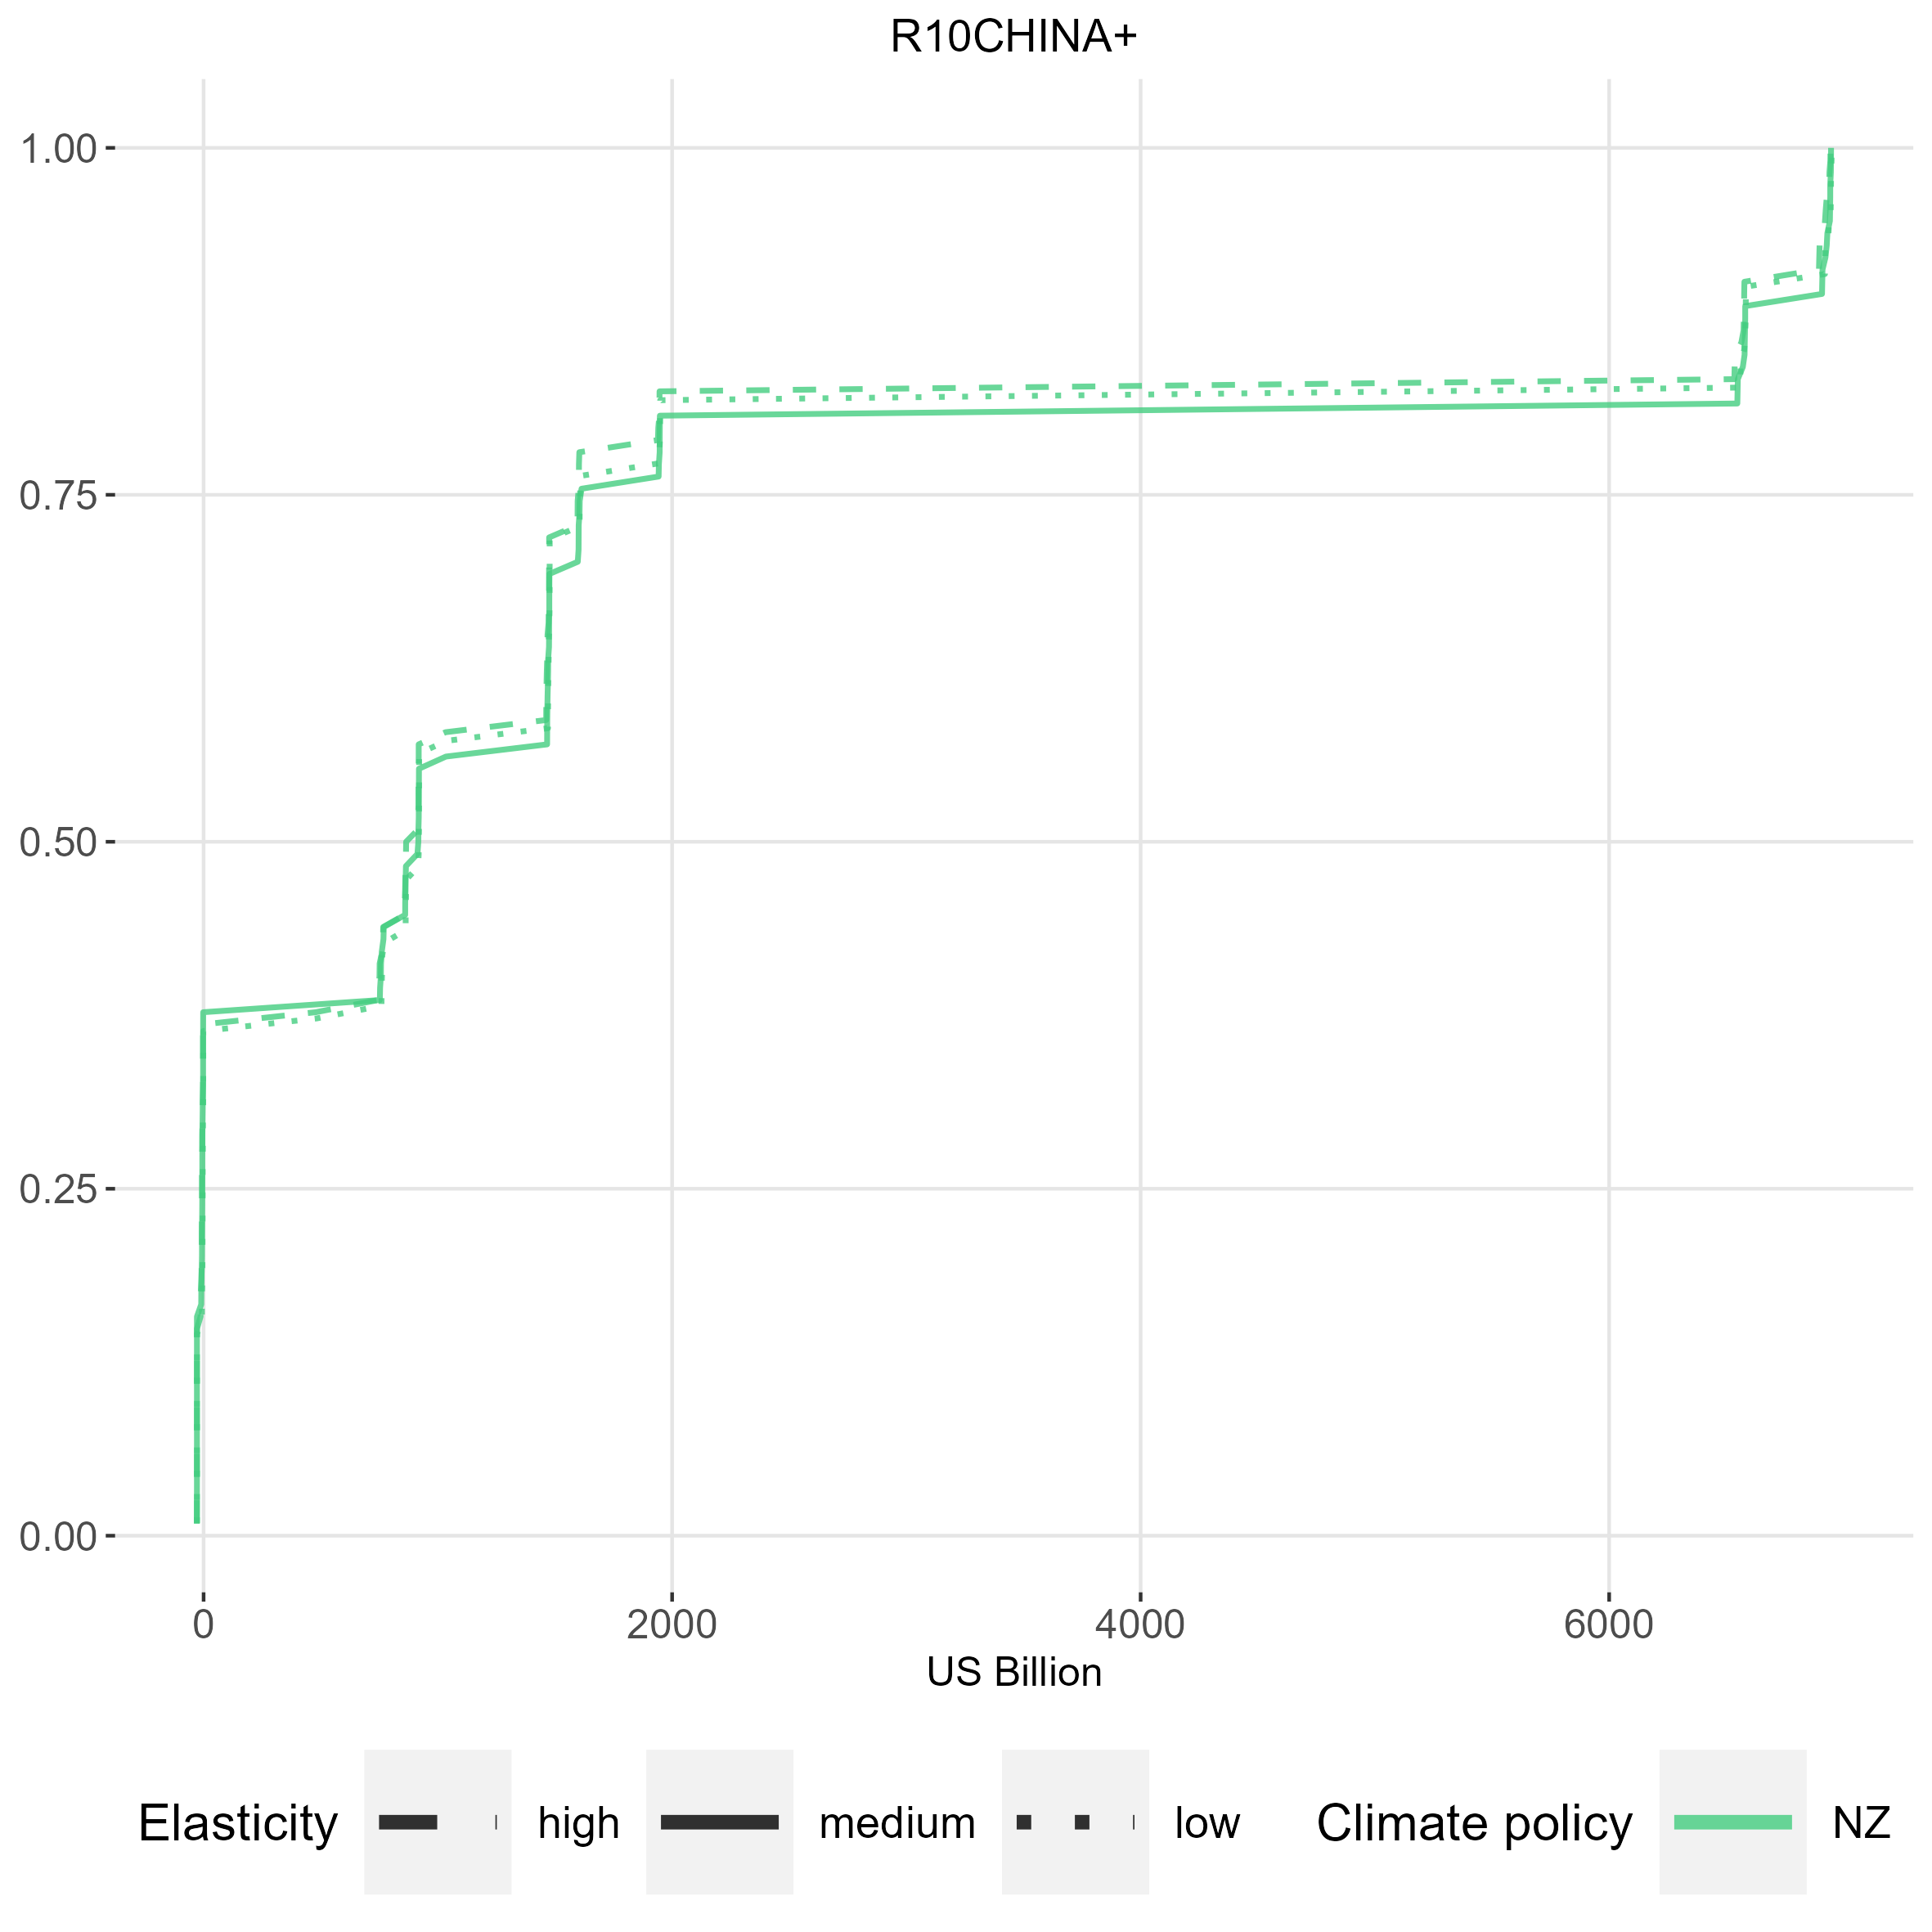
\includegraphics[width=5cm]{"Images_meth/damage_NZ/hcl_NZ_median/cum_freq_hcl_NZ_median_R10CHINA+.png"}};
      \node[draw=white,rectangle,rounded corners] (eqhclfigs) [above = of northAm_hcl2, xshift = 3cm, yshift = -1cm]  {\scalebox{0.7}{$AvoidedDamage_{i,t,p} = (GDP_{i,t,REF} - HCL_{i,t,REF}) - (GDP_{i,t,p} - HCL_{i,t,p})$}};
    \end{tikzpicture}
  \end{frame}
  

% Dechezleprêtre et al. 2019 %------------------------------------------------%------------------------------------------------%------------------------------------------------

\begin{frame}{Dechezleprêtre et al. 2019}
% Recently,Dechezleprêtreetal.[10]established an econometric model with data from the European region. It focuses on the impact of air pollution on the GDP value per capita. It considers some other factors, such as weather covariates and thermal inversions, which have been wiped off for our purpose. Thus, the equation is simply
$$\tikzmark{GDPiniDech} \Delta \tikzmark{GDP} ln GDP{i,t} = \gamma_{1} \tikzmark{APDech} \Delta AP_{i,t} + \gamma_{2} \tikzmark{flexfun} \Delta f(W_{i,t}) + \Delta \tikzmark{region-year-effects} \nu_{i,t} + \Delta \tikzmark{errorDech} \varepsilon_{i,t}$$
\vspace{0.5cm}
\only<1-2>{
    \begin{equation*}
        \hspace{10000pt minus 1fil} i \in \{\text{region}\} \hfilneg
    \end{equation*}
    \begin{equation*}
        \hspace{10000pt minus 1fil} t \in \{\text{year}\} \hfilneg
    \end{equation*}
}
\onslide<3-7>{
    \begin{equation*}
        \hspace{10000pt minus 1fil} i \in \text{ region,} \; t \in \{\text{year}\} \hfilneg
    \end{equation*}
}

% gamma can be interpreted as the contemporaneous growth rate of GDP stemming from a one-unit increase in the pollution concentration
\onslide<3-7>{$$\tikzmark{GDPsimplifiedDech} \Delta ln GDP_{i,t} = \tikzmark{gg}\gamma_{i,t} \Delta AP_{i,t}$$ }

\only<4-5>{$$\Delta ln GDP_{i,t} = ln GDP_{i,t,p1} - ln GDP_{i,t,p2} \tikzmark{taylor}\approx \frac{ln GDP_{i,t,p1} - ln GDP_{i,t,p2}}{ln GDP_{i,t,p2}}$$ }

\onslide<6-7>{$$\gamma_{i,t} = \gamma_{R10EUROPE, 2015} \cdot \left(\frac{GDPpc_{i,t}}{GDPpc_{R10EUROPE,2015}}\right)^\alpha\tikzmark{elasticityDech}, \; \; \alpha \in \{0.8, 1, 1.2\}$$ }

\begin{tikzpicture}[remember picture,overlay]
% GDP per capita
\onslide<2-7>{
\draw[<-] 
  ([shift={(14pt,15pt)}]pic cs:GDP) |- ([shift={(24pt,23pt)}]pic cs:GDP) 
  node[anchor=west] {$\scriptstyle \text{GDP per capita}$}; 
% air pollution
\draw[<-] 
  ([shift={(7pt,-10pt)}]pic cs:APDech) |- ([shift={(17pt,-18pt)}]pic cs:APDech) 
  node[anchor=west] {$\scriptstyle \text{\pmm}$}; 
\draw[] 
  ([shift={(7pt,-10pt)}]pic cs:APDech)  ([shift={(16pt,-23pt)}]pic cs:APDech) 
  node[anchor=west] {$\scriptstyle \text{concentration}$}; 
% flexible function: captures how the economic output may be affected by weather (temperature, precipitation, humidity, atmospheric pressure, wind speed, etc.)
\draw[<-] 
  ([shift={(14pt,15pt)}]pic cs:flexfun) |- ([shift={(24pt,23pt)}]pic cs:flexfun) 
  node[anchor=west] {$\scriptstyle \text{flexible}$}; 
\draw[] 
  ([shift={(14pt,15pt)}]pic cs:flexfun)  ([shift={(23pt,15pt)}]pic cs:flexfun) 
  node[anchor=west] {$\scriptstyle \text{function}$}; 
% fixed region - year effects
\draw[<-] 
  ([shift={(5pt,-10pt)}]pic cs:region-year-effects) |- ([shift={(15pt,-18pt)}]pic cs:region-year-effects) 
  node[anchor=west] {$\scriptstyle \text{fixed region-year}$}; 
\draw[] 
  ([shift={(5pt,-25pt)}]pic cs:region-year-effects) ([shift={(15pt,-25pt)}]pic cs:region-year-effects) 
  node[anchor=west] {$\scriptstyle \text{effects}$}; 
% error
\draw[<-] 
  ([shift={(5pt,15pt)}]pic cs:errorDech) |- ([shift={(15pt,23pt)}]pic cs:errorDech) 
  node[anchor=west] {$\scriptstyle \text{random}$}; 
\draw[] 
  ([shift={(5pt,7pt)}]pic cs:errorDech)  ([shift={(15pt,15pt)}]pic cs:errorDech) 
  node[anchor=west] {$\scriptstyle \text{disturbance}$}; 
\draw[] 
  ([shift={(5pt,0pt)}]pic cs:errorDech)  ([shift={(15pt,8pt)}]pic cs:errorDech) 
  node[anchor=west] {$\scriptstyle \text{term}$}; 
}
% taylor
\only<4-5>{\draw[<-] ([shift={(6pt,13pt)}]pic cs:taylor) |- ([shift={(6pt,25pt)}]pic cs:taylor) 
node[anchor=south] {$\scriptstyle \text{Taylor aproximation}$}; }
% arrow
\onslide<3-7>{\draw [->,black] (pic cs:GDPiniDech) to [out=200,in=-150] node {} (pic cs:GDPsimplifiedDech);}
% circle around gamma
\onslide<5-7>{\draw[red] ([xshift=7pt, yshift=2pt]pic cs:gg) circle [radius=10pt];}
% elasticity
\onslide<7-7>{\draw[<-] 
  ([shift={(-4pt,20pt)}]pic cs:elasticityDech) |- ([shift={(8pt,30pt)}]pic cs:elasticityDech) 
  node[anchor=west] {$\scriptstyle \text{elasticity}$}; }
\end{tikzpicture}
\vfill \hfill \cite{dechezlepretre_economic_2019}
\end{frame}

\begin{frame}{Dechezleprêtre et al. 2019}
  \centering
  \begin{table}[]
    \begin{tabular}{llll}
    \textbf{region}    & \textbf{year} & \begin{tabular}[c]{@{}l@{}}\textbf{GDP}\\ \textbf{{[}billion US$\$$2010/yr{]}}\end{tabular} & \begin{tabular}[c]{@{}l@{}}\textbf{population}\\ \textbf{{[}nº people{]}}\end{tabular} \\ \hline
    R10AFRICA          & 2030          & 6690.474                                                                                  & 1690667000                                                                             \\
    R10CHINA+          & 2030          & 38588.497                                                                                 & 1416996000                                                                             \\
    R10EUROPE          & 2030          & 21838.421                                                                                 & 500700000                                                                              \\
    R10INDIA+          & 2030          & 14680.280                                                                                 & 1593797000                                                                             \\
    R10LATIN\_AM       & 2030          & 13126.332                                                                                 & 693664000                                                                              \\
    R10MIDDLE\_EAST NZ & 2030          & 9314.170                                                                                  & 576311000                                                                              \\
    R10NORTH\_AM       & 2030          & 24351.917                                                                                 & 424540000                                                                              \\
    R10PAC\_OECD       & 2030          & 7567.581                                                                                  & 210367000                                                                              \\
    R10REF\_ECON       & 2030          & 6518.265                                                                                  & 320831000                                                                              \\
    R10REST\_ASIA      & 2030          & 13674.476                                                                                 & 1411653000                                                                              \\
    R10EUROPE          & 2015          & 18804.280                                                                                 & 512822000                                                          
    \end{tabular}
    \end{table}
    $\gamma_{R10EUROPE,2015} = -0.8$
\end{frame}


\begin{frame}{Dechezleprêtre et al. 2019}
  \centering
  \begin{tikzpicture}
    \centering
    \node[draw=white,rectangle,rounded corners] at (-2,0) (northAm_dech) {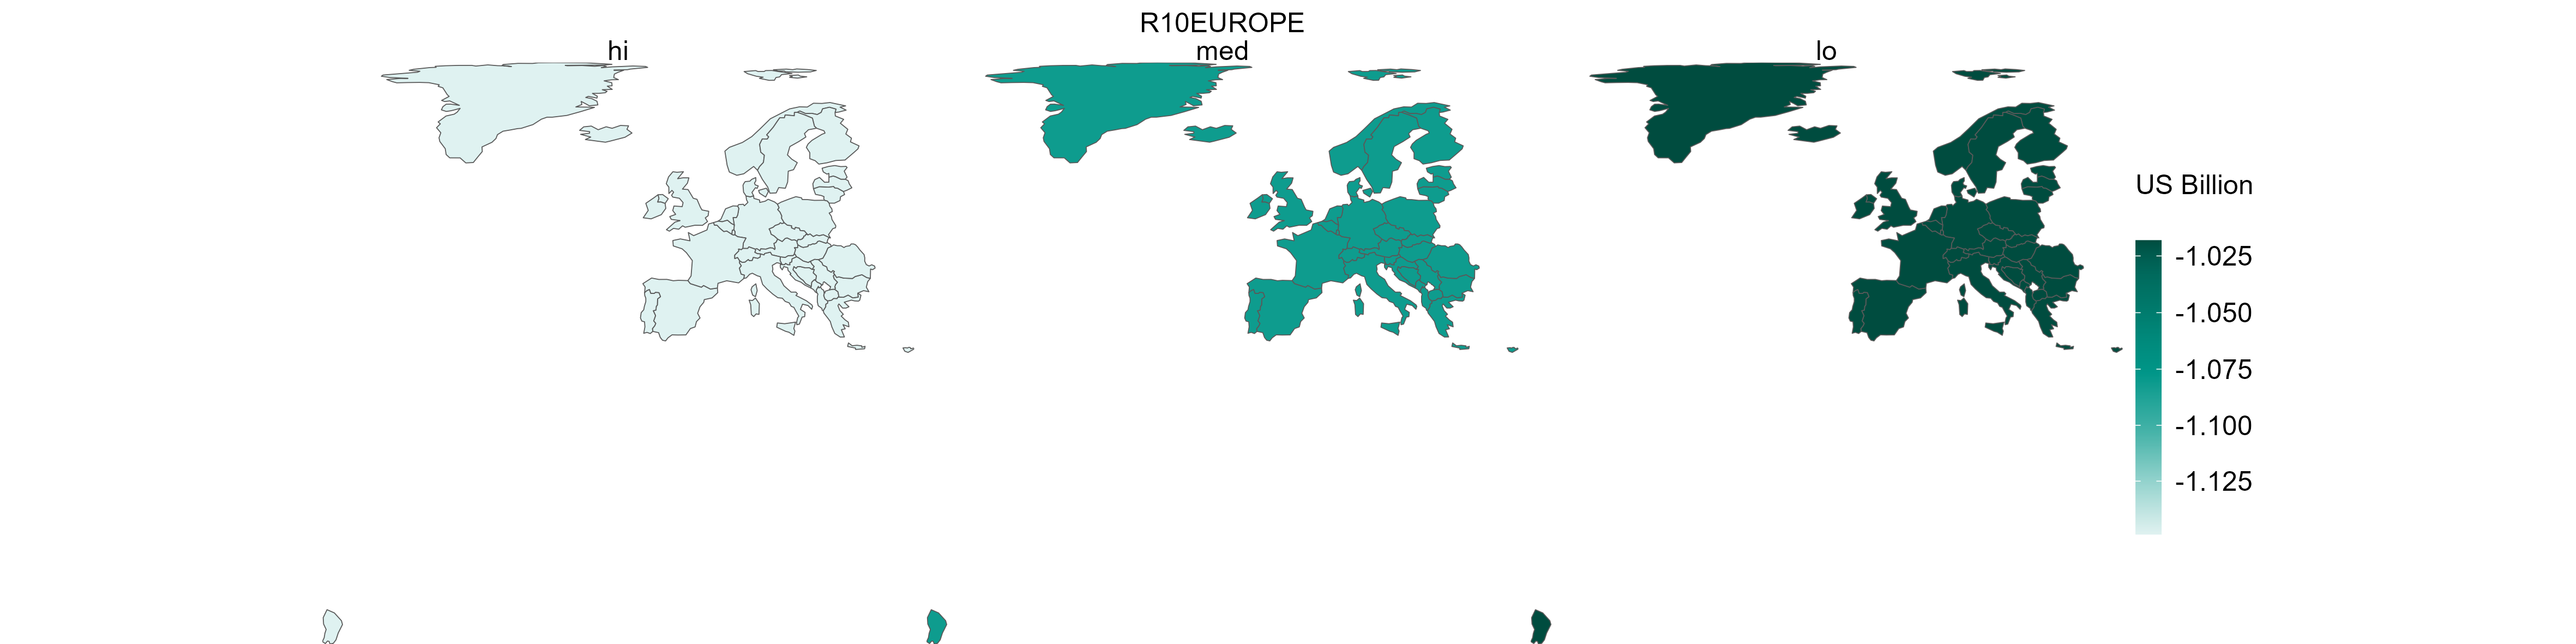
\includegraphics[width=14cm]{"Images_meth/damage_NZ/param_dech/map_param_dech_R10EUROPE.png"}};
    \node[draw=white,rectangle,rounded corners] (india_dech) [below = of northAm_dech, yshift = 1cm] {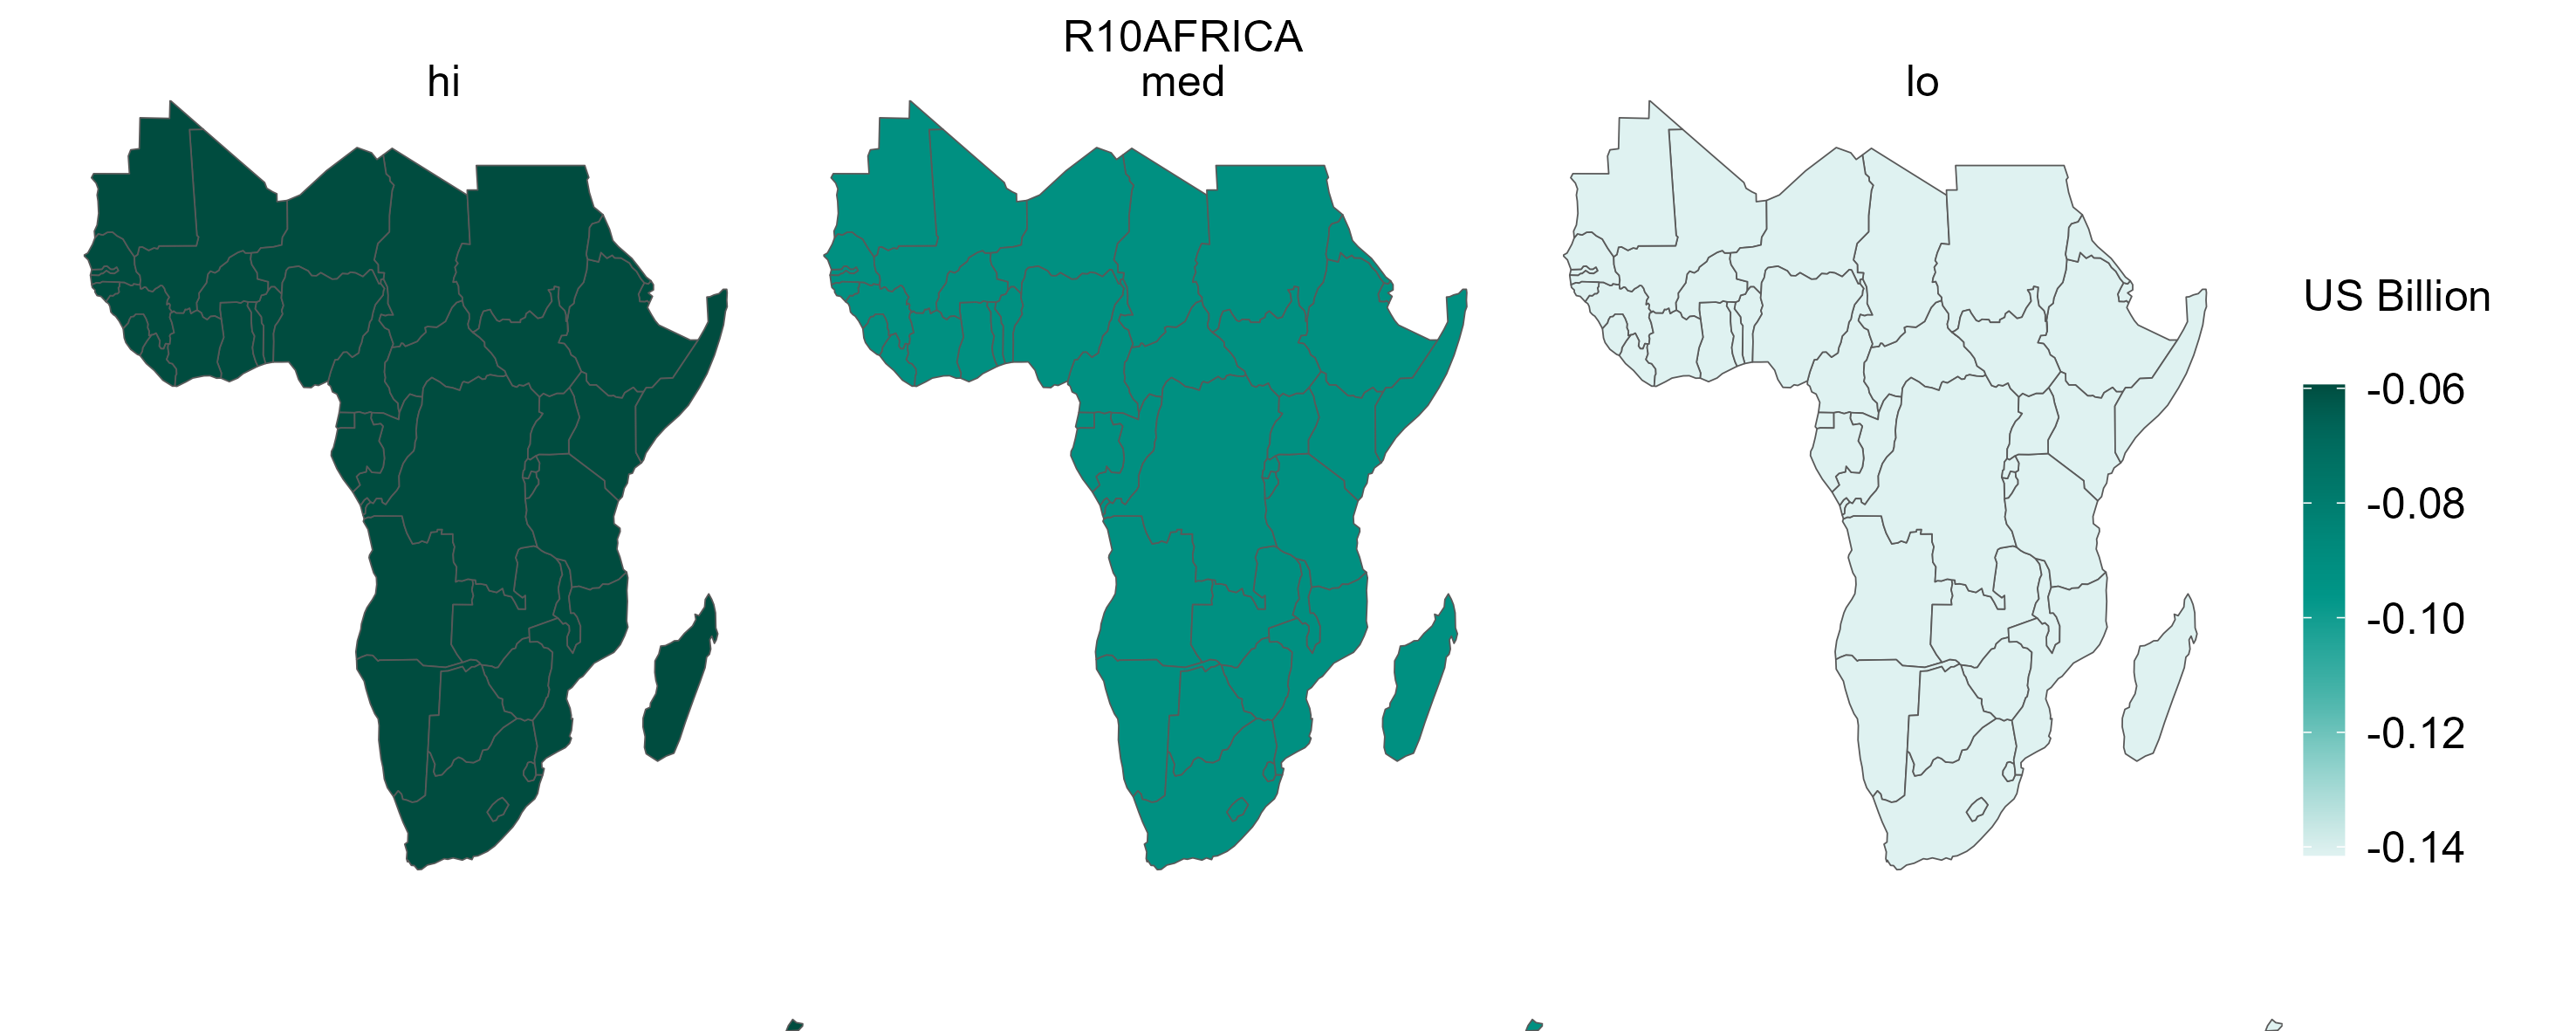
\includegraphics[width=11cm, height=2.75cm, keepaspectratio=FALSE]{"Images_meth/damage_NZ/param_dech/map_param_dech_R10AFRICA.png"}};
    \node[draw=white,rectangle,rounded corners] (a) [above = of northAm_dech, yshift = -1cm]  {\scalebox{0.7}{$\gamma_{i,t} = \gamma_{R10EUROPE, 2015} \cdot \left(\frac{GDPpc_{i,t}}{GDPpc_{R10EUROPE,2015}}\right)^\alpha$}};
  \end{tikzpicture}
  \end{frame}
  
  \begin{frame}{Dechezleprêtre et al. 2019}
    $AvoidedDamage_{i,t,p} = GDP_{i,t,REF} \cdot \gamma_{t,i} \cdot (AP_{i,t,p} - AP_{i,t,REF})$
    \begin{equation*}
      \hspace{10000pt minus 1fil} i \in \{\text{region}\}, t \in \{\text{year}\}, p \in \{\text{policy}\} \hfilneg
    \end{equation*}
  \end{frame}
  
  \begin{frame}{Dechezleprêtre et al. 2019}
    \centering
    \begin{tikzpicture}
      \centering
      \node[draw=white,rectangle,rounded corners] at (-2,0) (northAm_dech) {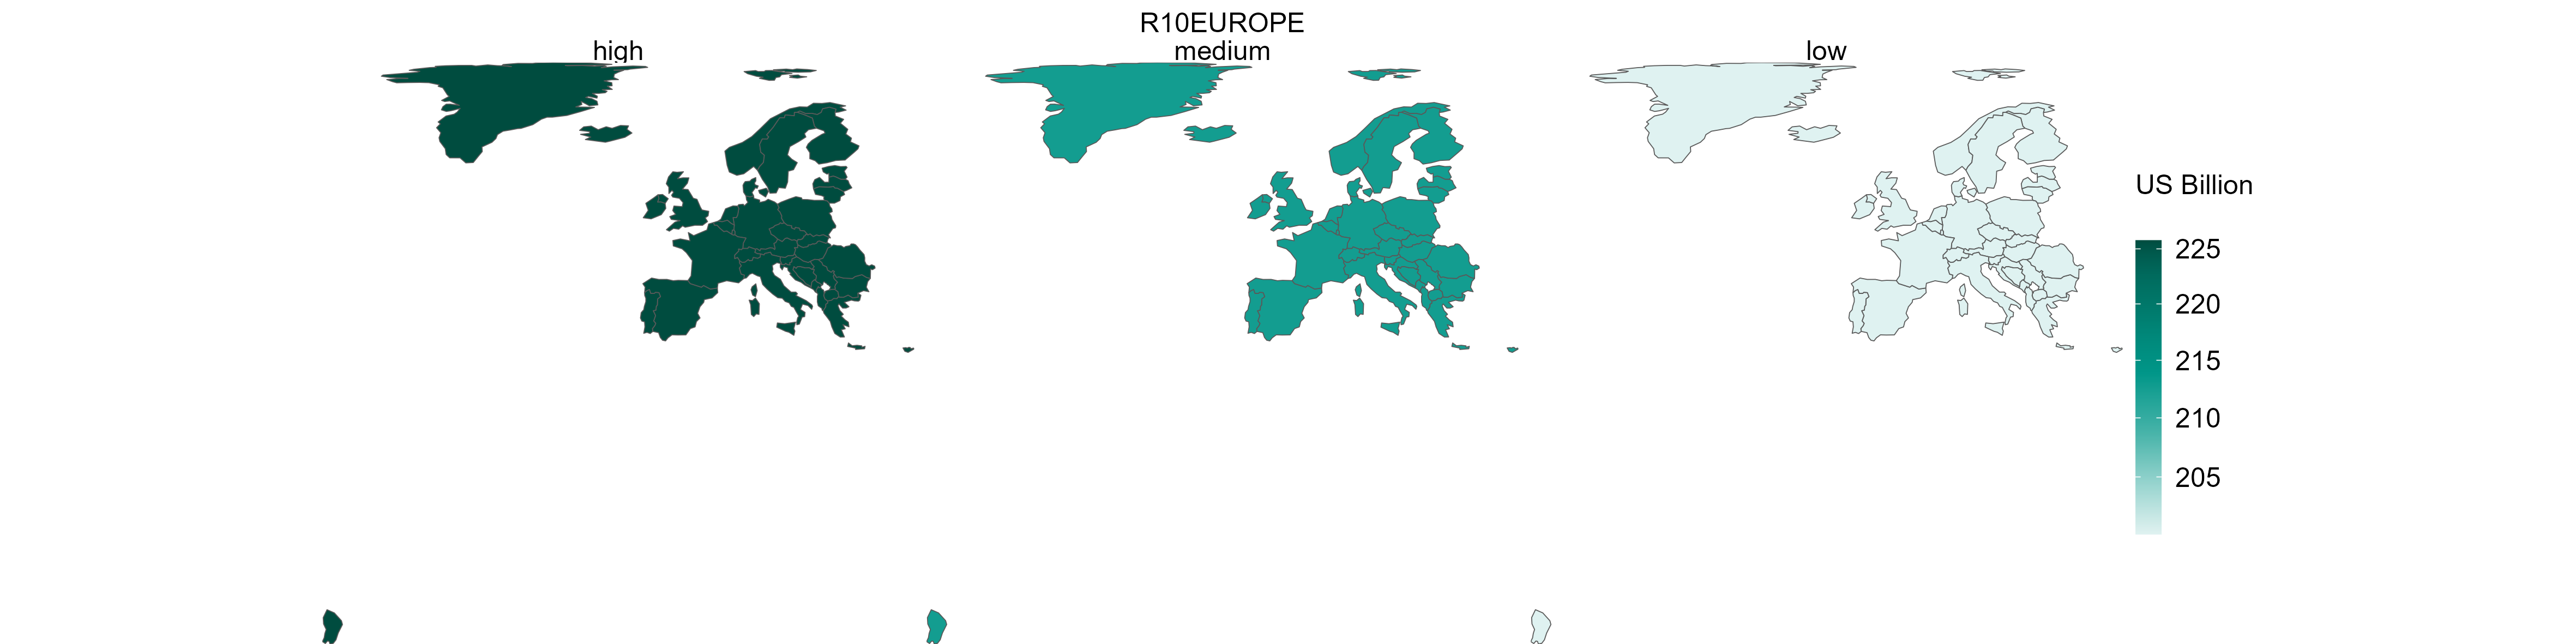
\includegraphics[width=14cm]{"Images_meth/damage_NZ/dech_NZ_median/map_dech_NZ_median_R10EUROPE.png"}};
      \node[draw=white,rectangle,rounded corners] (india_dech) [below = of northAm_dech, yshift = 1cm] {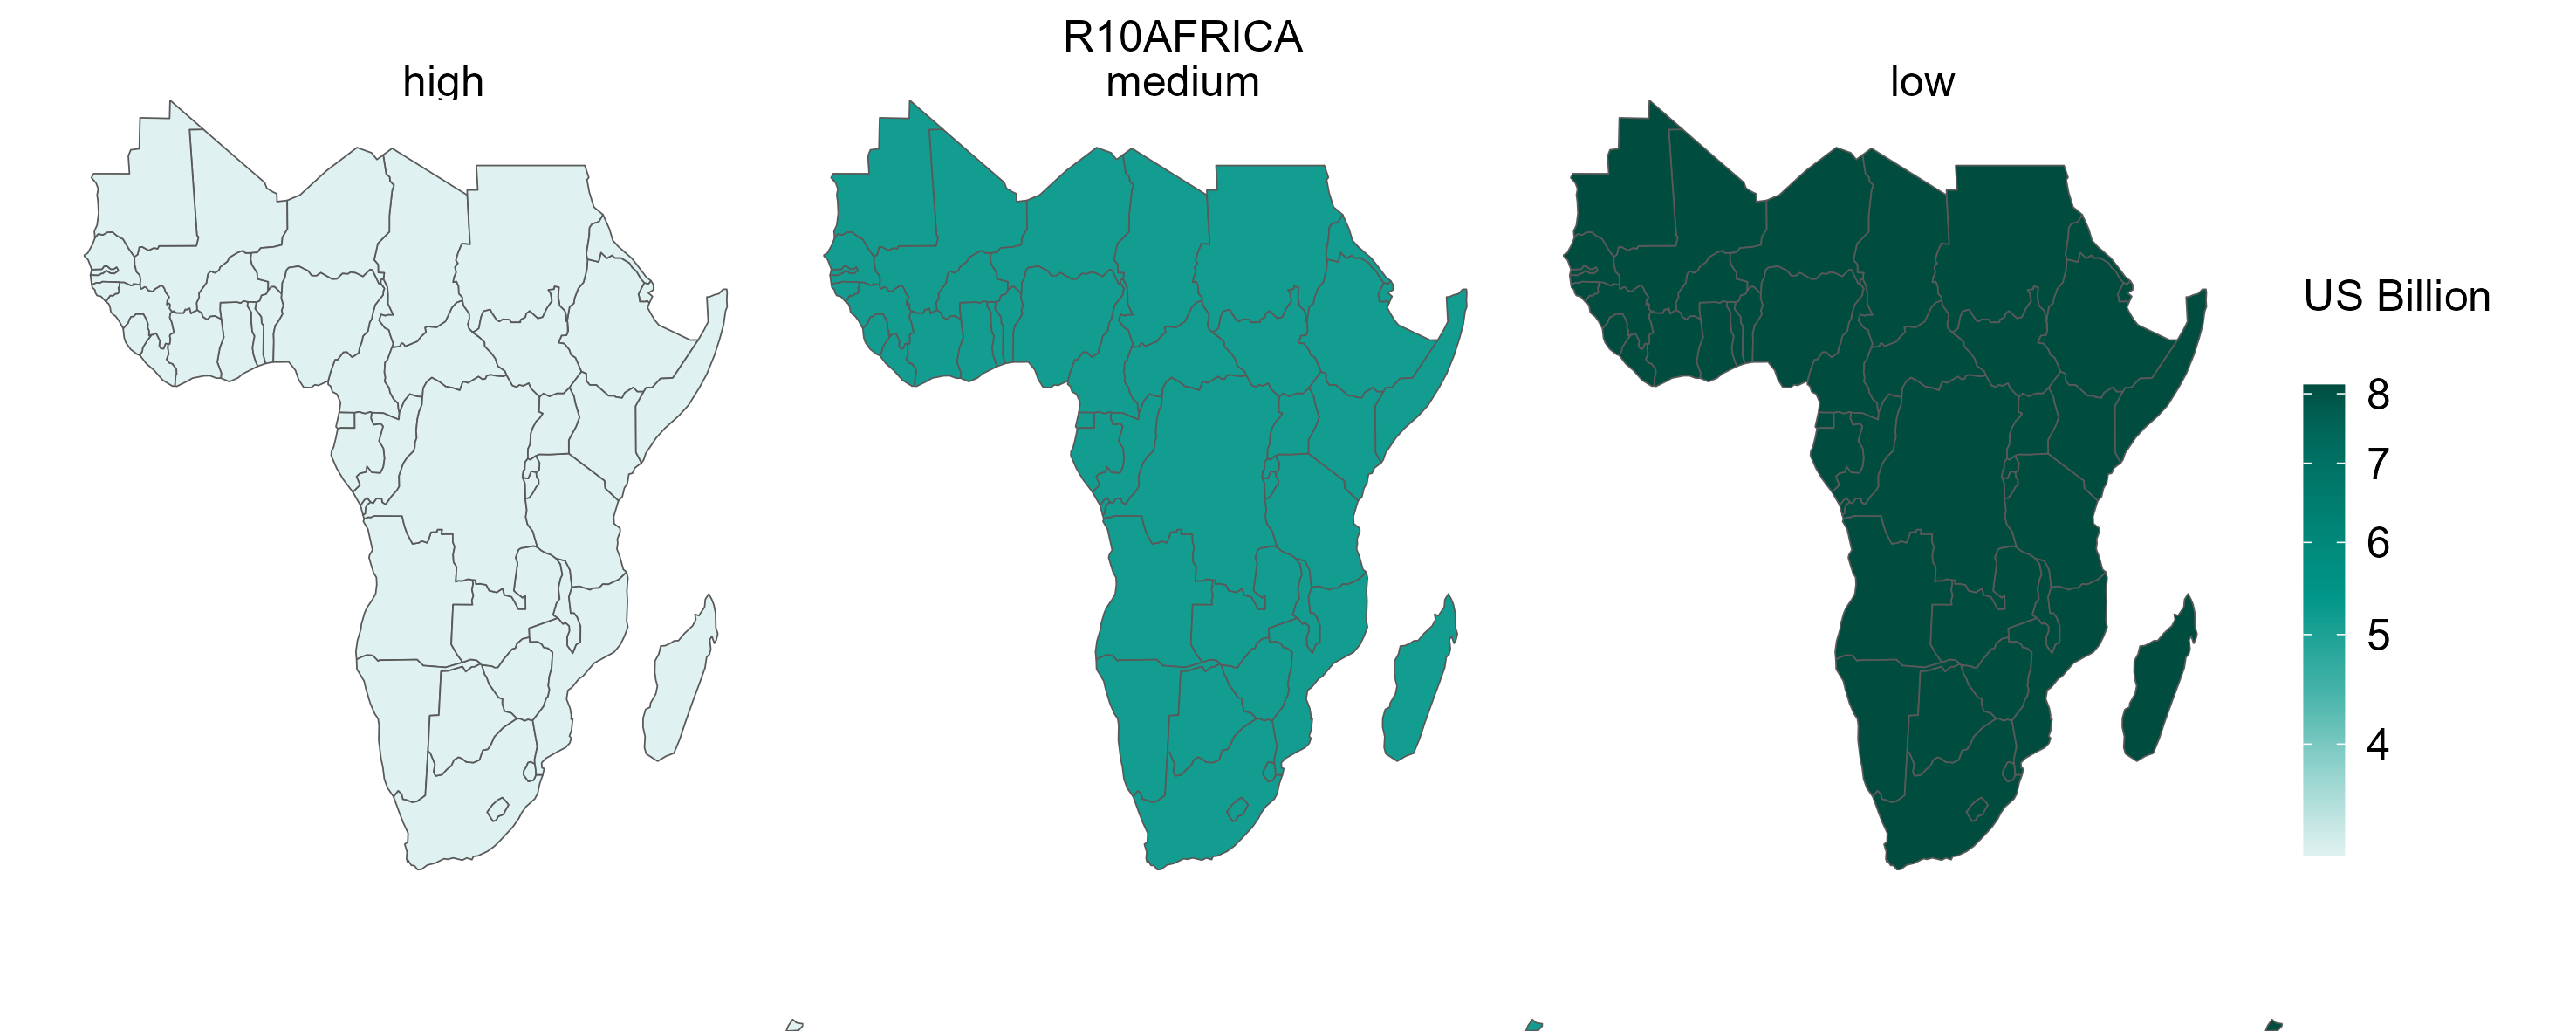
\includegraphics[width=11cm, height=2.75cm, keepaspectratio=FALSE]{"Images_meth/damage_NZ/dech_NZ_median/map_dech_NZ_median_R10AFRICA.png"}};
      \node[draw=white,rectangle,rounded corners] (a) [above = of northAm_dech, yshift = -1cm]  {\scalebox{0.7}{$\Delta ln GDP{i,t} = \gamma_{i,t} \Delta AP_{i,t}, \; \gamma_{i,t} = \gamma_{R10EUROPE, 2015} \cdot \left(\frac{GDPpc_{i,t}}{GDPpc_{R10EUROPE,2015}}\right)^\alpha$}};
    \end{tikzpicture}
    \end{frame}
  
  \begin{frame}{Dechezleprêtre et al. 2019}
    \centering
    \begin{tikzpicture}
      \centering
      \node[draw=white,rectangle,rounded corners] at (0,0) (northAm_dech2) {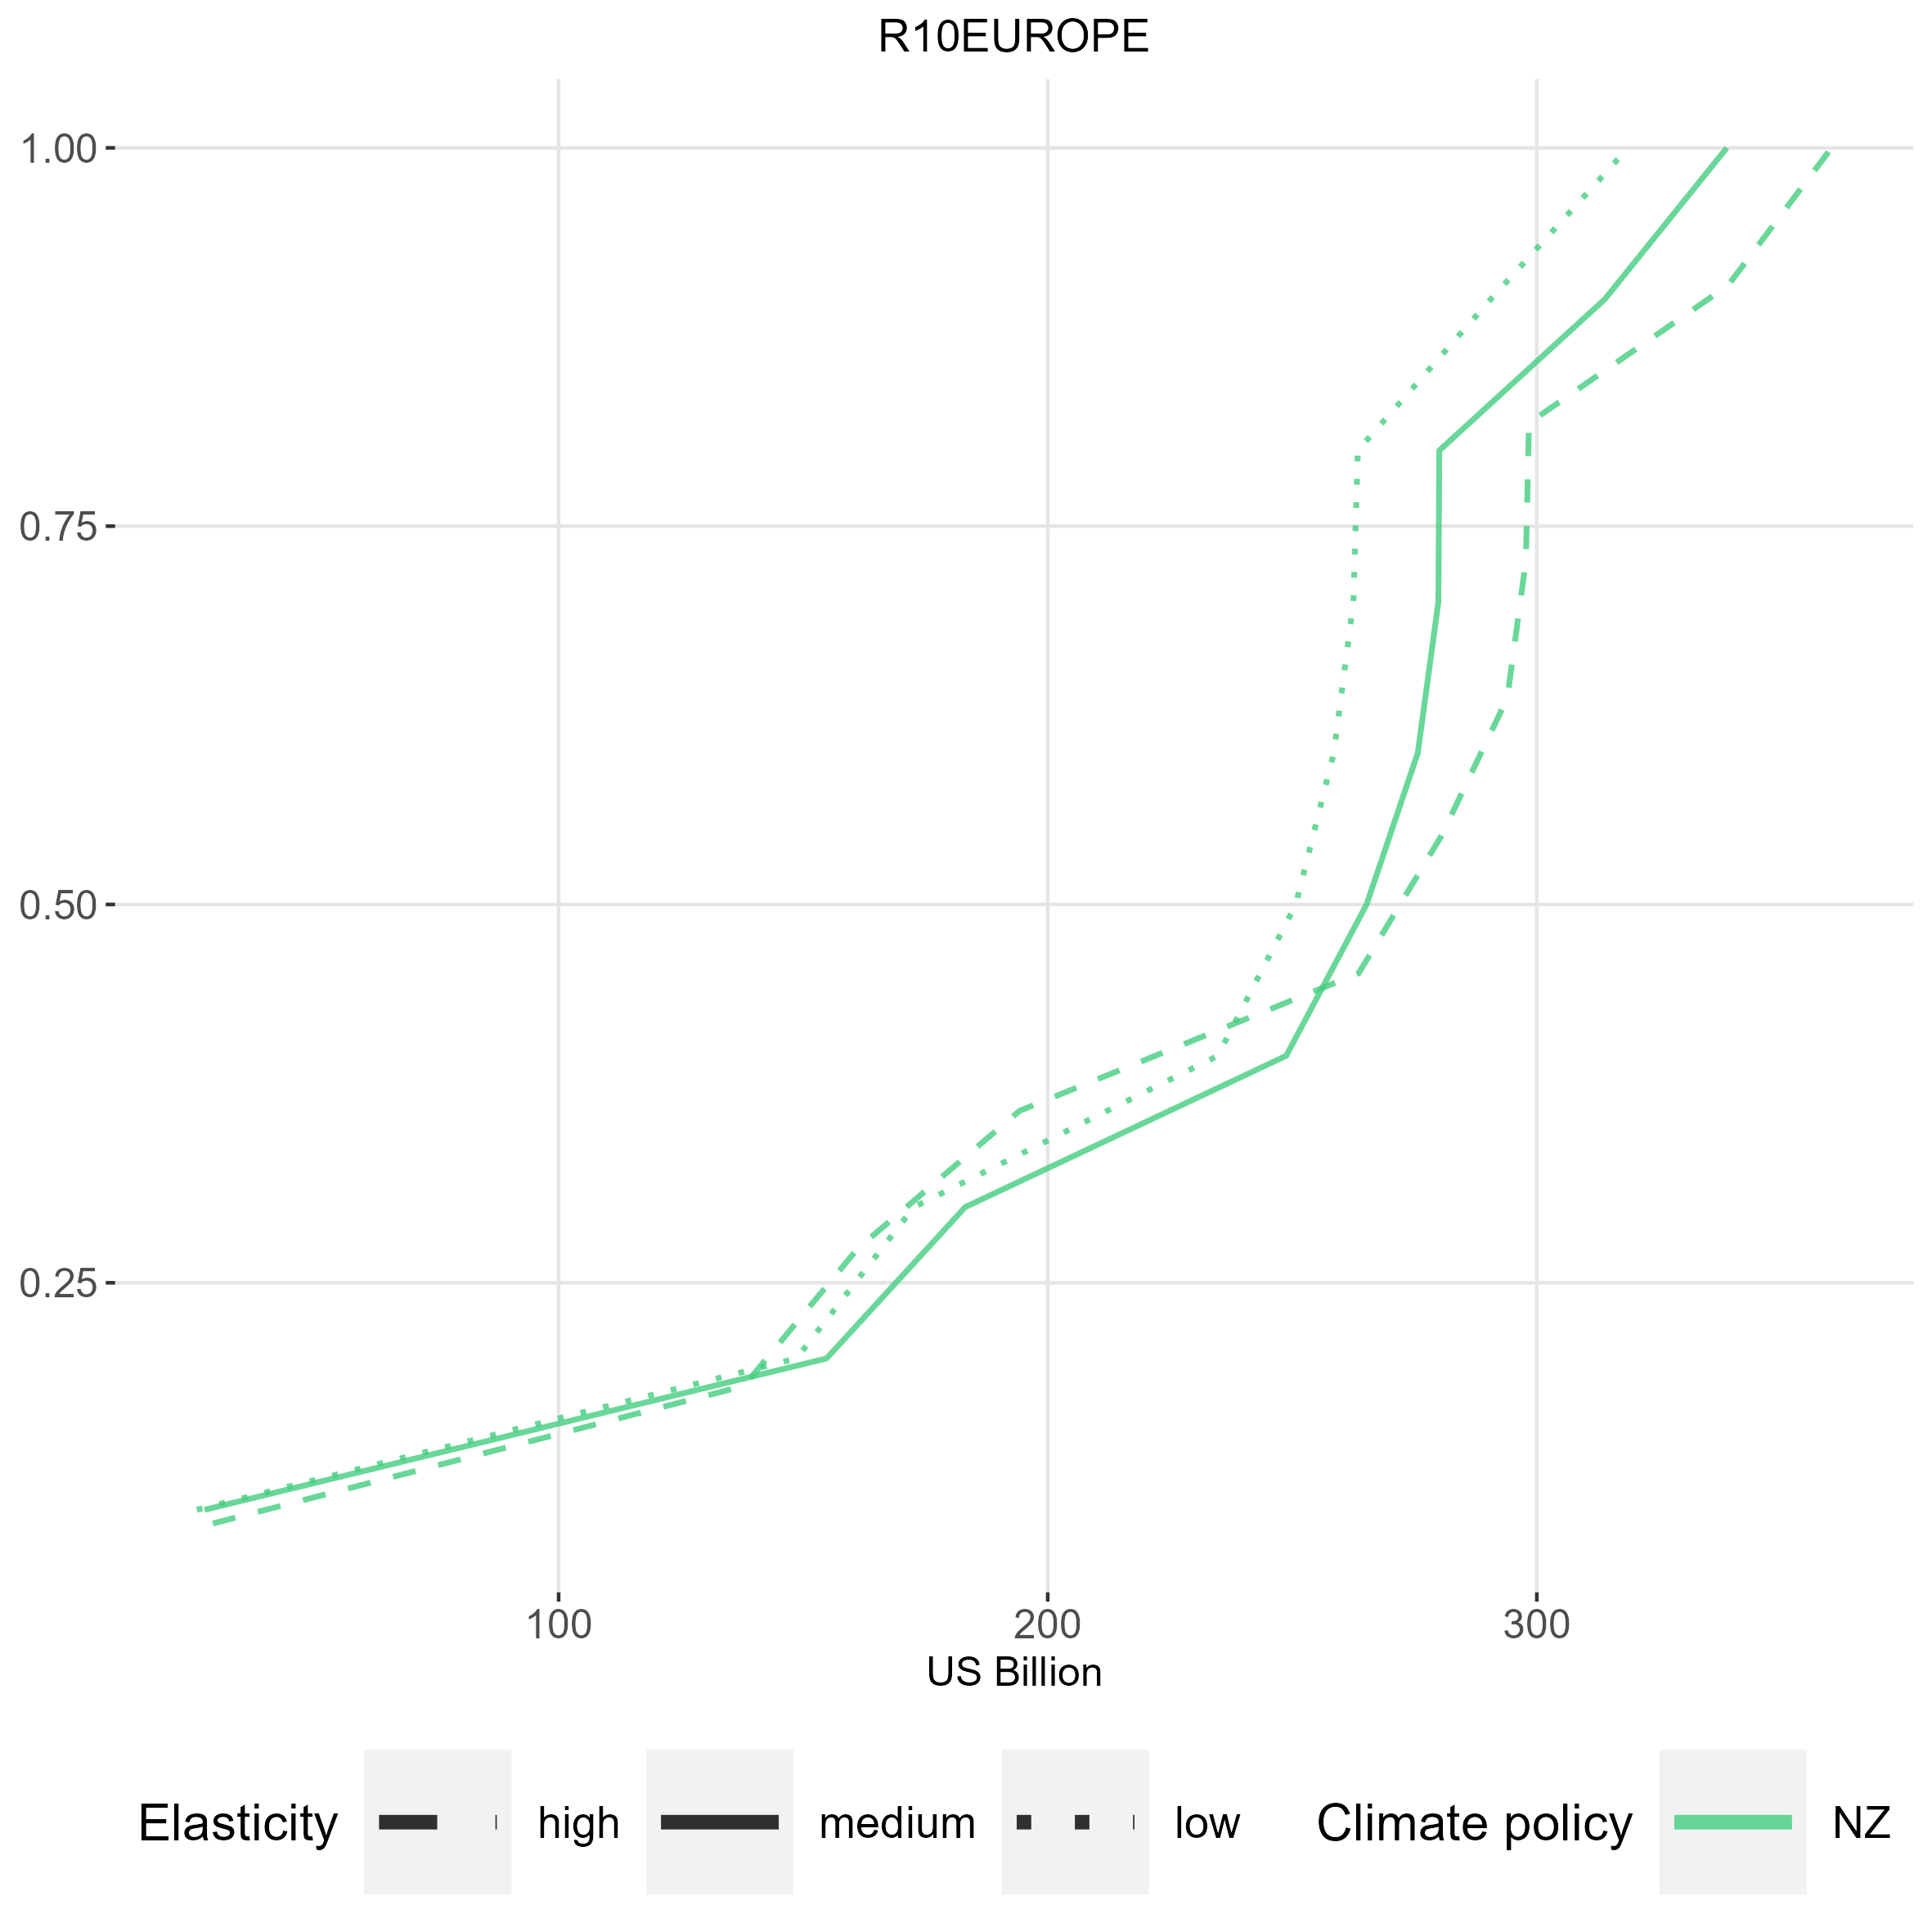
\includegraphics[width=5cm]{"Images_meth/damage_NZ/dech_NZ_median/cum_freq_dech_NZ_median_R10EUROPE.png"}};
      \node[draw=white,rectangle,rounded corners] (india_dech2) [right = of northAm_dech2] {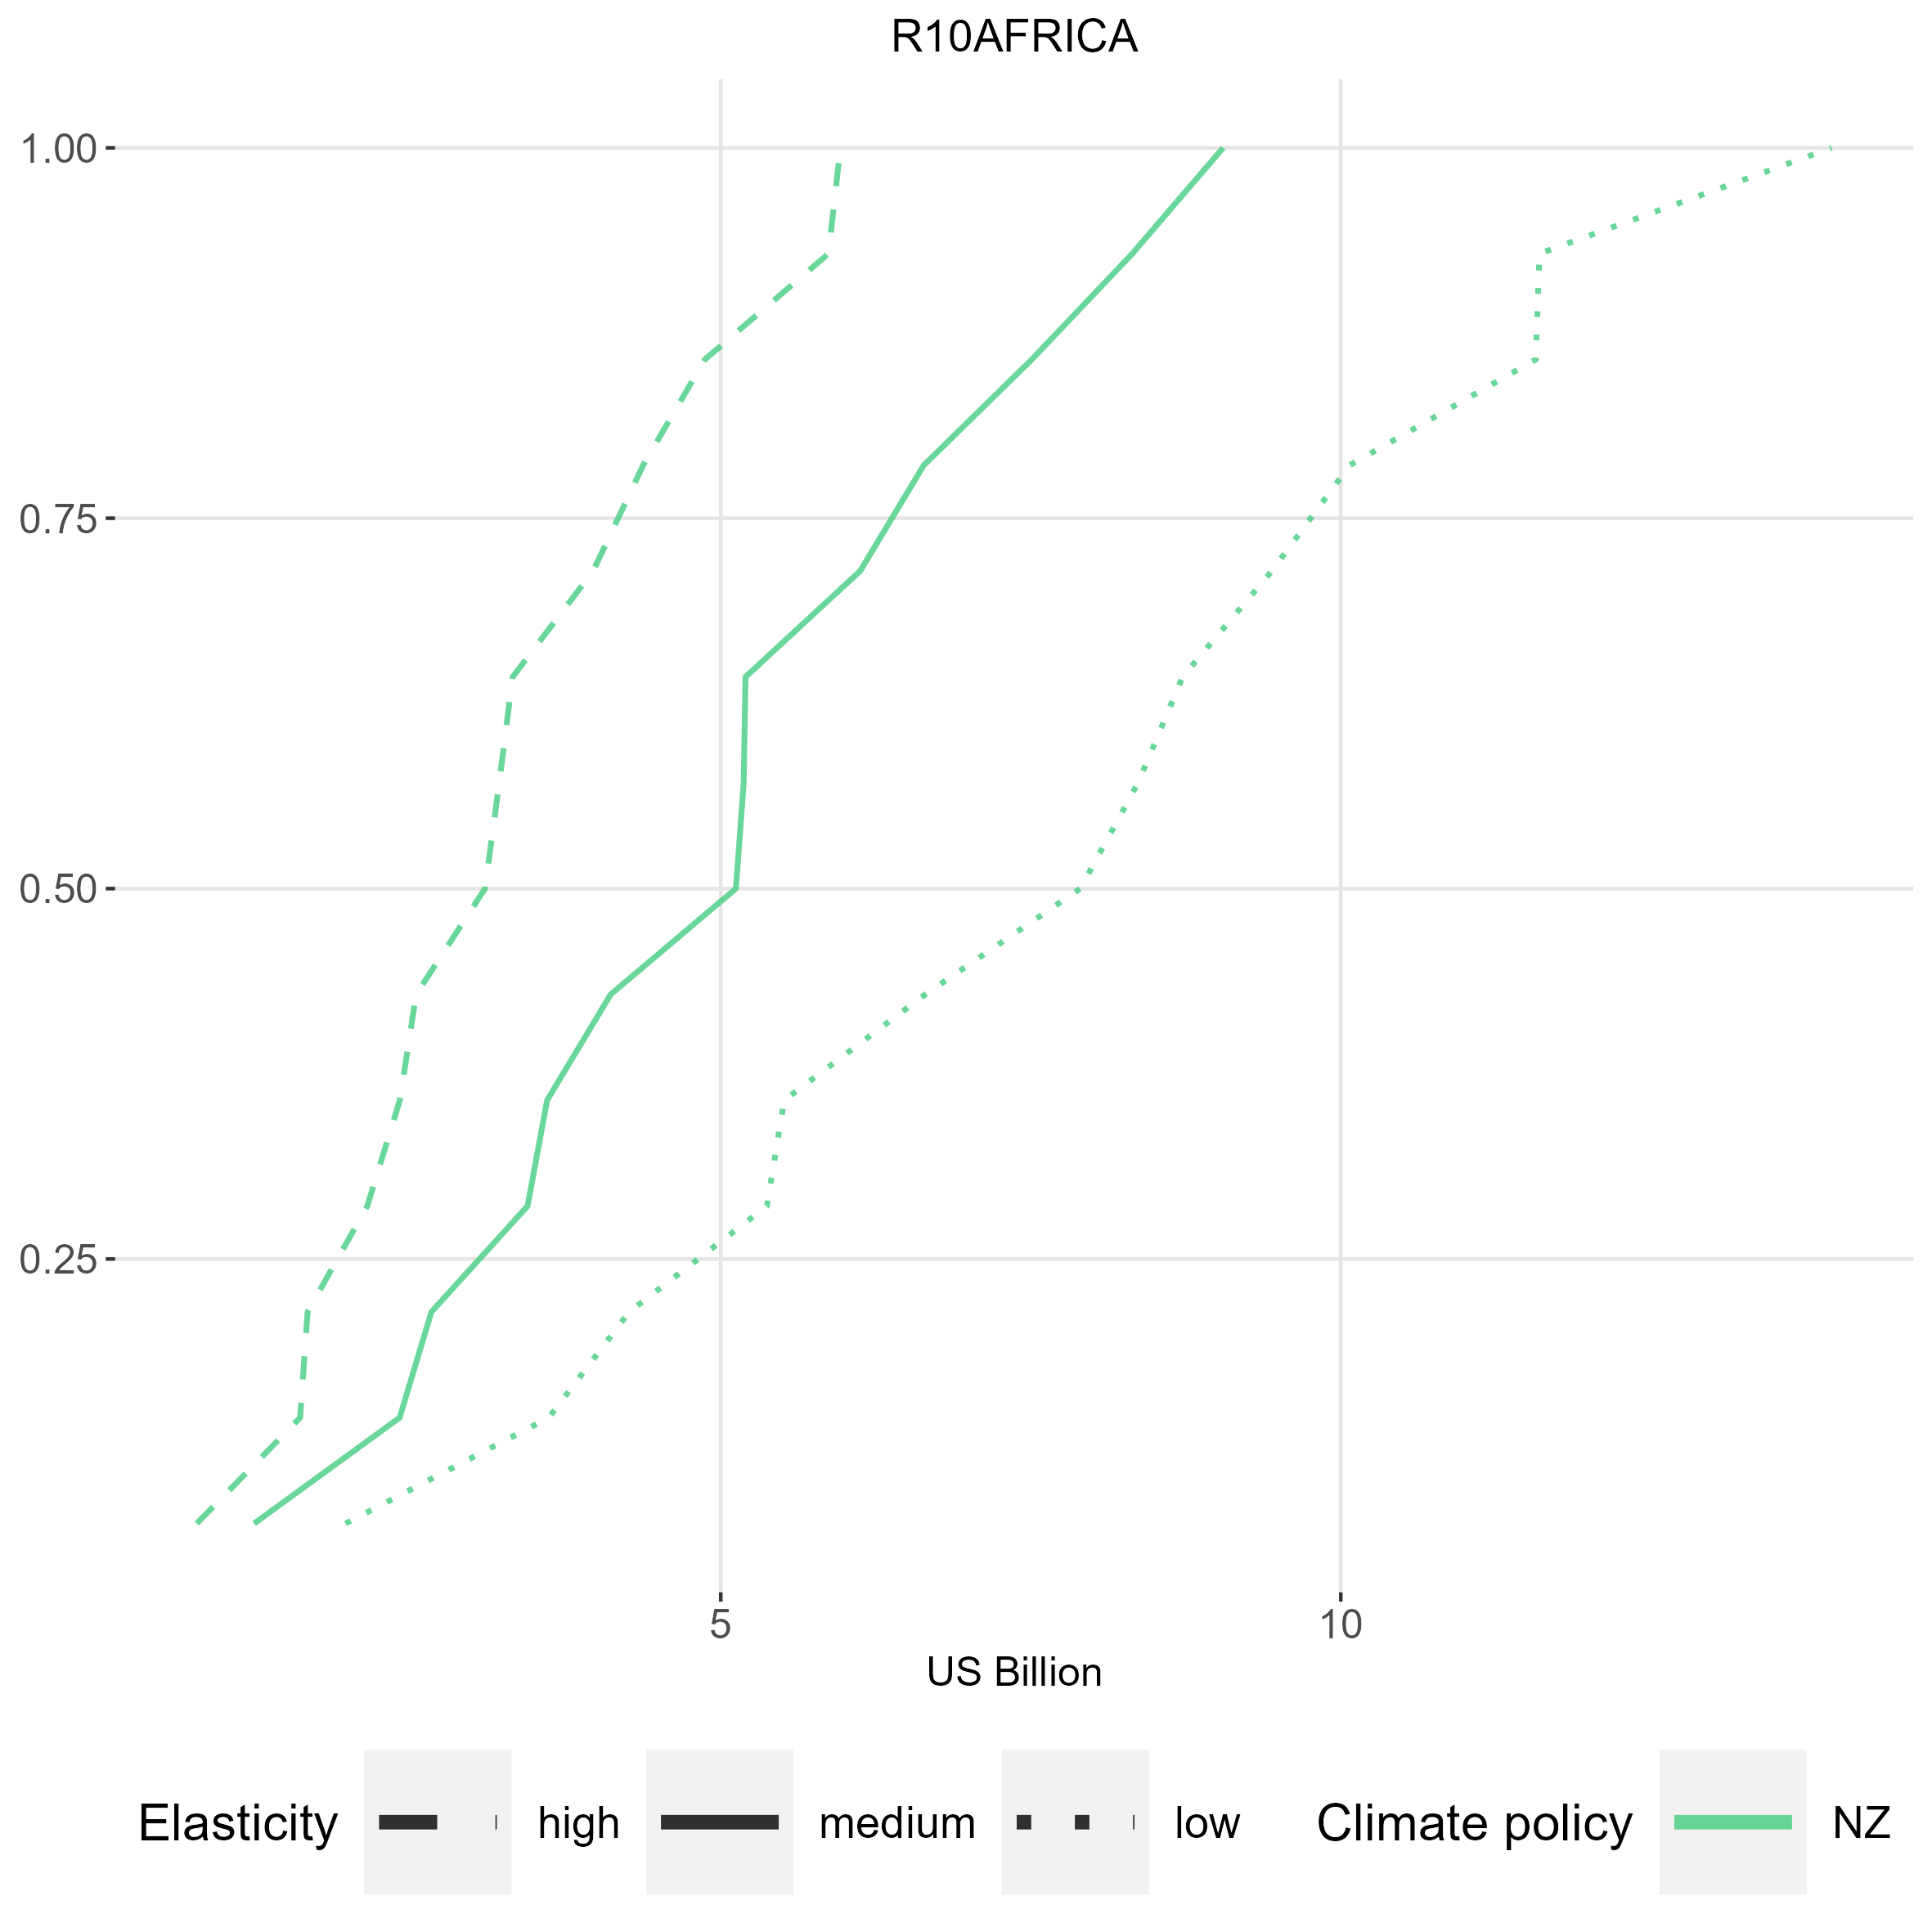
\includegraphics[width=5cm]{"Images_meth/damage_NZ/dech_NZ_median/cum_freq_dech_NZ_median_R10AFRICA.png"}};
      \node[draw=white,rectangle,rounded corners] () [above = of northAm_dech2, xshift = 3cm, yshift = -0.75cm]  {\scalebox{0.7}{$\Delta ln GDP{i,t} = \gamma_{i,t} \Delta AP_{i,t}, \; \gamma_{i,t} = \gamma_{R10EUROPE, 2015} \cdot \left(\frac{GDPpc_{i,t}}{GDPpc_{R10EUROPE,2015}}\right)^\alpha$}};
    \end{tikzpicture}
  \end{frame}

% Dong et al. 2021 %------------------------------------------------%------------------------------------------------%------------------------------------------------

\begin{frame}{Dong et al. 2021}
% In 2021, Dong et al. [11] developed another econometric model, this time, based on China. The aim of the model is to estimate the economic growth considering air pollution and other factors. 
% Like in Dechezleprêtre’s model, we only account for the air pollution factor since we aim to see the impact of this item solely. Thus, the GDP growth equation for region i, year t, and policy p is
$$\tikzmark{GDPini} GDPgrowth_{i,t} = \beta_{1} \tikzmark{AP} AP_{i,t} + \beta_2 \tikzmark{province} s_i + \beta_3 \tikzmark{time} \nu_t + \tikzmark{error} \varepsilon_{i,t}$$
\vspace{0.5cm}
\only<1-2>{
    \begin{equation*}
        \hspace{10000pt minus 1fil} i \in \{\text{region}\} \hfilneg
    \end{equation*}
    \begin{equation*}
        \hspace{10000pt minus 1fil} t \in \{\text{year}\} \hfilneg
    \end{equation*}
}
\onslide<3-6>{
    \begin{equation*}
        \hspace{10000pt minus 1fil} i \in \text{ region,} \; t \in \{\text{year}\} \hfilneg
    \end{equation*}
}

\onslide<3-6>{$$\tikzmark{GDPsimplified} GDPgrowthNEW_{i,t} = GDPgrowthBASE_{i,t} + \tikzmark{bb}\beta_{i,t} AP_{i,t}$$ }

\only<5-6>{$$\beta_{i,t} = \beta_{R10CHINA, 2015} \cdot \left(\frac{GDPpc_{i,t}}{GDPpc_{R10CHINA,2015}}\right)^\alpha\tikzmark{elasticity}, \; \; \alpha \in \{0.8, 1, 1.2\}$$ }

\begin{tikzpicture}[remember picture,overlay]
\onslide<2-6>{
% air pollution
\draw[<-] 
  ([shift={(7pt,15pt)}]pic cs:AP) |- ([shift={(17pt,23pt)}]pic cs:AP) 
  node[anchor=west] {$\scriptstyle \text{\pmm}$}; 
\draw[] 
  ([shift={(7pt,15pt)}]pic cs:AP)  ([shift={(17pt,15pt)}]pic cs:AP) 
  node[anchor=west] {$\scriptstyle \text{concentration}$};
% province effects
\draw[<-] 
  ([shift={(3pt,-8pt)}]pic cs:province) |- ([shift={(13pt,-16pt)}]pic cs:province) 
  node[anchor=west] {$\scriptstyle \text{fixed}$}; 
\draw[] 
  ([shift={(3pt,-8pt)}]pic cs:province)  ([shift={(13pt,-24pt)}]pic cs:province) 
  node[anchor=west] {$\scriptstyle \text{regional effects}$}; 
% time effects
\draw[<-] 
  ([shift={(5pt,15pt)}]pic cs:time) |- ([shift={(15pt,23pt)}]pic cs:time) 
  node[anchor=west] {$\scriptstyle \text{fixed time effects}$}; 
% error
\draw[<-] 
  ([shift={(3pt,-8pt)}]pic cs:error) |- ([shift={(15pt,-16pt)}]pic cs:error) 
  node[anchor=west] {$\scriptstyle \text{random disturbance}$}; 
\draw[] 
  ([shift={(3pt,-8pt)}]pic cs:error)  ([shift={(15pt,-24pt)}]pic cs:error) 
  node[anchor=west] {$\scriptstyle \text{term}$}; 
}
% arrow
\onslide<3-6>{\draw [->,black] (pic cs:GDPini) to [out=200,in=-150] node {} (pic cs:GDPsimplified);}
% circle around gamma
\onslide<4-6>{\draw[red] ([xshift=7pt, yshift=2pt]pic cs:bb) circle [radius=10pt];}
% elasticity
\only<6>{\draw[<-] 
  ([shift={(-4.5pt,20pt)}]pic cs:elasticity) |- ([shift={(5pt,28pt)}]pic cs:elasticity) 
  node[anchor=west] {$\scriptstyle \text{elasticity}$}; }
\end{tikzpicture}
\vfill \hfill \cite{dong_adverse_2021}
\end{frame}

\begin{frame}{Dong et al. 2021}
  \centering
  \begin{table}[]
    \begin{tabular}{llll}
    \textbf{region}    & \textbf{year} & \begin{tabular}[c]{@{}l@{}}\textbf{GDP}\\ \textbf{{[}billion US$\$$2010/yr{]}}\end{tabular} & \begin{tabular}[c]{@{}l@{}}\textbf{population}\\ \textbf{{[}nº people{]}}\end{tabular} \\ \hline
    R10AFRICA          & 2030          & 6690.474                                                                                  & 1690667000                                                                             \\
    R10CHINA+          & 2030          & 38588.497                                                                                 & 1416996000                                                                             \\
    R10EUROPE          & 2030          & 21838.421                                                                                 & 500700000                                                                              \\
    R10INDIA+          & 2030          & 14680.280                                                                                 & 1593797000                                                                             \\
    R10LATIN\_AM       & 2030          & 13126.332                                                                                 & 693664000                                                                              \\
    R10MIDDLE\_EAST NZ & 2030          & 9314.170                                                                                  & 576311000                                                                              \\
    R10NORTH\_AM       & 2030          & 24351.917                                                                                 & 424540000                                                                              \\
    R10PAC\_OECD       & 2030          & 7567.581                                                                                  & 210367000                                                                              \\
    R10REF\_ECON       & 2030          & 6518.265                                                                                  & 320831000                                                                              \\
    R10REST\_ASIA      & 2030          & 13674.476                                                                                 & 1411653000                                                                              \\
    R10CHINA           & 2015          & 18548.173                                                                                 & 1433079780                                                          
    \end{tabular}
    \end{table}
    $\beta_{R10CHINA,2015} = -0.02108$
\end{frame}

\begin{frame}{Dong et al. 2021}
  \centering
  \begin{tikzpicture}
    \centering
    \node[draw=white,rectangle,rounded corners] at (0,0) (northAm_dong) {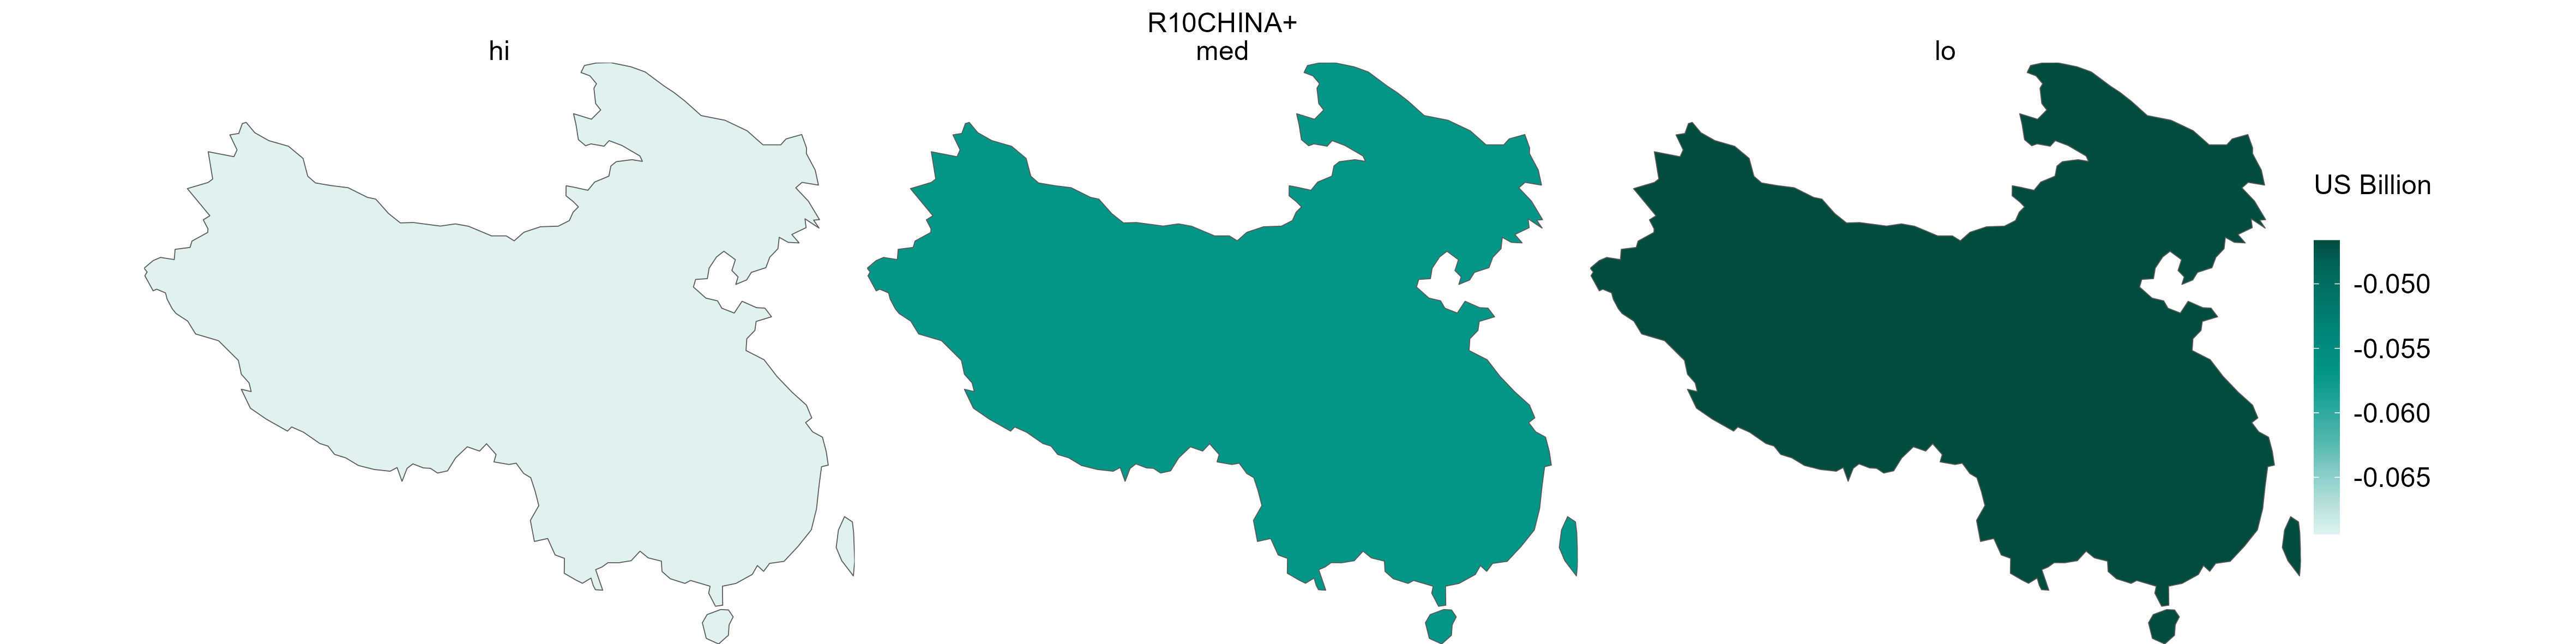
\includegraphics[width=11cm]{"Images_meth/damage_NZ/param_dong/map_param_dong_R10CHINA+.png"}};
    \node[draw=white,rectangle,rounded corners] (india_dong) [below = of northAm_dong, yshift = 0.75cm] {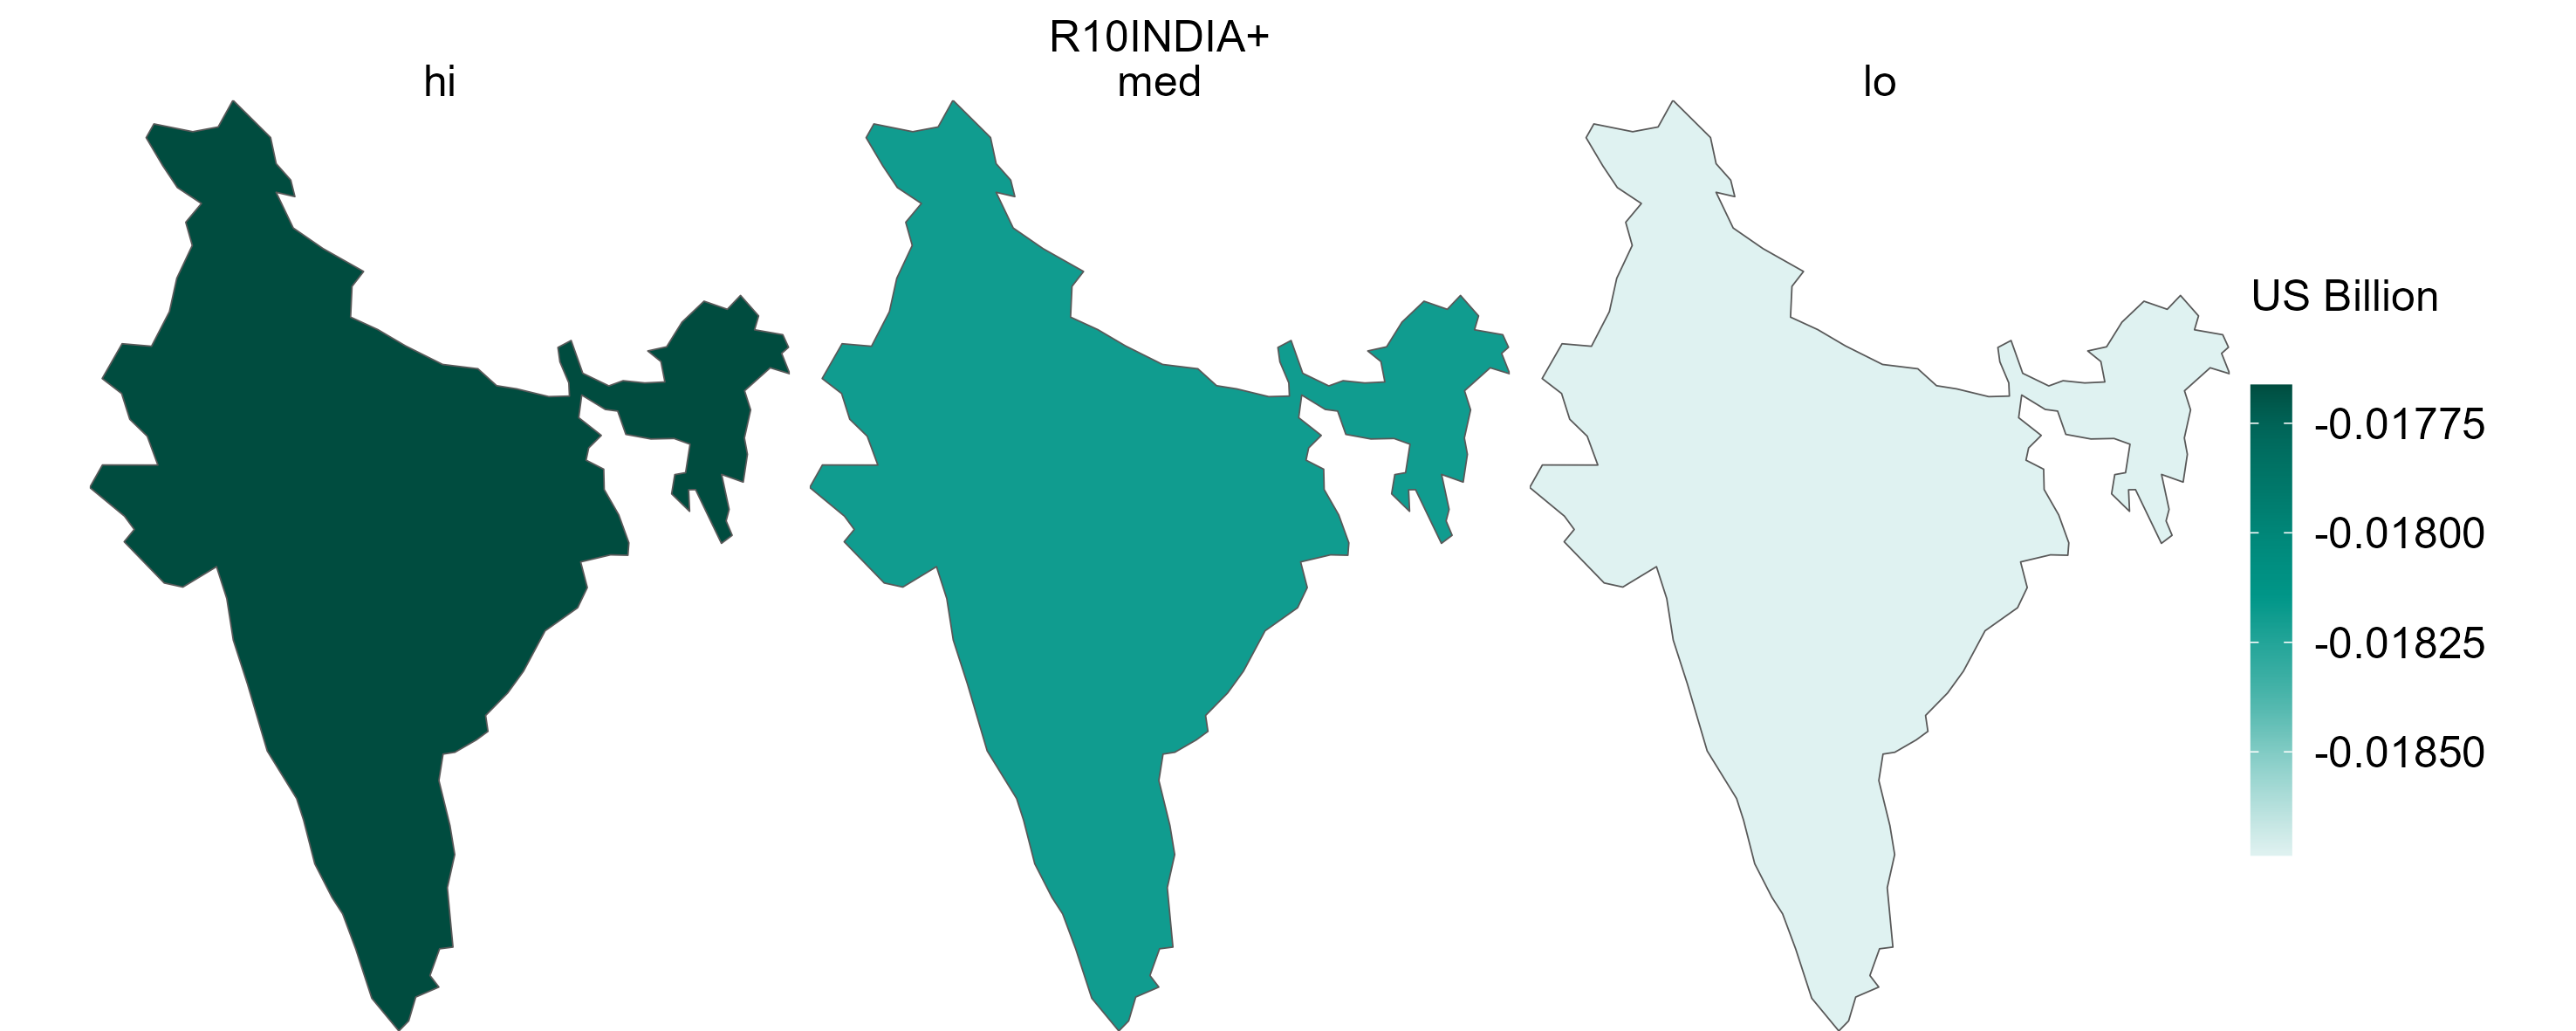
\includegraphics[width=11cm, height=3cm, keepaspectratio=FALSE]{"Images_meth/damage_NZ/param_dong/map_param_dong_R10INDIA+.png"}};
    \node[draw=white,rectangle,rounded corners] (aa) [above = of northAm_dong, yshift = -1cm]  {\scalebox{0.6}{$\beta_{i,t} = \beta_{R10CHINA, 2015} \cdot \left(\frac{GDPpc_{i,t}}{GDPpc_{R10CHINA,2015}}\right)^\alpha$}};
  \end{tikzpicture}
  \end{frame}
  

\begin{frame}{Dong et al. 2021}
  $$GDPnew_{i,t} = GDPbase_{i,t} \cdot (1 + GDPgrowthNEW_{i,t})$$
  \vspace{1cm}
  $AvoidedDamage_{i,t,p} = GDPnew_{i,t,p} - GDPnew_{i,t,REF}$
  \begin{equation*}
    \hspace{10000pt minus 1fil} i \in \{\text{region}\}, t \in \{\text{year}\}, p \in \{\text{policy}\} \hfilneg
  \end{equation*}
\end{frame}


\begin{frame}{Dong et al. 2021}
  \centering
  \begin{tikzpicture}
    \centering
    \node[draw=white,rectangle,rounded corners] at (0,0) (northAm_dong) {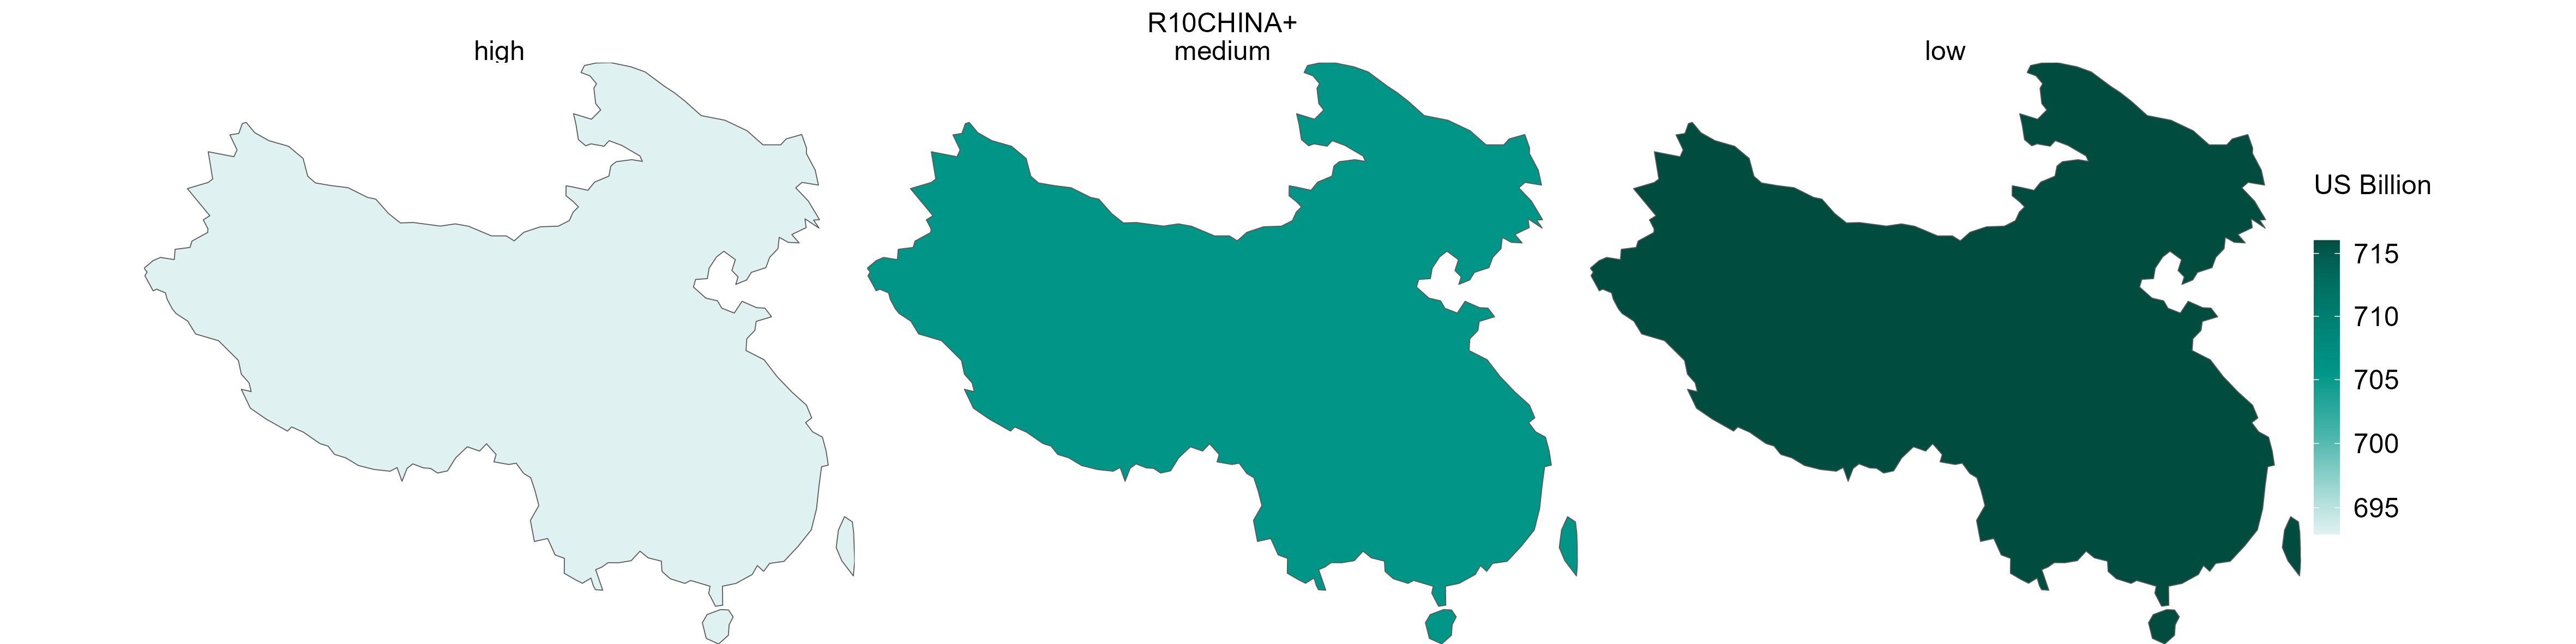
\includegraphics[width=11cm]{"Images_meth/damage_NZ/dong_NZ_median/map_dong_NZ_median_R10CHINA+.png"}};
    \node[draw=white,rectangle,rounded corners] (india_dong) [below = of northAm_dong, yshift = 0.75cm] {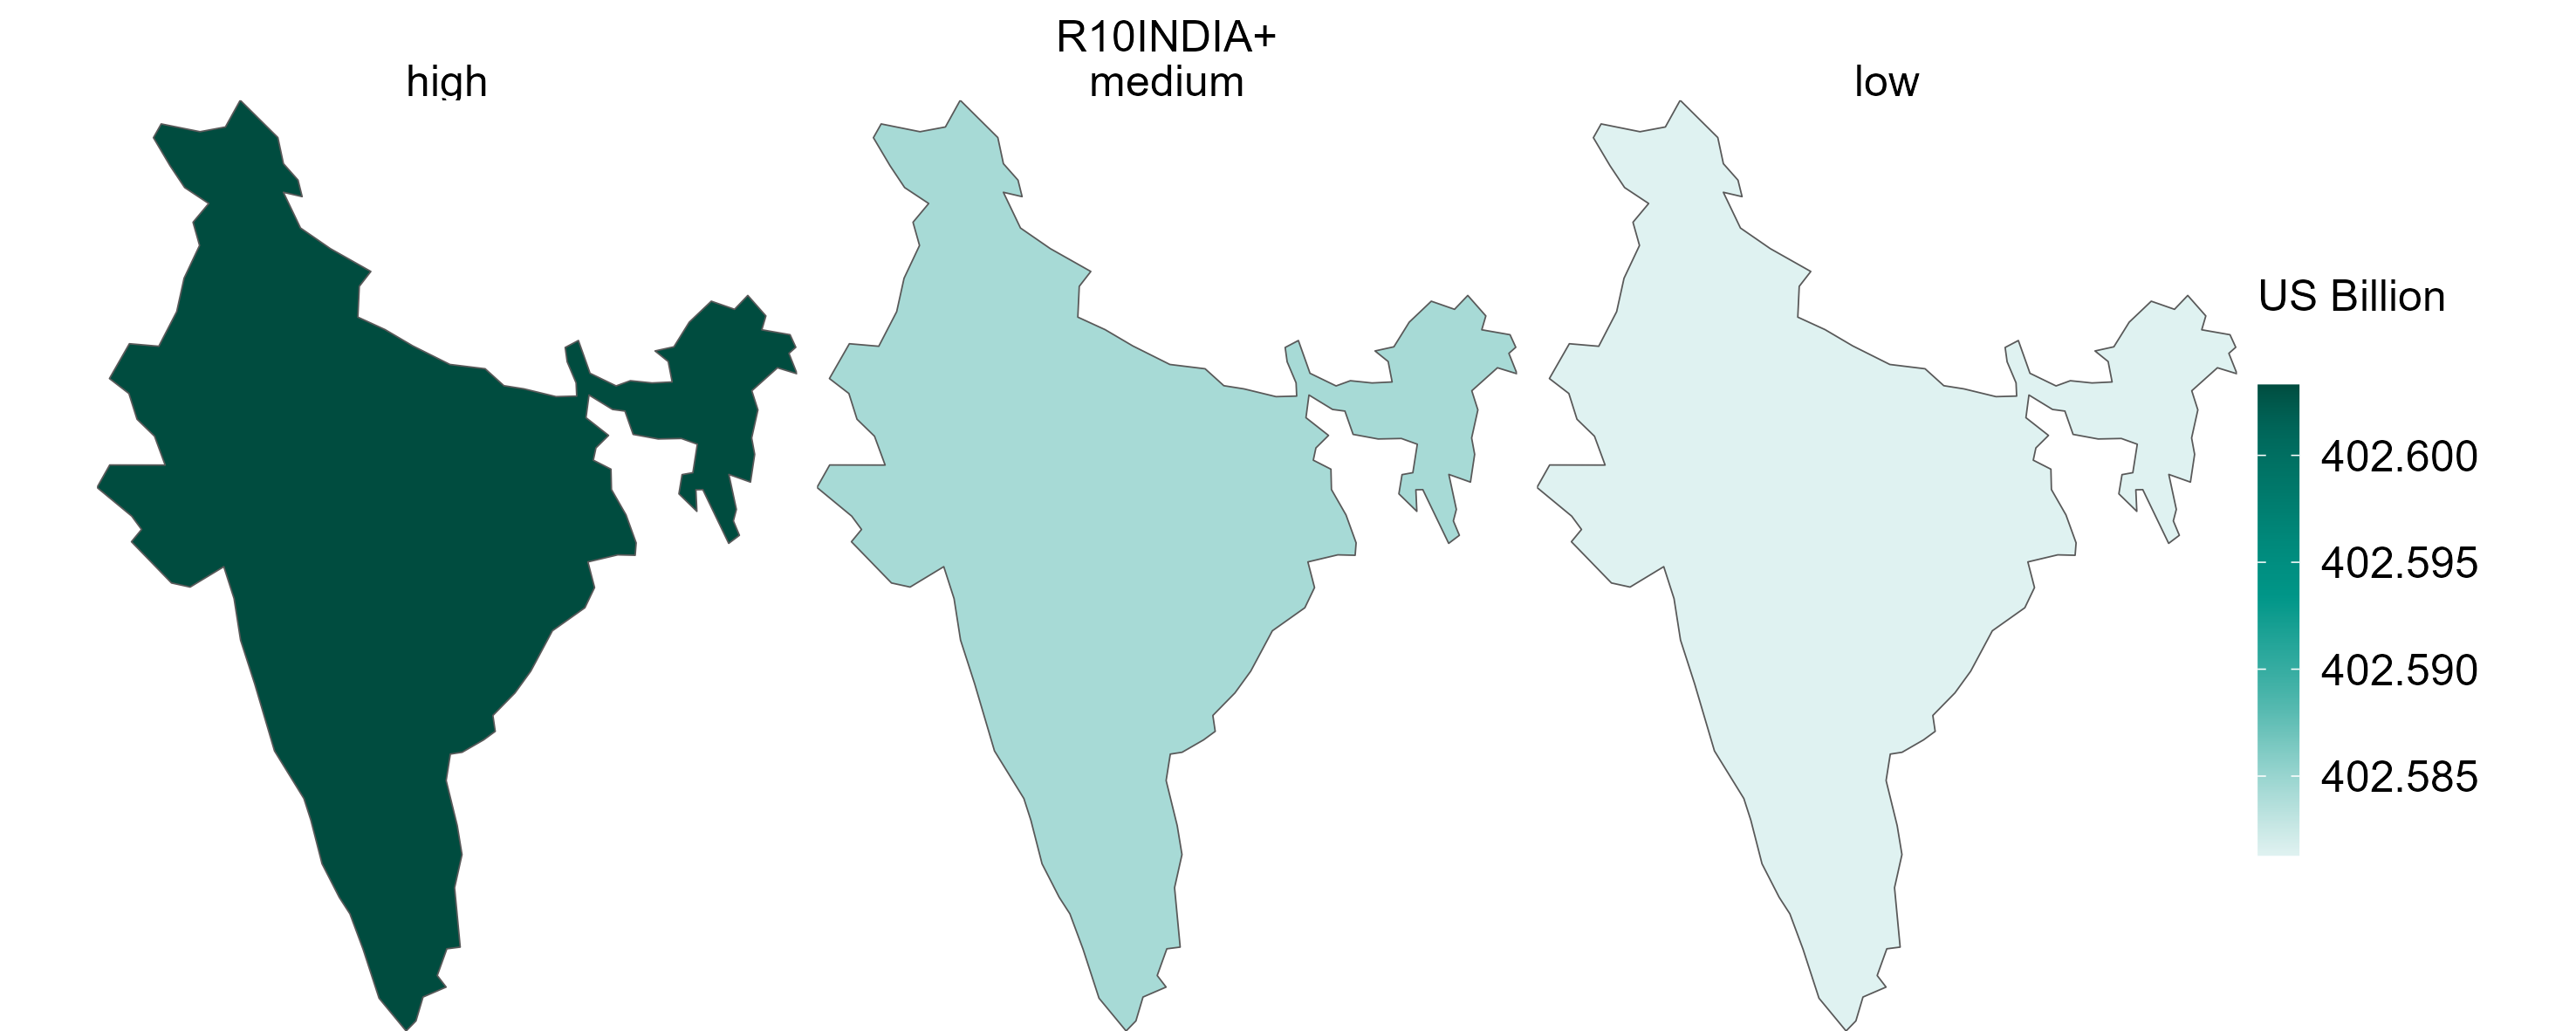
\includegraphics[width=11cm, height=3cm, keepaspectratio=FALSE]{"Images_meth/damage_NZ/dong_NZ_median/map_dong_NZ_median_R10INDIA+.png"}};
    \node[draw=white,rectangle,rounded corners] (aa) [above = of northAm_dong, yshift = -0.5cm]  {\scalebox{0.6}{$AvoidedDamage_{i,t,p} = GDPnew_{i,t,p} - GDPnew_{i,t,REF}$}};
    \node[draw=white,rectangle,rounded corners] (aa) [above = of northAm_dong, yshift = -1cm]  {\scalebox{0.6}{$GDPgrowthNEW_{i,t} = GDPgrowthBASE_{i,t} + \beta_{i,t} AP_{i,t}, \; \beta_{i,t} = \beta_{R10CHINA, 2015} \cdot \left(\frac{GDPpc_{i,t}}{GDPpc_{R10CHINA,2015}}\right)^\alpha$}};
  \end{tikzpicture}
  \end{frame}
  
  \begin{frame}{Dong et al. 2021}
    \centering
    \begin{tikzpicture}
      \centering
      \node[draw=white,rectangle,rounded corners] at (0,0) (northAm_dong2) {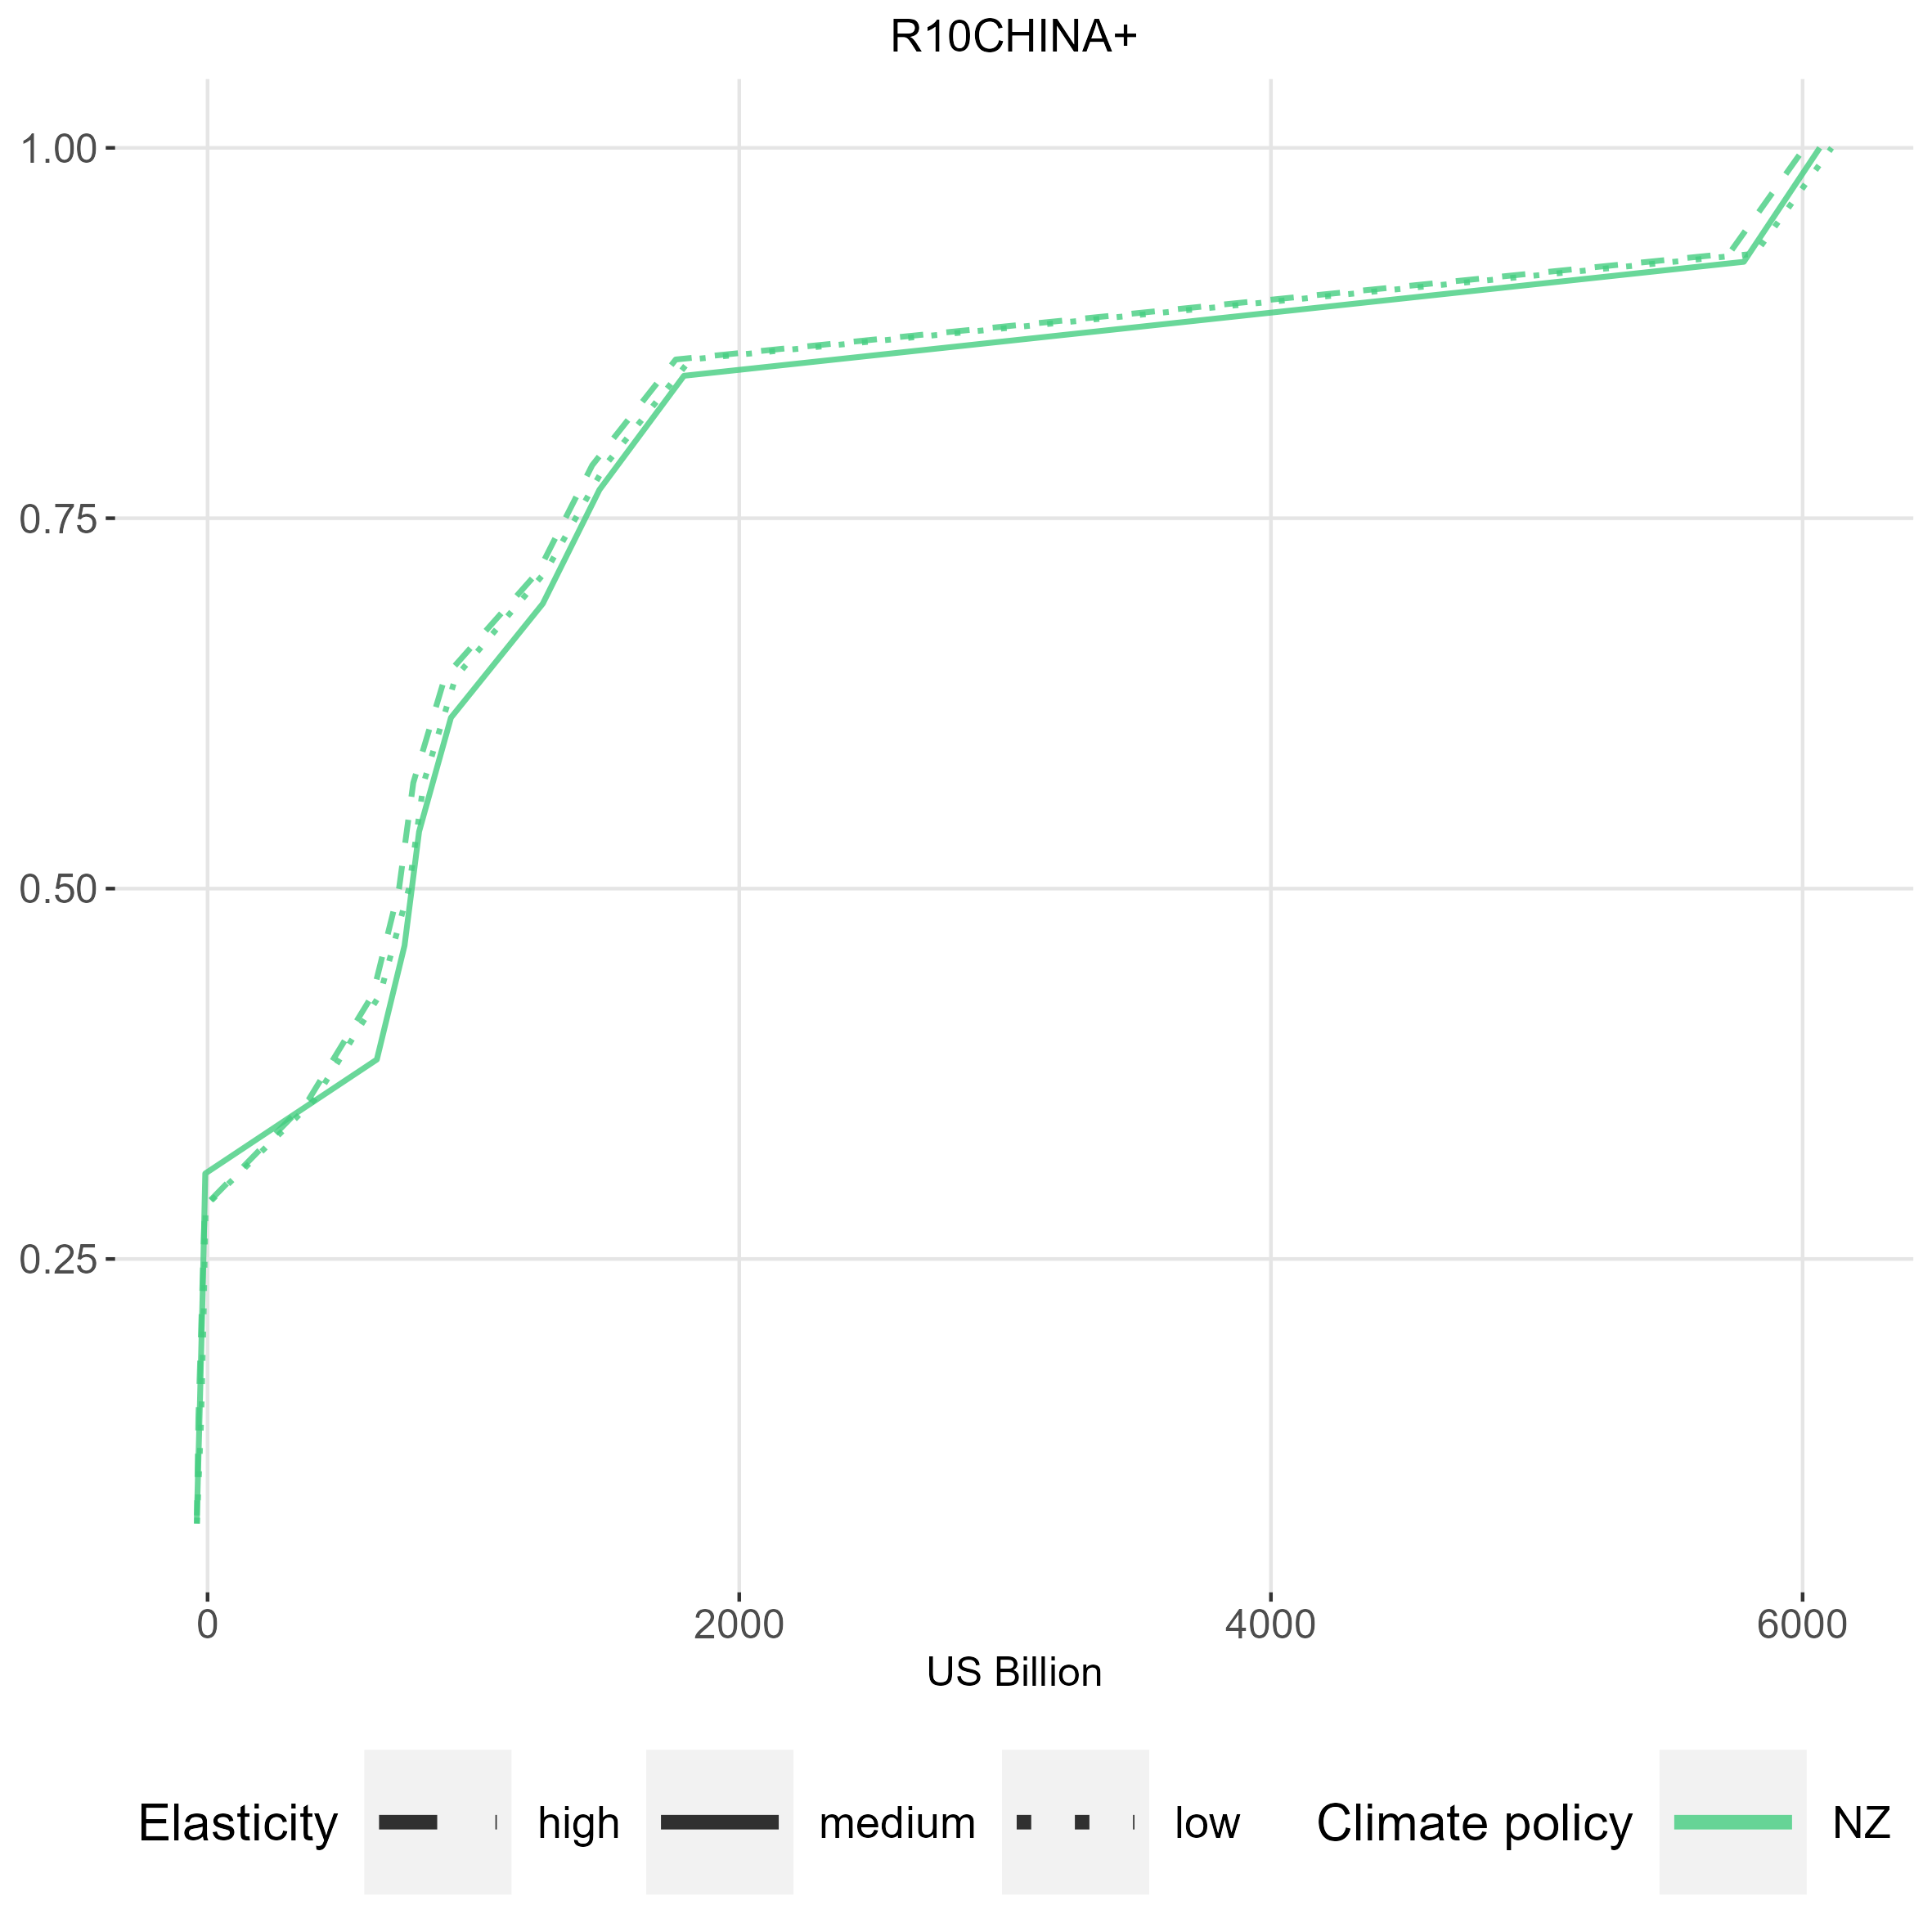
\includegraphics[width=5cm]{"Images_meth/damage_NZ/dong_NZ_median/cum_freq_dong_NZ_median_R10CHINA+.png"}};
      \node[draw=white,rectangle,rounded corners] (india_dong2) [right = of northAm_dong2] {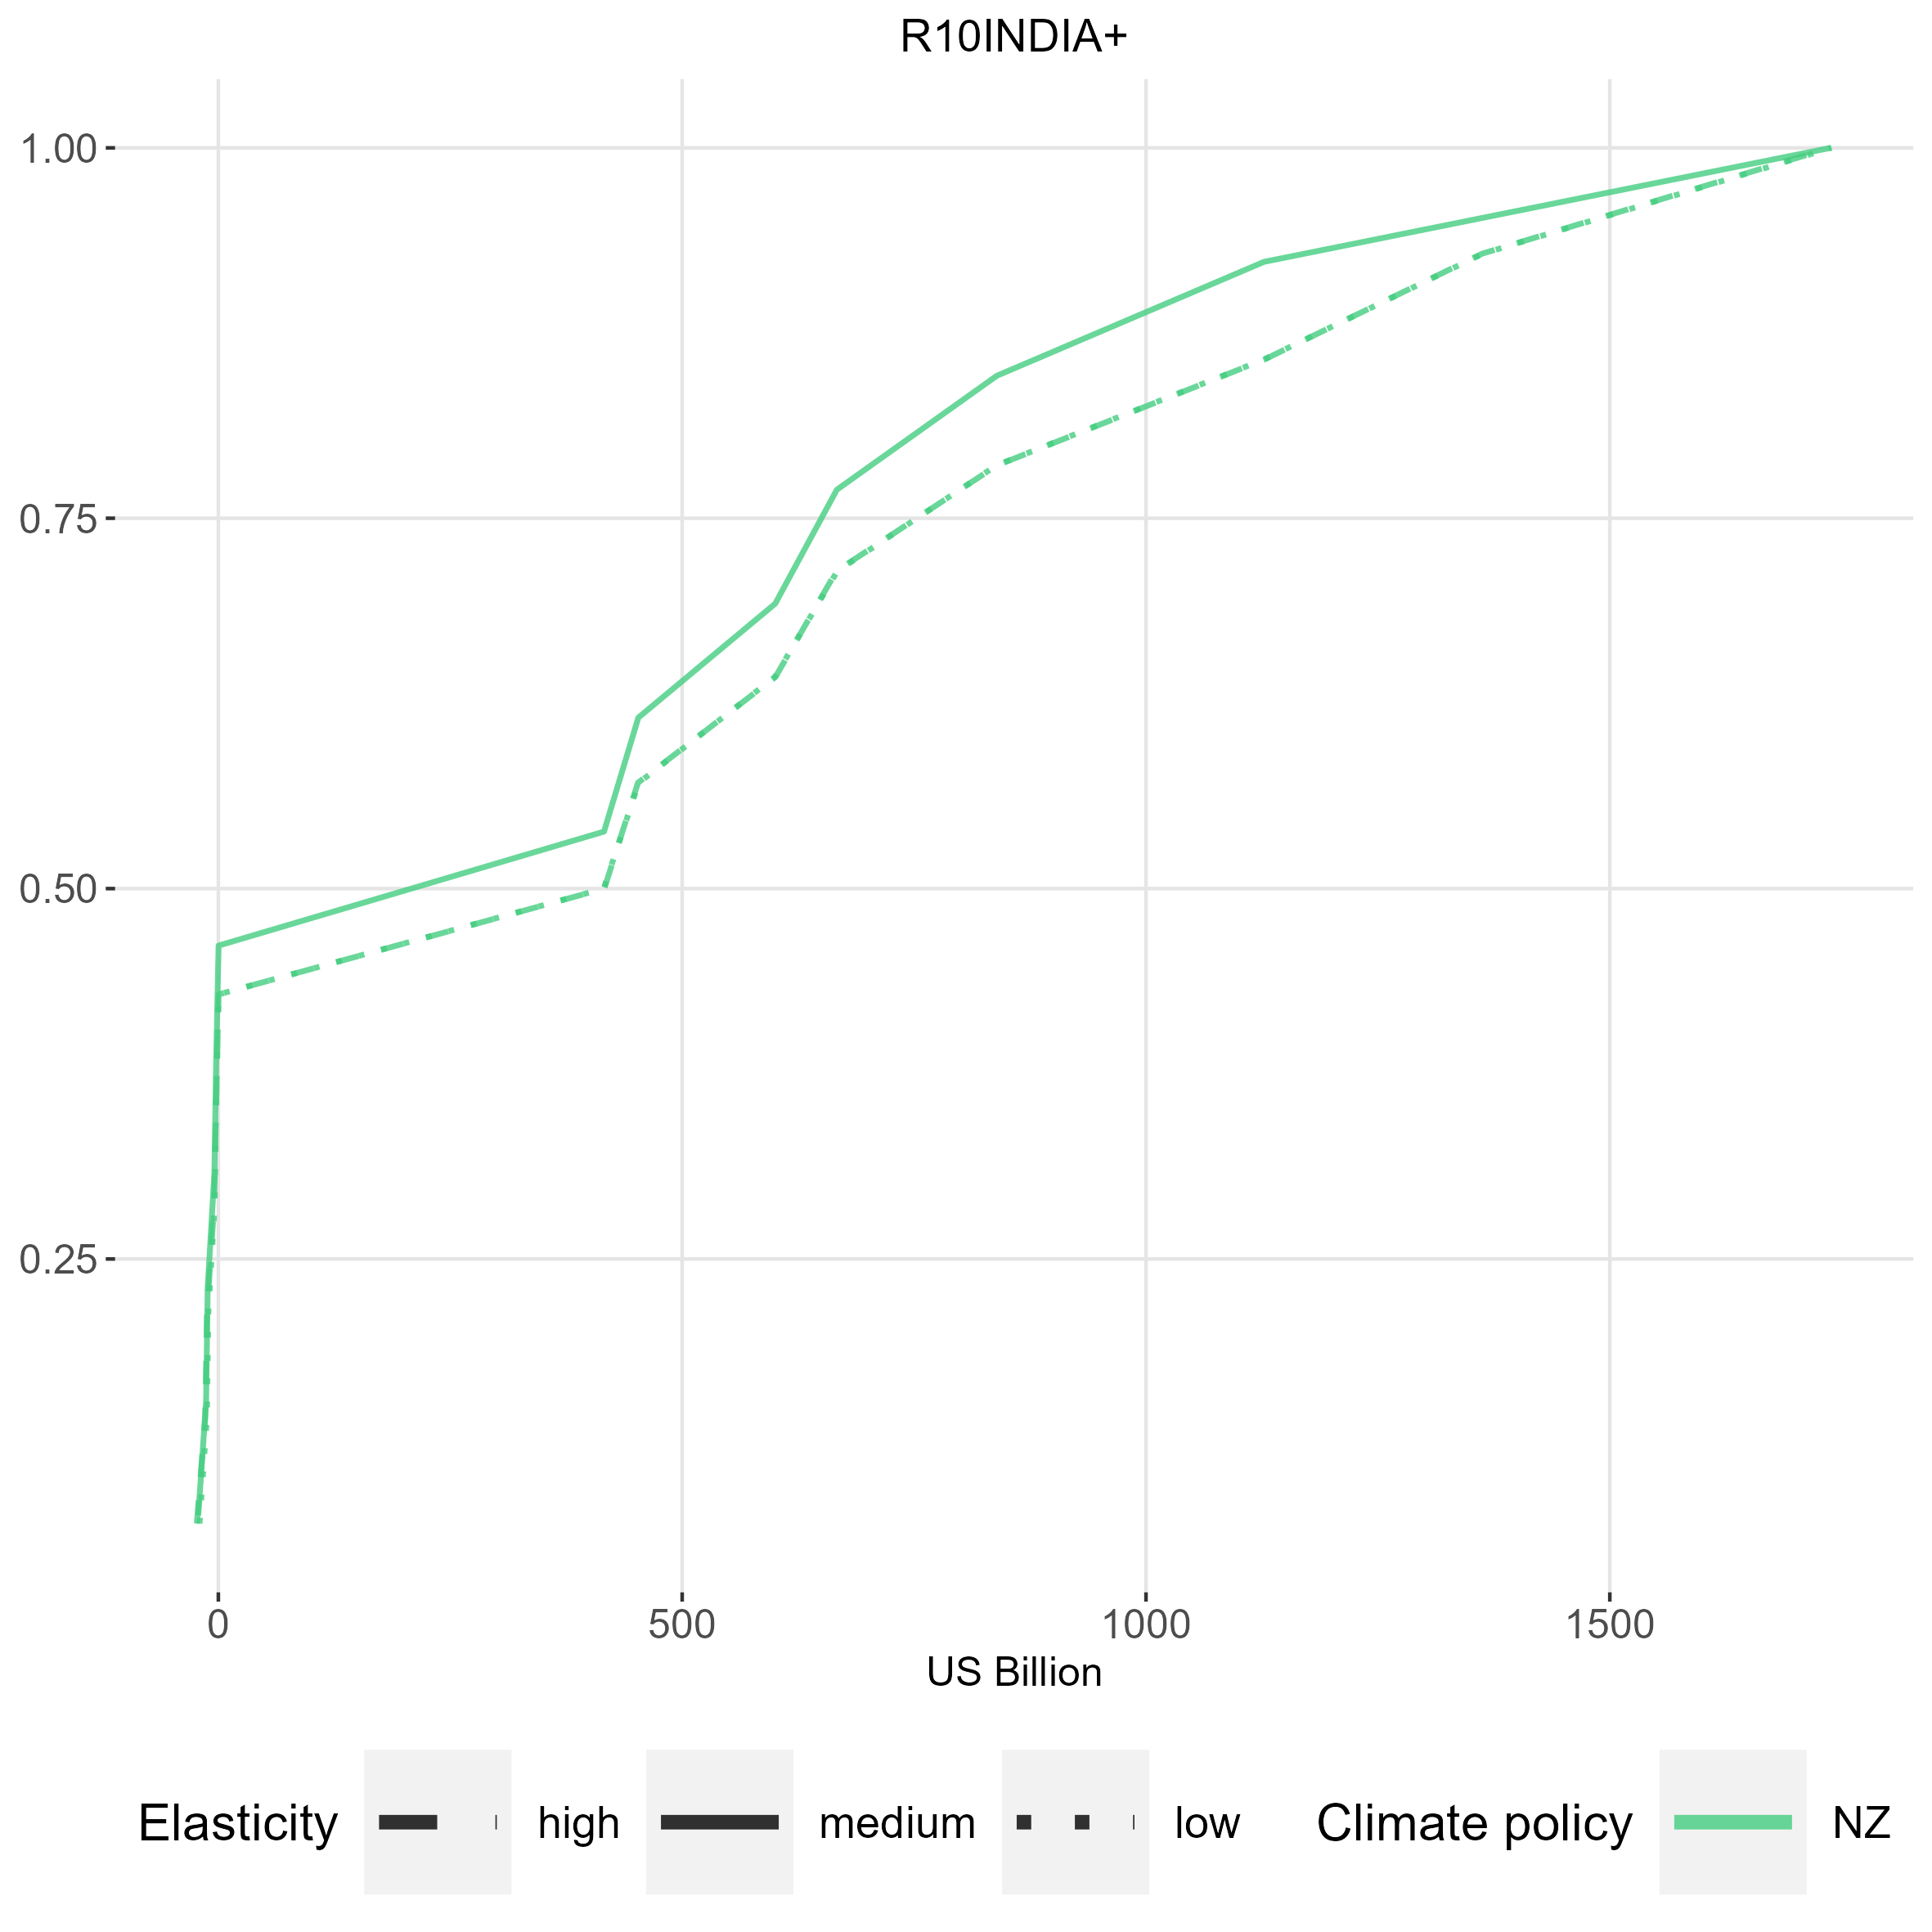
\includegraphics[width=5cm]{"Images_meth/damage_NZ/dong_NZ_median/cum_freq_dong_NZ_median_R10INDIA+.png"}};
      \node[draw=white,rectangle,rounded corners] (bb) [above = of northAm_dong2, xshift = 3cm, yshift = -0.25cm]  {\scalebox{0.7}{$AvoidedDamage_{i,t,p} = GDPnew_{i,t,p} - GDPnew_{i,t,REF}$}};
      \node[draw=white,rectangle,rounded corners] (bb) [above = of northAm_dong2, xshift = 3cm, yshift = -1cm]  {\scalebox{0.7}{$GDPgrowthNEW_{i,t} = GDPgrowthBASE_{i,t} + \beta_{i,t} AP_{i,t}, \; \beta_{i,t} = \beta_{R10CHINA, 2015} \cdot \left(\frac{GDPpc_{i,t}}{GDPpc_{R10CHINA,2015}}\right)^\alpha$}};
    \end{tikzpicture}
  \end{frame}


% Recap -----------------------------------------------------------------------
\begin{frame}
  \frametitle{Recap}
  \begin{tikzpicture}[node distance = 0.5cm]
      \node[draw=mypurple,rectangle,rounded corners, text width = 3.5cm] at (-4,0) (eng) {Detailed database};
      \node[draw=mypurple,rectangle,rounded corners, text width = 3.5cm] (emi) [below = of eng] {Estimated emissions};    
      \node[draw=mypurple,rectangle,rounded corners, text width = 3.5cm] (conc) [below = of emi] {Computed \pmm\ and \oo\ concentrations};    
      \node[draw=mypurple,rectangle,rounded corners, text width = 3.5cm] (mort) [below = of conc] {Premature deaths};    
      \node[draw=mypurple,rectangle,rounded corners, text width = 3.5cm] (econ) [below = of mort] {Economic damages};  
      
      \node[draw=mypurple,rectangle,rounded corners] at (1,-0.25) (eqDech) {\scalebox{0.75}{$\Delta ln GDP{i,t} = \gamma_{i,t} \cdot \Delta AP_{i,t}$}};
      \node[draw=mypurple,rectangle,rounded corners,anchor=west] (eqDong) at ([yshift=-1.5cm]eqDech.west) {\scalebox{0.75}{${GDPgrowthNEW{i,t} = GDPgrowthBASE_{i,t} + \beta_{i,t} \cdot AP_{i,t}}$}};
      \node[draw=mypurple,rectangle,rounded corners,anchor=west] (eqVSL) at ([yshift=-1.5cm]eqDong.west) {\scalebox{0.75}{$VSL_{i,t} = VSL_{R10EUROPE,2005} \cdot \left(\frac{GDPpc_{i,t}}{GDPpc_{R10EUROPE,2005}} \right) ^ \alpha$}};
      \node[draw=mypurple,rectangle,rounded corners,anchor=west] (eqHCL) at ([yshift=-1.5cm]eqVSL.west) {\scalebox{0.75}{$HCL_{i,t} = HC_{i,t} \cdot \Delta Mort_{i,t}$}};

      \node[above left] at ([xshift=2.8cm, yshift=-0.1cm]eqDech.north west) {$\scriptstyle{\text{\textcolor{mypurple}{Dechezleprêtre et al.}}}$};
      \node[above left] at ([xshift=1.6cm, yshift=-0.1cm]eqDong.north west) {$\scriptstyle{\text{\textcolor{mypurple}{Dong et al.}}}$};
      \node[above left] at ([xshift=0.8cm, yshift=-0.1cm]eqVSL.north west) {$\scriptstyle{\text{\textcolor{mypurple}{VSL}}}$};
      \node[above left] at ([xshift=0.8cm, yshift=-0.1cm]eqHCL.north west) {$\scriptstyle{\text{\textcolor{mypurple}{HCL}}}$};

      % Arrows
      \draw [->,mypurple] (eng) to [out=270,in=90] (emi);
      \draw [->,mypurple] (emi) to [out=270,in=90] (conc);
      \draw [->,mypurple] (conc) to [out=270,in=90] (mort);
      \draw [->,mypurple] (mort) to [out=270,in=90] (econ);
      \draw [->,mypurple] (conc) to [out=270,in=90] ++(0,-0.75) to [out=270,in=90] ++(0.5,-0.5) to [out=270,in=90] ++(0,-0.25) to [out=270,in=90] (econ);

      \only<2>{       
        \node[draw=mygray,rectangle,rounded corners, text width = 3.5cm] at (-4,0) (eng) {Detailed database};
        \node[draw=mygray,rectangle,rounded corners, text width = 3.5cm] (emi) [below = of eng] {Estimated emissions};    
        \node[draw=mygreen,rectangle,rounded corners, text width = 3.5cm] (conc) [below = of emi] {Computed \pmm\ and \oo\ concentrations};    
        \node[draw=myred,rectangle,rounded corners, text width = 3.5cm] (mort) [below = of conc] {Premature deaths};    
        \node[draw=mygray,rectangle,rounded corners, text width = 3.5cm] (econ) [below = of mort] {Economic damages};  
        
        \node[draw=mygreen,rectangle,rounded corners] at (1,-0.25) (eqDech) {\scalebox{0.75}{$\Delta ln GDP{i,t} = \gamma_{i,t} \cdot \Delta AP_{i,t}$}};
        \node[draw=mygreen,rectangle,rounded corners,anchor=west] (eqDong) at ([yshift=-1.5cm]eqDech.west) {\scalebox{0.75}{${GDPgrowthNEW{i,t} = GDPgrowthBASE_{i,t} + \beta_{i,t} \cdot AP_{i,t}}$}};
        \node[draw=myred,rectangle,rounded corners,anchor=west] (eqVSL) at ([yshift=-1.5cm]eqDong.west) {\scalebox{0.75}{$VSL_{i,t} = VSL_{R10EUROPE,2005} \cdot \left(\frac{GDPpc_{i,t}}{GDPpc_{R10EUROPE,2005}} \right) ^ \alpha$}};
        \node[draw=myred,rectangle,rounded corners,anchor=west] (eqHCL) at ([yshift=-1.5cm]eqVSL.west) {\scalebox{0.75}{$HCL_{i,t} = HC_{i,t} \cdot \Delta Mort_{i,t}$}};
  
        \node[above left] at ([xshift=2.8cm, yshift=-0.1cm]eqDech.north west) {$\scriptstyle{\text{\textcolor{mygreen}{Dechezleprêtre et al.}}}$};
        \node[above left] at ([xshift=1.6cm, yshift=-0.1cm]eqDong.north west) {$\scriptstyle{\text{\textcolor{mygreen}{Dong et al.}}}$};
        \node[above left] at ([xshift=0.8cm, yshift=-0.1cm]eqVSL.north west) {$\scriptstyle{\text{\textcolor{myred}{VSL}}}$};
        \node[above left] at ([xshift=0.8cm, yshift=-0.1cm]eqHCL.north west) {$\scriptstyle{\text{\textcolor{myred}{HCL}}}$};
  
        % Arrows
        \draw [->,mygray] (eng) to [out=270,in=90] (emi);
        \draw [->,mygray] (emi) to [out=270,in=90] (conc);
        \draw [->,mygray] (conc) to [out=270,in=90] (mort);
        \draw [->,mygray] (mort) to [out=270,in=90] (econ);
        \draw [->,mygray] (conc) to [out=270,in=90] ++(0,-0.75) to [out=270,in=90] ++(0.5,-0.5) to [out=270,in=90] ++(0,-0.25) to [out=270,in=90] (econ);
      }
  \end{tikzpicture}   
\end{frame}


